%%% The main file. It contains definitions of basic parameters and includes all other parts.

%% Settings for single-side (simplex) printing
% Margins: left 40mm, right 25mm, top and bottom 25mm
% (but beware, LaTeX adds 1in implicitly)
\documentclass[12pt,a4paper]{report}
\setlength\textwidth{145mm}
\setlength\textheight{247mm}
\setlength\oddsidemargin{15mm}
\setlength\evensidemargin{15mm}
\setlength\topmargin{0mm}
\setlength\headsep{0mm}
\setlength\headheight{0mm}
% \openright makes the following text appear on a right-hand page
\let\openright=\clearpage

%% Settings for two-sided (duplex) printing
% \documentclass[12pt,a4paper,twoside,openright]{report}
% \setlength\textwidth{145mm}
% \setlength\textheight{247mm}
% \setlength\oddsidemargin{14.2mm}
% \setlength\evensidemargin{0mm}
% \setlength\topmargin{0mm}
% \setlength\headsep{0mm}
% \setlength\headheight{0mm}
% \let\openright=\cleardoublepage

%% Generate PDF/A-2u
\usepackage[a-2u]{pdfx}

%% Character encoding: usually latin2, cp1250 or utf8:
\usepackage[utf8]{inputenc}

%% Prefer Latin Modern fonts
\usepackage{lmodern}

%% Further useful packages (included in most LaTeX distributions)
\usepackage{amsmath}        % extensions for typesetting of math
\usepackage{amsfonts}       % math fonts
\usepackage{amsthm}         % theorems, definitions, etc.
\usepackage{bbding}         % various symbols (squares, asterisks, scissors, ...)
\usepackage{bm}             % boldface symbols (\bm)
\usepackage{graphicx}       % embedding of pictures
\usepackage{fancyvrb}       % improved verbatim environment
\usepackage[square,numbers]{natbib}         % citation style AUTHOR (YEAR), or AUTHOR [NUMBER]

\usepackage[nottoc]{tocbibind} % makes sure that bibliography and the lists
			    % of figures/tables are included in the table
			    % of contents
\usepackage{dcolumn}        % improved alignment of table columns
\usepackage{booktabs}       % improved horizontal lines in tables
\usepackage{paralist}       % improved enumerate and itemize
\usepackage{xcolor}         % typesetting in color
\usepackage{float}
\usepackage{listings}
\usepackage{color}
\usepackage{multirow}
\usepackage{subcaption}
\usepackage{marginnote}
\usepackage{hyperref}
\usepackage{cleveref}

%%% Basic information on the thesis

% Thesis title in English (exactly as in the formal assignment)
\def\ThesisTitle{A Methodical Approach to the Evaluation of Appearance Computations}

% Author of the thesis
\def\ThesisAuthor{Bc. Marcel Hruška}

% Year when the thesis is submitted
\def\YearSubmitted{2020}

% Name of the department or institute, where the work was officially assigned
% (according to the Organizational Structure of MFF UK in English,
% or a full name of a department outside MFF)
\def\Department{Department of Software and Computer Science Education}

% Is it a department (katedra), or an institute (ústav)?
\def\DeptType{Department}

% Thesis supervisor: name, surname and titles
\def\Supervisor{doc. Alexander Wilkie, Dr.}

% Supervisor's department (again according to Organizational structure of MFF)
\def\SupervisorsDepartment{Department of Software and Computer Science Education}

% Study programme and specialization
\def\StudyProgramme{Computer Science}
\def\StudyBranch{Computer Graphics and Game Development}

% An optional dedication: you can thank whomever you wish (your supervisor,
% consultant, a person who lent the software, etc.)
\def\Dedication{%
I would like to express my sincere gratitude to my supervisor doc. Alexander Wilkie, Dr., for all the patience, help and advice he has given me.

I want to thank my girlfriend, my family and my friends for their constant support, especially during the last half year.
}

% Abstract (recommended length around 80-200 words; this is not a copy of your thesis assignment!)
\def\Abstract{%
Many techniques for the computation of realistic images exist, and there are a number of key technical aspects to
such systems. In addition to the light transport technique which is being used, the details of how description and
computation of object appearance are key distinguishing features. The details in questions span a wide range of
features, such as the list of BRDF and BSSDF models which are supported in a given system, to the question
whether computations are performed in colour space or in spectral form, to whether features such polarisation or
fluorescence are being supported. Although there are obvious similarities between systems, there is no standardised
implementation of any of these features, and their computation might vary in terms of accuracy.

Currently, whenever a researcher works on any aspect of appearance computation, they demonstrate their findings
on their own set of test scenes. These scenes might not necessarily cover all test scenarios, and any possible
inaccuracies might not be exposed properly.

So there is a need for an appearance test suite that would assess the correctness of such computations. The goal of
this thesis is to introduce such a set of scenes that can be used to methodically test rendering algorithms based on
their appearance reproduction capabilities. The test scenes are created in such a manner that they examine the
capabilities of the appearance computations to correctly render respective features, while neglecting other aspects
of rendering, such as global illumination. With the appearance in mind, we focus on spectral rendering in general,
as well as specialised forms of it, such as fluorescence, dispersion or polarisation. For various test cases, we
manually verify that the reference images display proper results according to the definition of respective features.
}

% 3 to 5 keywords (recommended), each enclosed in curly braces
\def\Keywords{%
{appearance},{evaluation},{spectral rendering},{iridescence},{polarization},\\{fluorescence}
}

%% The hyperref package for clickable links in PDF and also for storing
%% metadata to PDF (including the table of contents).
%% Most settings are pre-set by the pdfx package.
\hypersetup{unicode}
\hypersetup{breaklinks=true}

% Definitions of macros (see description inside)
%%% This file contains definitions of various useful macros and environments %%%
%%% Please add more macros here instead of cluttering other files with them. %%%

%%% Minor tweaks of style

% These macros employ a little dirty trick to convince LaTeX to typeset
% chapter headings sanely, without lots of empty space above them.
% Feel free to ignore.
\makeatletter
\def\@makechapterhead#1{
  {\parindent \z@ \raggedright \normalfont
   \Huge\bfseries \thechapter. #1
   \par\nobreak
   \vskip 20\p@
}}
\def\@makeschapterhead#1{
  {\parindent \z@ \raggedright \normalfont
   \Huge\bfseries #1
   \par\nobreak
   \vskip 20\p@
}}
\makeatother

% This macro defines a chapter, which is not numbered, but is included
% in the table of contents.
\def\chapwithtoc#1{
\chapter*{#1}
\addcontentsline{toc}{chapter}{#1}
}

% Draw black "slugs" whenever a line overflows, so that we can spot it easily.
\overfullrule=1mm

%%% Macros for definitions, theorems, claims, examples, ... (requires amsthm package)

\theoremstyle{plain}
\newtheorem{thm}{Theorem}
\newtheorem{lemma}[thm]{Lemma}
\newtheorem{claim}[thm]{Claim}

\theoremstyle{plain}
\newtheorem{defn}{Definition}

\theoremstyle{remark}
\newtheorem*{cor}{Corollary}
\newtheorem*{rem}{Remark}
\newtheorem*{example}{Example}

%%% An environment for proofs

\newenvironment{myproof}{
  \par\medskip\noindent
  \textit{Proof}.
}{
\newline
\rightline{$\qedsymbol$}
}

%%% An environment for typesetting of program code and input/output
%%% of programs. (Requires the fancyvrb package -- fancy verbatim.)

\DefineVerbatimEnvironment{code}{Verbatim}{fontsize=\small, frame=single}

%%% The field of all real and natural numbers
\newcommand{\R}{\mathbb{R}}
\newcommand{\N}{\mathbb{N}}

%%% Useful operators for statistics and probability
\DeclareMathOperator{\pr}{\textsf{P}}
\DeclareMathOperator{\E}{\textsf{E}\,}
\DeclareMathOperator{\var}{\textrm{var}}
\DeclareMathOperator{\sd}{\textrm{sd}}

%%% Transposition of a vector/matrix
\newcommand{\T}[1]{#1^\top}

%%% Various math goodies
\newcommand{\goto}{\rightarrow}
\newcommand{\gotop}{\stackrel{P}{\longrightarrow}}
\newcommand{\maon}[1]{o(n^{#1})}
\newcommand{\abs}[1]{\left|{#1}\right|}
\newcommand{\dint}{\int_0^\tau\!\!\int_0^\tau}
\newcommand{\isqr}[1]{\frac{1}{\sqrt{#1}}}

%%% Various table goodies
\newcommand{\pulrad}[1]{\raisebox{1.5ex}[0pt]{#1}}
\newcommand{\mc}[1]{\multicolumn{1}{c}{#1}}


% Title page and various mandatory informational pages
\begin{document}
%%% Title page of the thesis and other mandatory pages

%%% Title page of the thesis

\pagestyle{empty}
\hypersetup{pageanchor=false}
\begin{center}

\centerline{\mbox{
\includegraphics[width=166mm]{img/logo-en.pdf}}}

\vspace{-8mm}
\vfill

{\bf\Large MASTER THESIS}

\vfill

{\LARGE\ThesisAuthor}

\vspace{15mm}

{\LARGE\bfseries\ThesisTitle}

\vfill

\Department

\vfill

{
\centerline{\vbox{\halign{\hbox to 0.45\hsize{\hfil #}&\hskip 0.5em\parbox[t]{0.45\hsize}{\raggedright #}\cr
Supervisor of the master thesis:&\Supervisor \cr
\noalign{\vspace{2mm}}
Study programme:&\StudyProgramme \cr
\noalign{\vspace{2mm}}
Study branch:&\StudyBranch \cr
}}}}

\vfill

% Zde doplňte rok
Prague \YearSubmitted

\end{center}

\newpage

%%% Here should be a bound sheet included -- a signed copy of the "master
%%% thesis assignment". This assignment is NOT a part of the electronic
%%% version of the thesis. DO NOT SCAN.

%%% A page with a solemn declaration to the master thesis

\openright
\hypersetup{pageanchor=true}
\pagestyle{plain}
\pagenumbering{roman}
\vglue 0pt plus 1fill

\noindent
I declare that I carried out this master thesis independently, and only with the cited
sources, literature and other professional sources. It has not been used to obtain another
or the same degree.

\medskip\noindent
I understand that my work relates to the rights and obligations under the Act No.~121/2000 Sb.,
the Copyright Act, as amended, in particular the fact that the Charles
University has the right to conclude a license agreement on the use of this
work as a school work pursuant to Section 60 subsection 1 of the Copyright~Act.

\vspace{10mm}

\hbox{\hbox to 0.5\hsize{%
In \hbox to 6em{\dotfill} date \hbox to 6em{\dotfill}
\hss}\hbox to 0.5\hsize{\dotfill\quad}}
\smallskip
\hbox{\hbox to 0.5\hsize{}\hbox to 0.5\hsize{\hfil Author's signature\hfil}}

\vspace{20mm}
\newpage

%%% Dedication

\openright

\noindent
\Dedication

\newpage

%%% Mandatory information page of the thesis

\openright

\vbox to 0.5\vsize{
\setlength\parindent{0mm}
\setlength\parskip{5mm}

Title:
\ThesisTitle

Author:
\ThesisAuthor

\DeptType:
\Department

Supervisor:
\Supervisor, \SupervisorsDepartment

Abstract:
\Abstract

Keywords:
\Keywords

\vss}

\newpage

\openright
\pagestyle{plain}
\pagenumbering{arabic}
\setcounter{page}{1}


%%% A page with automatically generated table of contents of the master thesis

\tableofcontents

%%% Each chapter is kept in a separate file
\chapter*{Introduction}
\addcontentsline{toc}{chapter}{Introduction}

Common natural phenomena such as water reflections have always been one of the major topics discussed in the scientific circles. In the modern era of computers, many of these phenomena have already been explained and properly described by physical models. On of the ultimate interests of the computer graphics is to replicate these sensations, creating realistic images that would be indistinguishable from a photograph.

Despite the fact that the publications discussing the rendering process were released mostly in the second half of the 19th century~\cite{kajiya1986rendering}\cite{nicodemus1965directional}, it is only now that we are capable of computing certain aspects of the natural light. Mostly thanks to the more powerful hardware, correctly simulating the light transport while evaluating non-trivial physical models can be done in the matter of minutes instead of days.

As the interest in the physical realism rises also in the commercial circles such as movie industries, there is a need for more advanced light transport simulations which would bring the opportunities to create more advanced phenomena, genuine to their physical models rather than hacks and approximations.

However, as the newly-developed techniques are still being largely discussed, various rendering systems contain custom, sometimes even distinct, implementations. In addition to the light transport techniques used by the specific system, there are many other distinguishing key features, such as material models or the internal light representation. Even though large parts of the rendering systems present obvious similarities, there is no standardized implementation of any of these features, their computations vary in terms of accuracy.

These dissimilarities cause that there is no unified evaluation process that would assess the correctness of a specific technique or the whole rendering system. In fact, whenever an improved or a completely new technique is introduced, the creators present their results on their own set of scenes. Even unvoluntarily, these scenes might not properly exercise the techniques, possibly leaving some inaccuracies unexposed. Therefore, there is a need for a standardized way to test the rendering systems and their features.

\section*{Goals}

The main goal of this thesis is to introduce a set of scenes that methodically test various rendering systems based on their appearance reproduction capabilities. These scenes are specifically designed to expose potential differences between the computation of the specific phenomenon and it's defined behavior in the nature. While it is possible to test the light transport simulations, we focus on the specific appearance phenomena that are being developed and discussed to this date such as fluorescence, dispersion or polarization. Most of the evaluated phenomena absolutely need the light to be internally represented in the spectral domain so that we might simulate their looks accordingly to their physical descriptions.

For the user's convenience, we wrap the test scenes in the automated workflow and we provide the reference images that we consider to be the ground truth.

\section*{Thesis organization}

This thesis is structured as follows: 

\Cref{chap:render} introduces the reader to the color science and the computer graphics. It explains the fundamental basics of the rendering process that are a necessity to comprehend the more advanced computational models. It also defines the terminology that is widely used throughout the thesis. In case the reader is already familiar with the computer graphics field, he can skip this chapter. 

\Cref{chap:appearance} continues in discussing the specific appearance phenomena that are the main interest of this thesis, providing in-depth explanations as well as exact implementations for each of them. 

\Cref{chap:benchmark} shows the actual results of the thesis --- the evaluation suite. We describe the framework and the justifications behind its design, the test scenes that exercise the phenomena from \autoref{chap:appearance} and demonstrates the possible use case scenarios for the benchmark. 

\Cref{chap:results} directly compares the computations and their results of two different renderers.

A the end of the thesis, we provide a user guide which clarifies how to actually run and use the benchmark.


\chapter{Rendering and Color Science}
\label{chap:render}

This chapter serves as an introduction to the computer graphics and the color science. We briefly overview basic aspects of these fields, mainly to familiarize the reader with some of the fundamental processes, their backgrounds and usages. We also establish the terminology, such as \emph{rendering} or \emph{RGB color space}, that will be used throughout the thesis frequently. A significant part of the following sections is based on the publications by~\citet{wyszecki1982color},~\citet{colorScienceSlides},~\citet{nimier2019mitsuba} and~\citet{pharr2016physically}.

First, we discuss the mechanisms behind the light and colors and then we look into the process of the physically based image synthesis.

\section{Light}

According to the definition by \citet{barbrow1964international}, the light is "any radiation capable of causing a visual sensation directly". In other words, the visible light is an electromagnetic radiation that is perceivable by the human eye and allows us to see the objects around us. 

As all electromagnetic radiations, the light also propagates in form of waves. The oscillation direction of these waves does not change the color of the light but it may interact differently with the reflective/refractive objects as it passes through them. A representation of such wave propagation is displayed in \autoref{fig:wave}.

\begin{figure}[h]
	\centering
	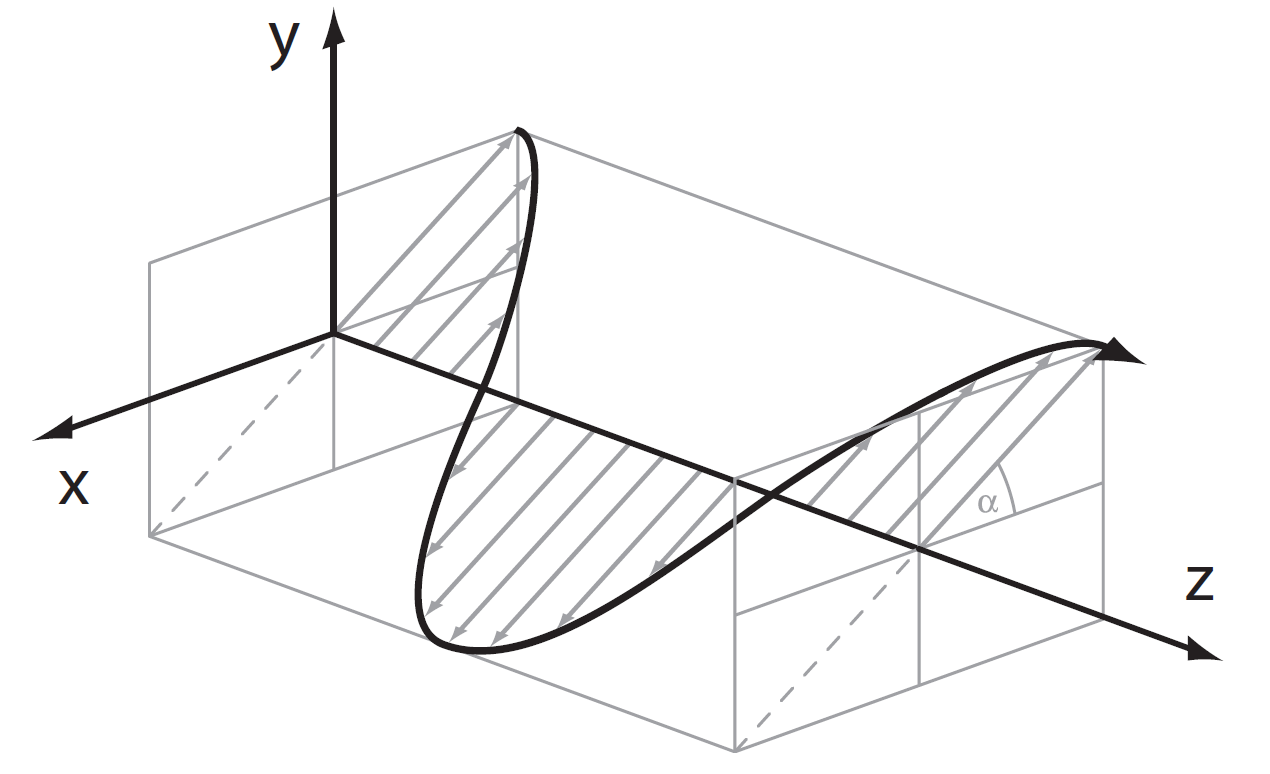
\includegraphics[width=0.7\linewidth]{img/wave.png}
	\caption{A propagation of wave~\cite{colorScienceSlides}}
	\label{fig:wave}
\end{figure}


Normally, by the term light we mean the \emph{visible light} which consists of multiple waves of unique frequencies (wavelengths). There are no exact boundaries to the visible spectrum as distinct human eyes might perceive light slightly differently but the lower boundary is estimated between 360 and 400nm and the upper boundary from 760 to 830nm~\cite{sliney2016light}. The light above this range is called infrared light and below ultraviolet. An explanatory image of the known electromagnetic wavelengths can be found in \autoref{fig:wavelengths}.

\begin{figure}[h]
	\centering
	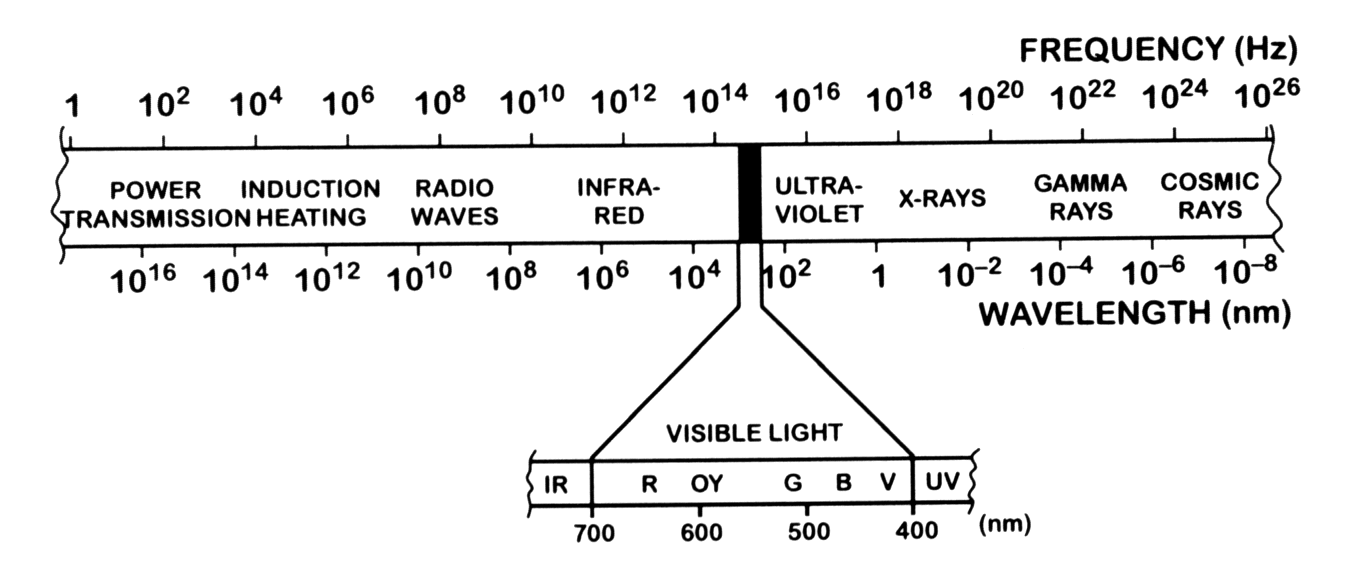
\includegraphics[width=0.8\linewidth]{img/wavelengths.png}
	\caption{An image displaying various wavelengths~\cite{colorScienceSlides}}
	\label{fig:wavelengths}
\end{figure}

\subsection{Color}

While observing an illuminated object, three different signals are sent from the eye sensors (rods and cones) to the brain, each representing a red, a green or a blue channel. When put together inside the brain, they form a sensation of the color. 

To categorize the colors, several reproducible representations were formed, called the \emph{color spaces}. A natural decision was to create an \emph{RGB color space} as it directly correlates with the signals sent from the human eyes' rods and cones. Note that multiple variations of the RGB color space exist such as \emph{sRGB} or \emph{Adobe RGB}. An illustrative comparison between several color gamuts is shown in \autoref{fig:gamut}.

\begin{figure}[h]
	\centering
	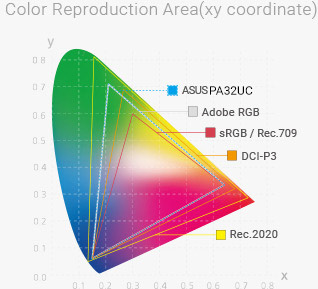
\includegraphics[width=0.6\linewidth]{img/gamut.jpg}
	\caption[ASUS RGB]{An illustrative comparison between five RGB gamuts by Asus \footnotemark}
	\label{fig:gamut}
\end{figure}
\footnotetext{\url{https://www.asus.com/Microsite/ProArtMonitor/experience-truecolor.html}}

In 1913, the Commission internationale de l'éclairage (International Commission on Illumination), shortly CIE, was formed as an authority that defines almost everything that concerns colors and their perception. In 1931, they conducted color matching experiments to obtain three color matching functions that would convert the color stimuli perceived in our eyes to the \emph{CIE RGB} color space. As these functions had a negative component, a new imaginary color space was created called \emph{CIE XYZ}. These conversions are further described in \autoref{conversion}.

CIE also defined \emph{CIE L*a*b*} color space, standard illuminants D65 and D50 and many others.

\subsection{Conversions to tristimulus color spaces}
\label{conversion}

The conversion from the spectrum to an RGB color space looks as follows:

\begin{enumerate}
	\item Compute the tristumulus value XYZ using the CIE color matching functions (shown in \autoref{fig:cmf})
	\begin{align*} 
	X=\int P(\lambda)\overline{x}(\lambda)d\lambda\\
	Y=\int P(\lambda)\overline{y}(\lambda)d\lambda\\
	Z=\int P(\lambda)\overline{z}(\lambda)d\lambda
	\end{align*} 
	, where $P(\lambda)$ is the spectral power distribution and $\overline{x}(\lambda)$, $\overline{y}(\lambda)$ and $\overline{z}(\lambda)$ are the color matching functions.
	\item Convert the XYZ to the desired RGB color space using a transformation matrix. Depending on the specific RGB color space, the matrix differs --- an example of CIE XYZ to sRGB conversion:
	\begin{align*}
	r=3.240X-0.969Y+0.55Z\\
	g=-1.537X+1.875Y-0.204Z\\
	b=-0.498+0.041Y+1.057Z
	\end{align*}
	\item (Optional) As the resulting r,g,b values may be negative, a gamut mapping might be necessary.
\end{enumerate}

\begin{figure}[httpb]
	\centering
	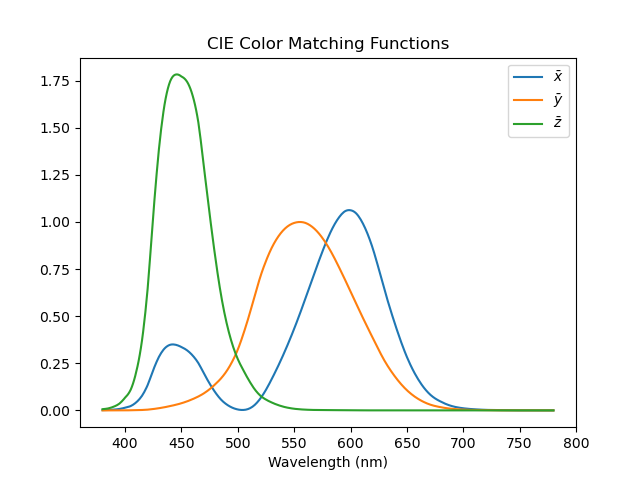
\includegraphics[width=.8\linewidth]{img/cmf.png}
	\caption[CMF]{Color matching functions plotted in Python\footnotemark}
	\label{fig:cmf}
\end{figure}
\footnotetext{The X,Y,Z data taken from \url{https://www.waveformlighting.com/tech/color-matching-function-x-y-z-values-by-wavelength-csv-excel-format}}

\subsection{Photometry and Radiometry}

Two different sets of measurement units were developed to quantify the light --- \emph{photometry} and \emph{radiometry}. The radiometry recognizes the light as an electromagnetic radiation while the photometry focuses more on the human perception of the light. Despite the distinct purposes, their quantities are often easily convertible.

\begin{tabular}{ll}
	\hline
	\textbf{Radiometric Quantity} & \textbf{Photometric Equivalent} \\
	\hline \hline
	Spectral radiant energy [$J$] & Luminous energy [$Lumen-second$] \\
	\hline
	Radiant flux [$W$] & Luminous flux [$Lumen$] \\
	\hline
	Irradiance [$W.m^{-2}$] & Illuminance [$Lumen.m^{-2}$]  \\
	\hline
	Radiant intensity [$W.sr^{-1}$] & Luminous intensity [$candela=Lumen.sr^{-1}$] \\
	\hline
	Radiance [$W.sr^{-1}.m^{-2}$] & Luminance [$candela.m^{-2}$]
\end{tabular}
\bigbreak
A brief description of each of them:
\begin{description}
	\item[Spectral radiant energy] Amount of the light energy at specific wavelength
	\item[Radiant flux] Amount of the light energy with respect to time
	\item[Irradiance] Flux at a specific point (space)
	\item[Radiant intensity] Flux in a direction (steradian, shortly $sr$, is a unit of the solid angle --- surface on a unit sphere, whole sphere has $4\pi$ steradians)
	\item[Radiance] Spatial and directional flux
\end{description}

The relationship between these quantities is described by the \emph{spectral efficiency function}. It states how efficiently a human eye reacts to different wavelengths, implying that some wavelengths are detected more easily. As we can see in \autoref{fig:lum}, the scotopic (night) perception peaks at around 507nm and the photopic (day) at 555nm.

\begin{figure}[h]
	\centering
	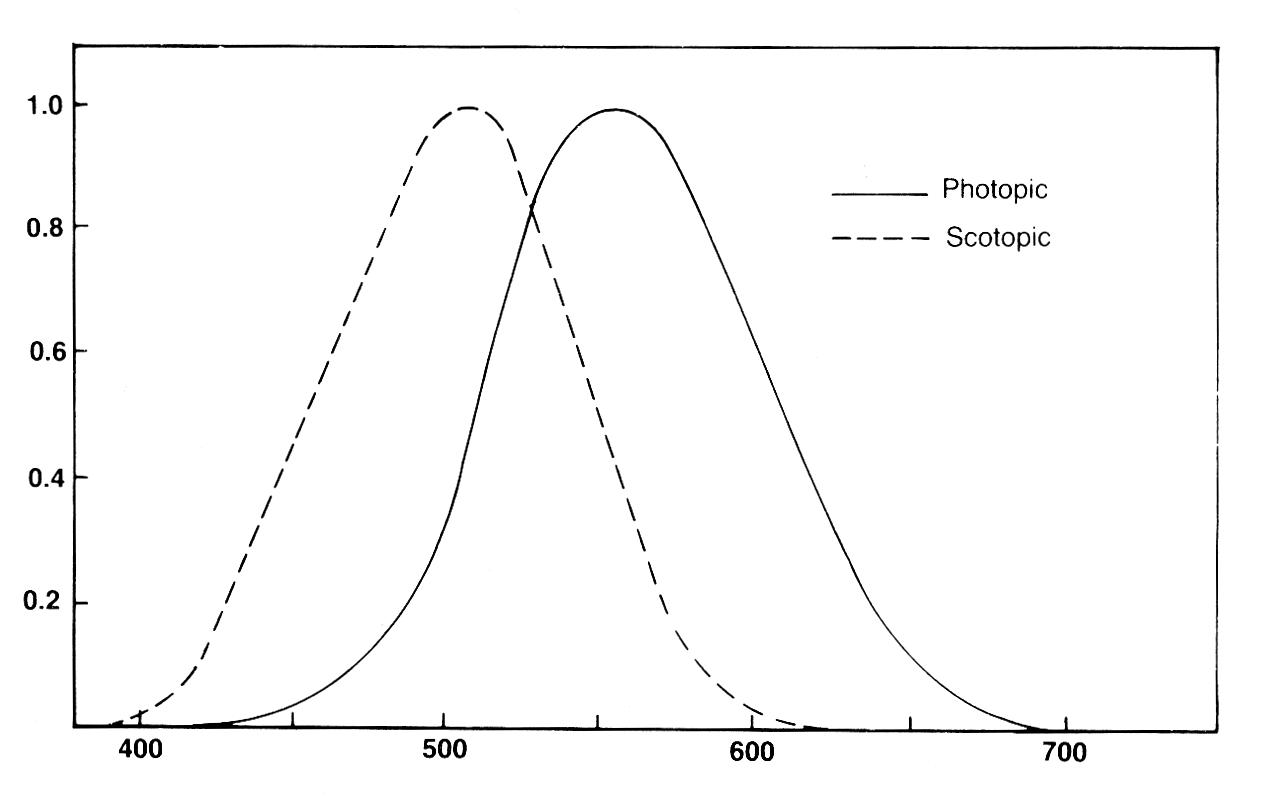
\includegraphics[width=0.8\linewidth]{img/luminous_efficiency.png}
	\caption{Relative luminous efficiency function~\cite{colorScienceSlides}}
	\label{fig:lum}
\end{figure}

\section{Physically based rendering}

One of the ultimate goals of the computer graphics is the ability to reproduce visually plausible and physically coherent images that should be indistinguishable from a photograph based on a description of a scene. Such process is called the \emph{photo realistic rendering}. In this thesis, we abbreviate the term and call it simply \emph{rendering} as the non-photo realistic one does not concern us.

The main job of a renderering system (\emph{renderer}) is to simulate various phenomena commonly seen in nature such as light reflections, refractions, shadows, etc. accurately to their physical models. These days, modern renderers are capable of recreating the scenes so authentically that the rendered images are almost identical to the real life photos. An example can be seen in \autoref{fig:corona_render}.

\begin{figure}[h]
	\centering
	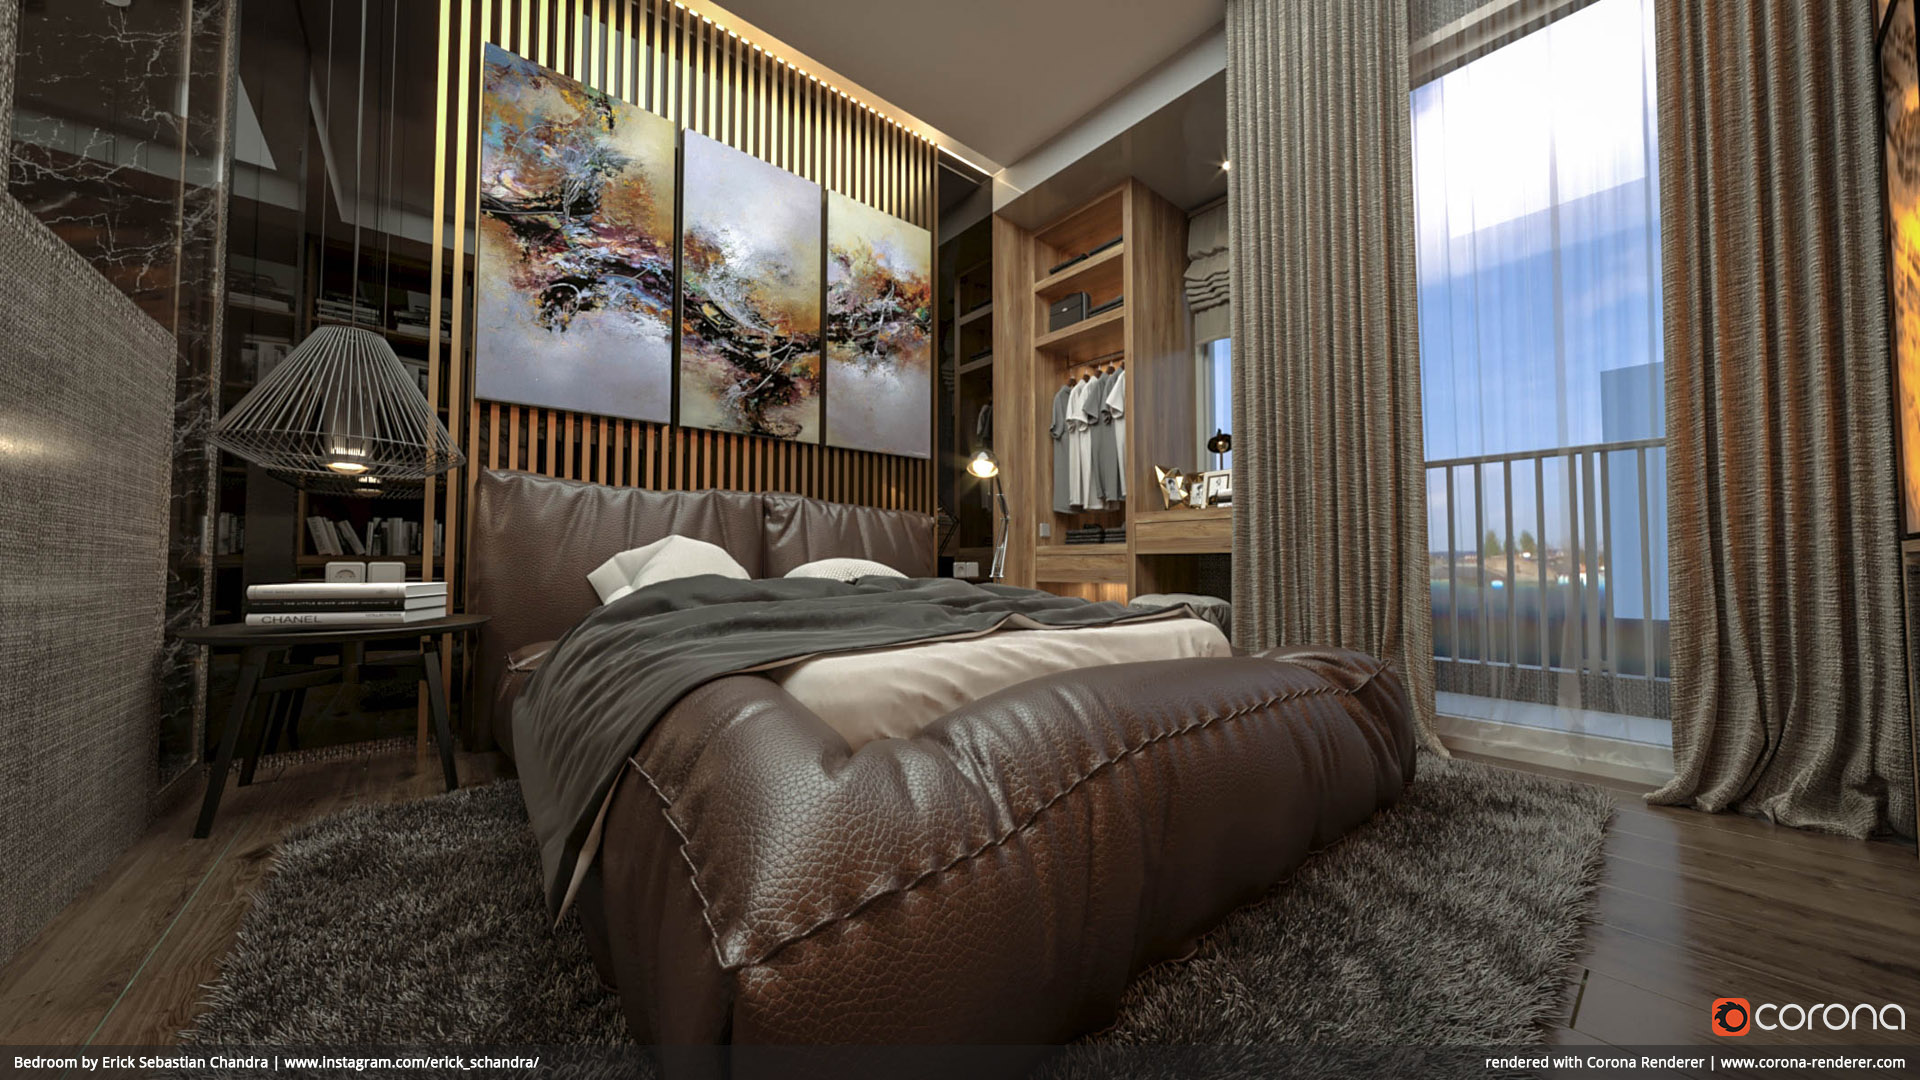
\includegraphics[width=\linewidth]{img/corona_render.jpg}
	\caption[Corona image]{An image generated with the Corona Renderer\footnotemark}
	\label{fig:corona_render}
\end{figure}
\footnotetext{\url{https://corona-renderer.com/gallery}}

The rendering workflow is similar for every renderer:
\begin{enumerate}
	\item A 3D digital scene is described by the objects it contains
	\item A light simulation algorithm runs for every visible pixel from the viewer
	\item Upon object interaction, the shading of the intersected point is computed
	\item As the algorithm terminates, a picture ("photograph") of the scene called the \emph{render} is created
\end{enumerate}

This process is further explained in \autoref{sec:light_transport}.

\subsection{Digital scene}

Basic elements of a digital scene are roughly the same for each renderer:

\begin{description}
	\item[Camera] A camera (or a sensor) in a digital scene works in the same manner as in real life --- it records a picture. Generally, you may define the coordinate position and the viewing vectors but also the properties such as focal distance or the type of the film.
	\item[Light source] The scene needs to be illuminated by one or multiple sources in order to be visible. The common kinds of lights are point light, area light, spot light or environment (constant) light. 
	\item[Objects] The actual visible contents of the scene are objects. Almost all rendering systems offer a choice to either use their prepared basic geometry such as spheres or triangles or to include a mesh geometry from an external file (usually created by a modeling software). These objects must state their material properties so that the algorithm may correctly interact with them, e.g. diffuse vs. reflective material.
\end{description}

Unfortunately, as each renderer may have a very unique implementation details, the formats of the scenes are vastly different. For example, mitsuba uses XML but PBRT has its own specific format. An example of a simple scene for Mitsuba2 can be found in \autoref{fig:example_scene}.

\definecolor{maroon}{rgb}{0.5,0,0}
\definecolor{darkgreen}{rgb}{0,0.5,0}
\lstdefinelanguage{XML}
{
	basicstyle=\ttfamily,
	morestring=[s]{"}{"},
	morecomment=[s]{?}{?},
	morecomment=[s]{!--}{--},
	commentstyle=\color{darkgreen},
	moredelim=[s][\color{black}]{>}{<},
	moredelim=[s][\color{red}]{\ }{=},
	stringstyle=\color{blue},
	identifierstyle=\color{maroon}
}

\begin{figure}[httpb]
\begin{tabular}{p{0.3\textwidth}p{0.6\textwidth}}
\begin{minipage}{0.3\textwidth}
	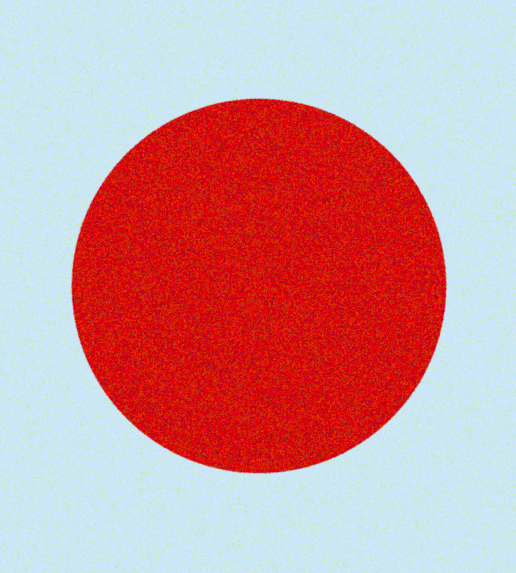
\includegraphics[width=\linewidth]{img/example_scene.png}
\end{minipage}
	&
\begin{minipage}{0.6\textwidth}
	\lstset{language=XML}
	\begin{lstlisting}[basicstyle=\tiny]
<scene version="2.0.0">
 <!-- Light transport algorithm -->
 <integrator type="path"/>
	
 <!-- Camera looking at the sphere -->
 <sensor type="perspective">
  <transform name="to_world">
   <lookat origin="0,-6,0" target="0,0,0" up="0,0,1"/>
  </transform>
 </sensor>
	
 <!-- Red sphere in the middle -->
 <shape type="sphere">
  <bsdf type="diffuse">
   <rgb name="reflectance" value="1.0,0.0,0.0"/>
  </bsdf>
 </shape>
	
 <!-- Light blue light all around the scene-->
 <emitter type="constant">
  <rgb name="radiance" value="0.6,0.8,0.9"/>
 </emitter>
</scene>
	\end{lstlisting}
\end{minipage}
\end{tabular}
\caption{A simple scene rendered with Mitsuba2 (left) along with its scene description (right)}
\label{fig:example_scene}
\end{figure}

Once the scene is described, the renderer runs a light transport simulation inside it to determine the colors of the final image. As this is a fundamental part of the rendering process, the following sections describe the physics theory and the models behind the light transport and the materials.

\subsection{BRDF}
\label{sec:BRDF}

The reflective properties of a material are described by \emph{Bidirectional Distribution Reflectance Function}, shortly \emph{BRDF}~\cite{nicodemus1965directional}. It looks as follows:

\begin{equation} \label{eq:brdf}
f_r(\omega_i,\omega_o)=\frac{dL_o(\omega_o)}{L_i(\omega_i)cos\theta_i d\omega_i}
\end{equation}

Essentialy, it states how much radiance is reflected from the incoming direction $\omega_i$ ($L_i(\omega_i)$) to the outgoing direction $\omega_o$ ($L_o(\omega_o)$) for the specific material.
An image interpretation of the function is in \autoref{fig:brdf}. As it is a distribution function, we can also reformulate its meaning as a probability density that a defined amount of light energy gets reflected from $\omega_i$ to $\omega_o$.

\begin{figure}[h]
	\centering
	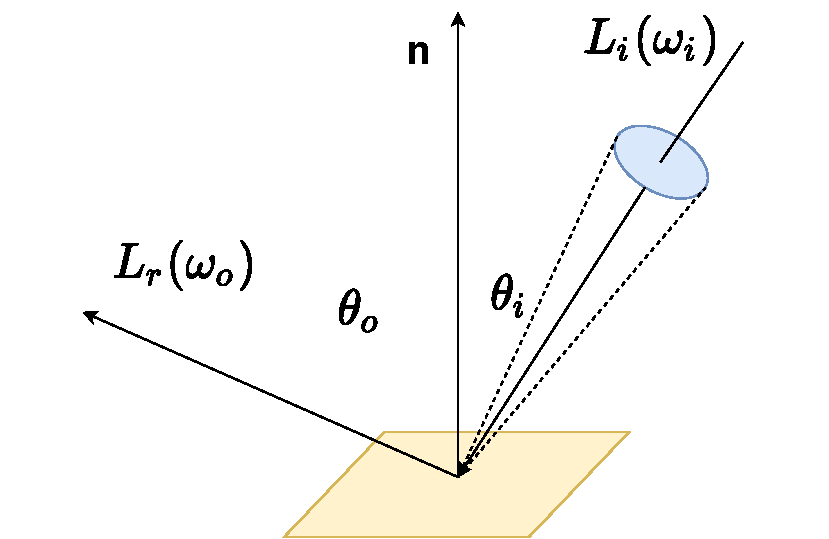
\includegraphics[width=85mm]{img/brdf.pdf}
	\caption{Bidirectional Distribution Reflectance Function}
	\label{fig:brdf}
\end{figure}

In the simplest cases, BRDF describes the reflectivity of a surface. Renders of a diffuse, a glossy and a mirror material are compared in \autoref{fig:compare_brdf}.

\begin{figure}[httpb]
	\begin{tabular}{ccc}
		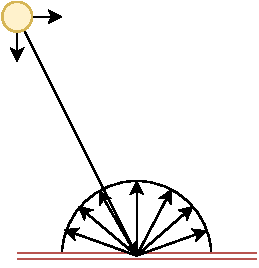
\includegraphics[width=.3\linewidth]{img/brdf_diffuse_diag.pdf}
		&
		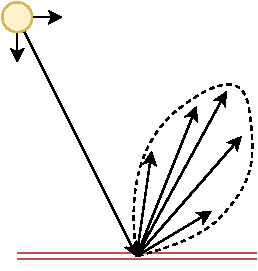
\includegraphics[width=.3\linewidth]{img/brdf_glossy_diag.pdf}
		&
		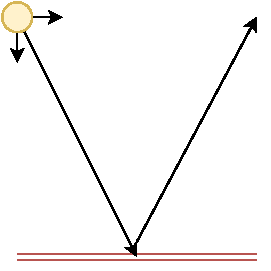
\includegraphics[width=.3\linewidth]{img/brdf_mirror_diag.pdf} \\
		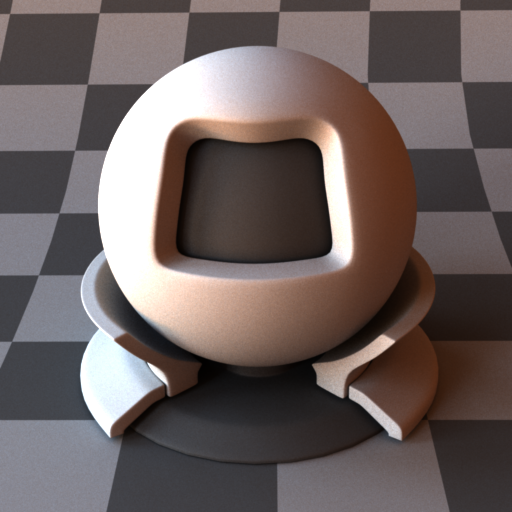
\includegraphics[width=.3\linewidth]{img/brdf_diffuse.png}
		&
		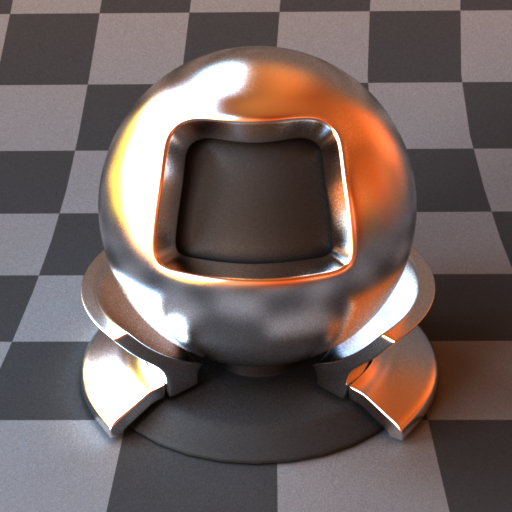
\includegraphics[width=.3\linewidth]{img/brdf_glossy.png}
		&
		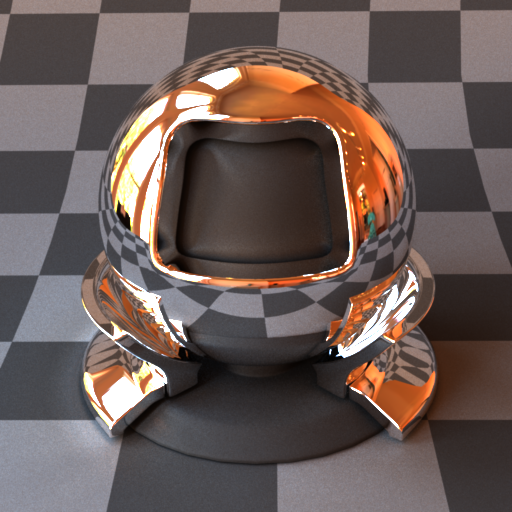
\includegraphics[width=.3\linewidth]{img/brdf_mirror.png}
	\end{tabular}
	\caption{A preview of a diffuse (left), a glossy (middle) and mirror (right) material rendered in Mitsuba2 along with their illustrative BRDF visualizations}
	\label{fig:compare_brdf}
\end{figure}


Physically based BRDFs must fulfill several properties~\citealp{duvenhage2013numerical}:
\begin{description}
	\item[Heimholtz reciprocity] The amount of reflected energy from the incoming direction to the outgoing direction is equal to the amount of energy in the reversed directions ($f_r(\omega_i,\omega_o)=f_r(\omega_o,\omega_i)$).
	\item[Energy conservation] The amount of reflected energy cannot be larger than all received energy.
	\item[Positivity] BRDF is always positive ($f_r(\omega_i,\omega_o)\ge0$).
\end{description}

Note that BRDF concerns only opaque surfaces. There exist multiple distribution functions that describe behavior of other materials, for example:
\begin{description}
	\item[BTDF] Describes light transmission
	\item[BSDF] Combination of BTDF and BRDF (e.g. glass, water)
	\item[BSSRDF] Considers scattering of the light under the surface as well (e.g. skin)
\end{description}

In this thesis, most of the materials that we talk about are actually described by BSDF.

\subsection{Global Illumination}

With the BRDF defined, we can now formulate an equation that evaluates the global illumination of a scene --- illumination of each point from all light sources. It is generally called the \emph{rendering equation}~\cite{kajiya1986rendering}:

\begin{equation}
L_o(x,\omega_o)=L_e(x,\omega_o)+L_r(x,\omega_o)
\end{equation}

Let's break it down first:
\begin{description}
	\item[$x$] is the currently computed point in the scene.
	\item[$L_o$] is the outgoing radiance.
	\item[$L_e$] is the radiance emitted by $x$ as $x$ can be on a light source.
	\item[$L_r$] is also called the \emph{reflectance equation} and it states the total amount of the reflected radiance for all contributions of the incident radiance. Hence, it is an integral over the upper hemisphere over $x$ that look as follows:
	\begin{equation}
	L_r(x,\omega_0)=\int_{\Omega}f_r(x,\omega_o,\omega_i) L_i(x,\omega_,i) cos\theta_i d\omega_i
	\end{equation}
	, where
	\begin{description}
		\item[$f_r(x,\omega_o,\omega_i)$] is the BRDF of $x$ as defined in \autoref{eq:brdf}.
		\item[$L_i(x,\omega_i)$] is the incoming radiance from a light source.
	\end{description}
\end{description}

An image interpretation of the reflectance equation can be seen in \autoref{fig:refl}.

\begin{figure}[h]
	\centering
	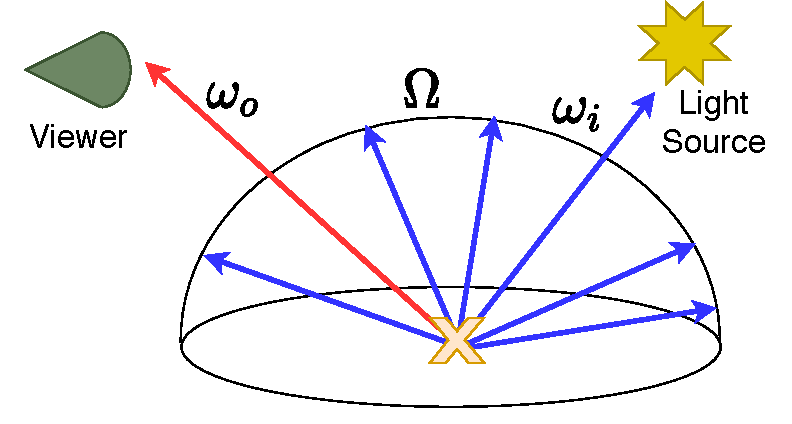
\includegraphics[width=85mm]{img/refl.pdf}
	\caption{Reflectance Equation}
	\label{fig:refl}
\end{figure}

As a matter of fact, each light transport algorithm tries to solve some of the formulations of the rendering equation.

Interestingly, the light transport is recursive in nature. As we can see from the rendering equation, to compute the outgoing radiance at a certain point $x$, we need to know all the contributed incoming radiances. These do not necessarily have to originate at a light source --- the incoming radiance may come from another, non-emitting point $y$ in the scene as a result of the rendering equation computed at the point $y$.

\subsection{Monte Carlo integration}
Before we proceed to the actual algorithms that evaluate the rendering equation, we briefly introduce a method that is used to approximate the definite integral --- \emph{Monte Carlo integration}~\cite{caflisch1998monte}.

Formally, for a multidimensional definite integral
\begin{equation}
I=\int_{\Omega}g(x)dx
\end{equation}
 Monte Carlo (MC) estimates I as 
 \begin{equation}
 \langle I\rangle=\frac{1}{N}\sum_{k=1}^{N}\frac{g(\xi_k)}{p(\xi_k)}; \xi_k\propto p(x)
 \end{equation}

\begin{figure}[H]
	\centering
	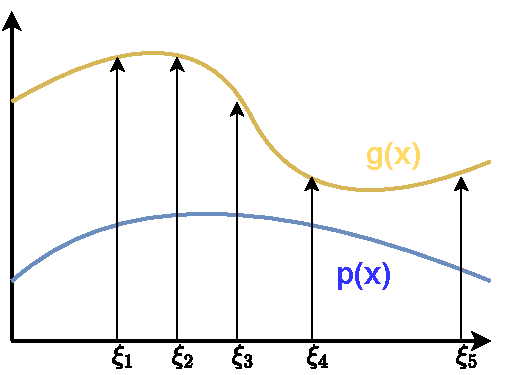
\includegraphics[width=0.5\linewidth]{img/monte_carlo.pdf}
	\caption{Monte Carlo method 2D visualization}
\end{figure}

In other words, Monte Carlo is a non-deterministic method that sums N randomly chosen samples $\xi_k$, computes their values $g(\xi_k)$ and averages them. To reduce variance, an importance sampling is introduced by drawing samples from a distribution $p(x)$ that is chosen for each specific problem to approximate the former $g(x)$ function. In reality, the importance sampling ensures that if some samples are generated twice as much, their weight is decreased to half.

There exist other methods that are used to approximate integrals such as deterministic quadrature or Markov Chain Monte Carlo (MCMC).

\subsection{Light transport algorithms}
\label{sec:light_transport}

\subsubsection{Path tracing}
Over the years, a large number of various light transport algorithms and their variations have been developed, where each has its own benefits. The one that we mention the most in this thesis is called the \emph{path tracing}. Its core idea is simple:

\renewcommand{\labelenumii}{\theenumii}
\renewcommand{\theenumii}{\theenumi.\arabic{enumii}.}
\begin{enumerate}
	\item For each pixel in the image plane, shoot a primary ray $r$ from camera into the scene.
	\item If $r$ hits a non-emitting object at point $x$:
	\begin{enumerate}
		\item Compute BRDF at $x$.
		\item Generate a new random direction $\omega$. Ideally, the distribution of the generated direction should be proportional to the BRDF --- e.g. diffuse BRDF would generate a direction  uniformly over a hemisphere while glossy BRDF would prioritize samples from the reflectance lobe (look at \autoref{fig:compare_brdf}).
		\item Add the BRDF value to the final color of the pixel.
		\item Check for a terminating condition --- there exist several options, usually a combination of them is applied:
			\begin{description}
				\item [Maximum depth] User specified maximum number of recursions.
				\item [Russian Roulette] Randomly choose if the ray survives, lowering the chance with each consecutive bounce.
				\item [BRDF-proportional] Depending on the surface material, decide whether the ray survives or not. For example, reflective or refractive surfaces need a lot more recursions as they propagate the light further to the scene than diffuse surfaces.
			\end{description}
		\item In case the termination was not successful, bounce -- shoot a secondary ray $r$ from the point $x$ in the direction $\omega$ and continue from step 2.
	\end{enumerate}
	\item If $r$ hits an emitting object (light source), add its emission $L_e$ to the final color of the pixel
	\item If no scene geometry is hit, terminate the algorithm and add the color of the surrounding light (if there is any).
\end{enumerate}

The bouncing of the light in the scene nicely correlates with the recursive nature of the rendering equation. Even though the path tracing is a slow algorithm (i.e. not suitable for real-time rendering in games), its variations can be extremely accurate. Providing equally accurate surface models used in the scene, the resulting images might even be indistinguishable from real photographs. 


\paragraph{MIS}

In the algorithm described above, the direct illumination computation of each scene intersection is dependent only on the BRDF of the intersected surface and consequent walk to the light source. However, such scenario that the light source is hit at the end of every walk is greatly dependent on the number of samples and the maximum allowed depth of the recursion. Consequently, this creates variance which can be easily improved the integration of the \emph{multiple importance sampling} (MIS). Generally, it involves a weighted combination of multiple sampling techniques. Typically, it combines the BRDF proportional sampling and the light source sampling --- in each step of the path tracing, every light source that is visible from the intersected point contributes to its value. Both sampling methods are, of course, weighted to avoid an over-illumination. 

\paragraph{Volumes}

Another aspect that needs to be accounted for in the rendering process are volumetric objects such as fogs or smokes. Normally, there are two ways that a volumetric object may effect the light passing through it. The volume is either attenuating the light by absorbing it or scattering to different directions. Or the volume can also strengthen it by emitting light (e.g. flame) or scattering light from different directions to the sampled one.

A single walk of a path tracer capable of volume tracing and MIS sampling is visualized in \autoref{fig:path_tracer_vis}.

\renewcommand\thesubfigure{\arabic{subfigure}}
\begin{figure}
	\begin{tabular}{cc}
		\begin{subfigure}
			{0.45\textwidth}\centering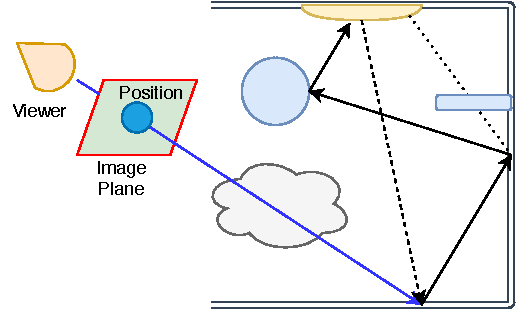
\includegraphics[width=\linewidth]{img/path_tracer_step1.pdf}
			\caption{Primary ray created}
		\end{subfigure}
		&
		\begin{subfigure}
			{0.45\textwidth}\centering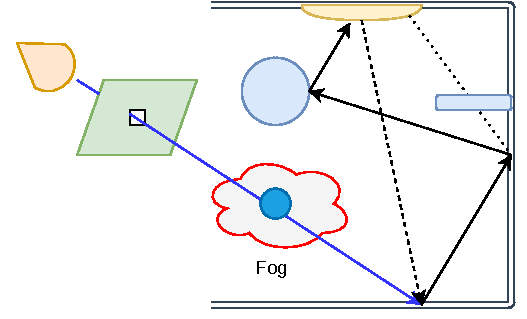
\includegraphics[width=\linewidth]{img/path_tracer_step2.pdf}
			\caption{Passing volume, attenuation}
		\end{subfigure} \\
		\begin{subfigure}
			{0.45\textwidth}\centering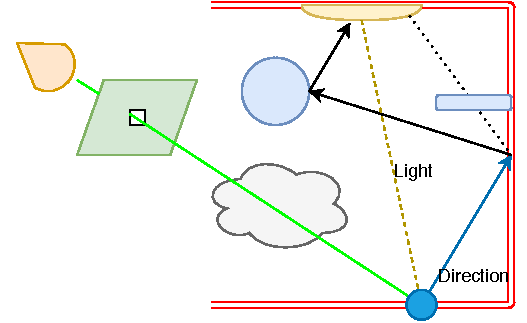
\includegraphics[width=\linewidth]{img/path_tracer_step3.pdf}
			\caption{ Geometry hit, new direction, BRDF + light added}
		\end{subfigure} 
		&
		\begin{subfigure}
			{0.45\textwidth}\centering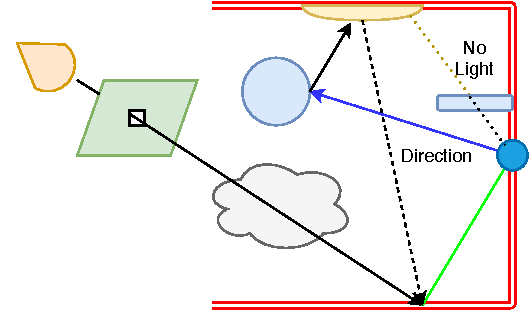
\includegraphics[width=\linewidth]{img/path_tracer_step4.pdf}
			\caption{Geometry hit, new direction, BRDF added (light obscured)}
		\end{subfigure} \\
		\multicolumn{2}{c}{		
		\begin{subfigure}
				{0.45\textwidth}\centering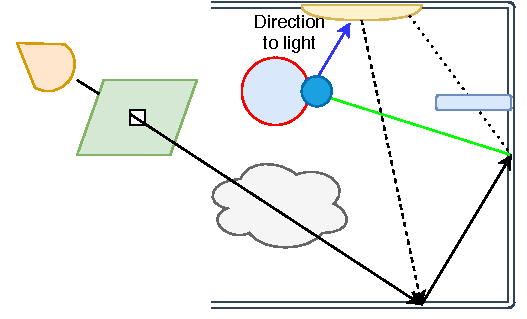
\includegraphics[width=\linewidth]{img/path_tracer_step5.pdf}
				\caption{Geometry hit, new direction points to light, add contribution and terminate}
		\end{subfigure}}
	\end{tabular}
	\caption{A visualization of a single walk in path tracer}
	\label{fig:path_tracer_vis}
\end{figure}


\subsubsection{Other methods}
As the path tracing is of our main concern in this thesis due to its physically based and unbiased properties, some of the other global illumination techniques are described only briefly here:

\begin{description}
	\item[Ray tracing]\cite{glassner1989introduction} Similar to the path tracing but there are no bounces from the surfaces, simulates only reflections, refractions, scattering etc. These days, real-time rendering is capable of ray tracing.
	\item[Photon mapping]\cite{jensen2001realistic} Two rays are traced independently --- from the camera and from the light source until termination occurs, then the radiance is computed based on their final positions. Faster at some scenarios but biased (does not have to converge to a correct solution).
	\item[Radiosity]\cite{sillion1994radiosity}Uses the finite element method instead of Monte Carlo. View independent, the light is traced from the source and bounced (possibly) to the viewer. Good for precomputations. 
\end{description}

\section{Spectral Rendering}

So far, we've considered the colors to be internally represented by a tristimulus color space during the rendering process. For the explanation purposes, let's assume RGB color space --- colors of all objects in the scene are defined in RGB, the path tracing step colors are RGB and the output color is RGB. In a large number of scenarios, this workflow is sufficient as we are capable of simulating a majority of the common aspects (e.g. optics) while keeping the rendering simple and robust. Unfortunately, the RGB color space is only a fraction of the visible gamut and has no notion of the light as an electromagnetic radiation. Consequently, we are loosing a significant amount of information, causing the colors to be at times inaccurate and some phenomena completely impossible to render. 

Therefore, a new approach to the rendering has been introduced that internally represents the colors as a spectrum distribution function instead of a tristimulus color space --- the \emph{spectral rendering}. The core idea is to track and sample several wavelengths at once for each step of the path tracing and to perform the integration over all of them. We also generalize the BSDF to account for the wavelengths: $f_r(\lambda,\omega_i,\omega_o)$.

Most of the phenomena evaluated in this thesis are a direct consequence of the light's nature as an electromagnetic radiation, hence the primary focus is placed on the spectral rendering.
The following sections are largely based on a publication by \citet{wilkie2002tone}.

\subsection{Color representation}

If the spectral rendering is desired, some representation of the spectral distribution functions needs to be implemented. While several techniques are feasible, it is often a matter of a simple trade-off between the precision and the performance. For example, sampling wavelengths uniformly each 5nm would yield significantly more accurate results than sampling only four wavelengths in total. However, such approach might become unbearable in terms of speed and memory. Moreover, the spectral functions are usually quite smooth, therefore such dense sampling is mostly completely unnecessary. Some examples of these functions can be seen in \autoref{fig:spectral_color}.

A typical approach is to sample at larger ranges (more than 10 nanometers) and use basis functions for the representation~\cite{peercy1993linear}. More approaches and their details are briefly explained by \citet{wilkie2002tone}.

\begin{figure}[httpb]
	\centering
	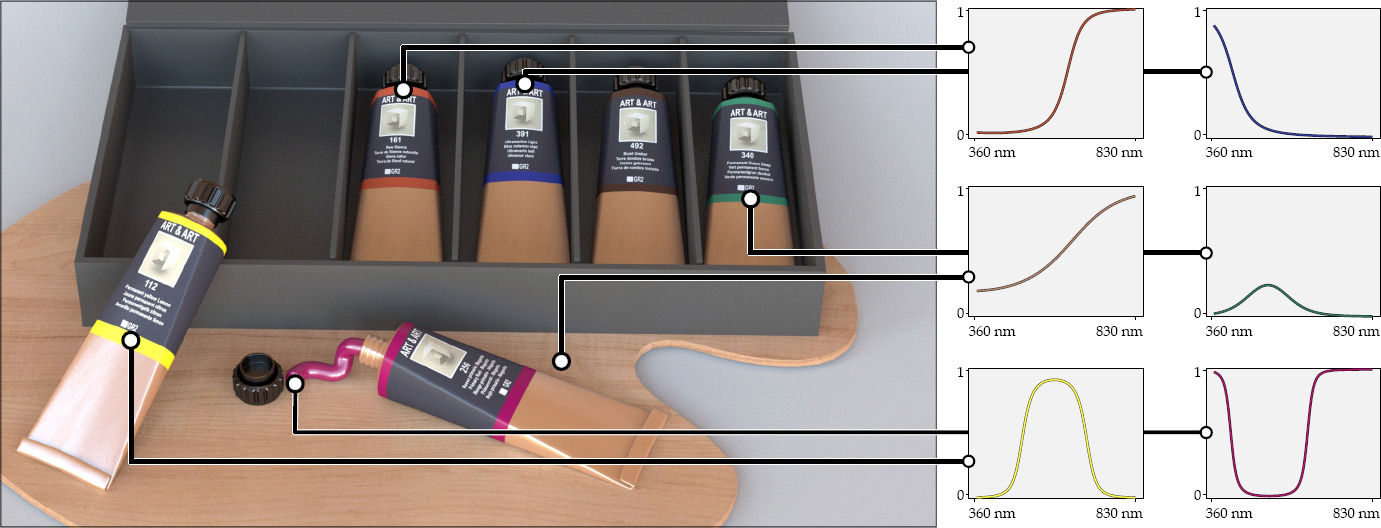
\includegraphics[width=.9\linewidth]{img/spectral_color.jpg}
	\caption{Spectral curves measured for different colors\cite{jakob2019low}.}
	\label{fig:spectral_color}
\end{figure}

\subsection{Advantages}

The spectral rendering presents the ability to reproduce the colors in a more photorealistic way. We might not see it at first, but the colors produced by a conventional RGB renderer tend to be slightly over-saturated as they do not account for the spectral characteristics of the light which might attenuate the final color. A comparison between the RGB and the spectral render of the same scene by Mitsuba2 is shown in \autoref{fig:compare_color}.

\begin{figure}[httpb]
	\begin{tabular}{cc}
		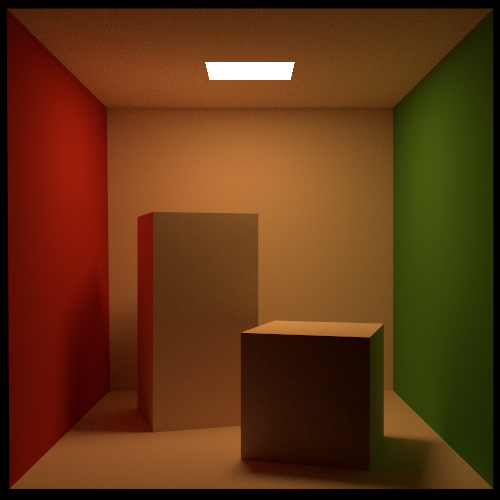
\includegraphics[width=.45\linewidth]{img/rgb.jpg}
		&
		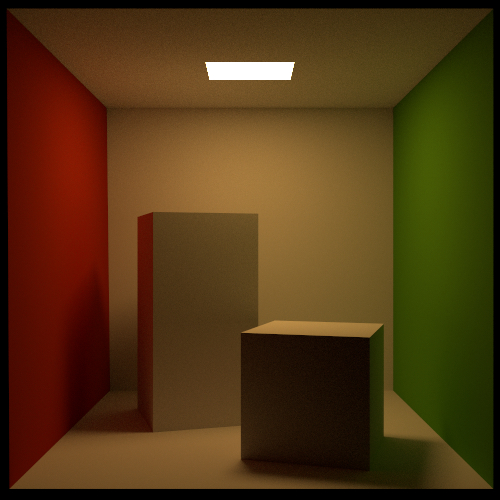
\includegraphics[width=.45\linewidth]{img/spectral.jpg}
	\end{tabular}
	\caption{A comparison between the RGB render (left) and the Spectral render (right) of the same scene by Mitsuba2~\cite{mitsubaWeb}}
	\label{fig:compare_color}
\end{figure}

Still, the biggest advantage is the possibility to reproduce some of the natural phenomena for which the tracing of multiple wavelengths is an absolute necessity. Namely, those are:
\begin{description}
	\item[Fluorescence] Absorption and re-emission of a different color
	\item[Dispersion] Splitting of the white light into its wavelength components via refraction
	\item[Polarisation] Change of the oscillation direction of a light wave 
	\item[Iridescence] Thin layer constructive/destructive light interference
\end{description}
They are explained in detail in \autoref{chap:appearance}.

\subsection{Disadvantages}

On the other side, the need to numerically integrate over multiple wavelengths introduces a problem of the chromatic noise. Fortunately, this has been effectively eliminated by the introduction of \emph{Hero Wavelength Spectral sampling}~\cite{wilkie2014hero}. Also, even though the performance is not a key factor, it obviously worsens as well. 

Moreover, it is quite possible that the spectral images won't ever be properly displayable on the screens. Even the most modern monitors use a color space that is still smaller than the gamut of human-perceived colors. The only viable way is to store the distinct spectral bands as separate images. Clearly, it is quite inconvenient to have multiple results instead of one as it does not correlate with the images that we capture in reality. Therefore, the rendering needs to have a well-done spectrum to final RGB conversion as the final image is still being displayed on an RGB monitor. Fortunately, the conversion is well-defined and fairly simple to implement.

Due to the fact that the RGB gamut is only a subset of the visible spectrum, the situation gets significantly more complicated for the reversed conversion. As there exist infinitely many spectra for one RGB value, several techniques were proposed to convert the tristimulus to the spectral domain --- commonly called the \emph{spectral upsampling}. For those who may be interested in the details of the current development to the spectral upsampling, refer to the article by \citet{jakob2019low} which proposes a solution that is capable of converting full sRGB gamut with zero error.

Obviously, it is also possible to simply map RGB values to their measured data. However, this requires a lot of manual work as the same "color" (reflective spectrum) might have to be measured for various lighting conditions and mapped accordingly.

There exist several reasons to integrate the spectral upsampling, mainly because the spectral values are a lot harder to obtain and to use. You need a specific device (spectrometer) that would measure the color values under a specific light and then use regularly distributed samples from it as an input. Because of the reproducibility of the RGB color space and its legacy usage (lots of existing textures are already defined in RGB), it is a lot more convenient to input the values of textures as RGB values, convert them internally to the spectral domain and convert them back to the desired color space for the output image.

\chapter{Appearance Computations}
\label{chap:appearance}

So far, we've covered the fundamental basics of the light and the rendering process to be able to comprehend the more advanced techniques practiced in the computer graphics. As we've mentioned before, our primary goal is to evaluate the computational accuracy of several specific appearance sensations. Even though they are quite common in every day life, their integration to the modern renderers is, to this date, rare.  In this chapter, we discuss these phenomena individually --- their manifestations in the nature, the physics behind them and finally, their computations in the rendering process. 

\section{Reflectance}

The reflective surfaces are a surprisingly common sighting. As the perfectly diffuse materials basically do not exist in the nature, a large set of the materials that surround us are considered glossy. In \autoref{sec:BRDF}, we explained the bidirectional reflectance distribution function that defines the reflective properties of a material. 

\subsection{Fresnel equations}

It is necessary to know the basics of the geometry optics to be able to properly define a reflectance model. First of all, the \emph{Snell's law}~\cite{pharr2016physically}

\begin{equation}
\eta_i sin\theta_i = \eta_t sin\theta_t 
\end{equation}

states that the incoming angle $\theta_i$ (angle between the surface normal and the incoming direction) times the \emph{index of refraction} of the entering medium $\eta_i$ must be equal to their transmitted counterparts. In other words, knowing the indices of refraction of the entering and the leaving media and the incoming direction, we can compute the transmitted direction.

The index of refraction (IOR) varies from material to material (e.g. IOR of glass is $\sim$1.5) and it essentially states the ratio between the speed of light in the vacuum and speed of light in the current medium: 

\begin{equation}
n=\frac{c}{v}
\end{equation}

, where $n$ is the IOR, $c$ is the speed of light in the vacuum and $v$ is the phase velocity of light in the current medium

However, this gives us only the direction of the refracted light. In most cases, we also need to know the ratio between the amount of reflected and refracted light. Depending on the polarization of the light (further explained in \autoref{sec:polarization}), the \emph{Fresnel equations}~\cite{pharr2016physically} take the two following forms:

\begin{align*}
r_s = \frac{\eta_t cos\theta_i - \eta_i cos\theta_t}{\eta_t cos\theta_i + \eta_i cos\theta_t}\\
r_p = \frac{\eta_i cos\theta_i - \eta_t cos\theta_t}{\eta_i cos\theta_i + \eta_t cos\theta_t} 
\end{align*}

From these, we can compute the \emph{Fresnel reflectance} for an unpolarized light:
\begin{equation}
F_r=\frac{1}{2}(r_s^2 + r_p^2)
\end{equation}

The transmitted energy is equal to $1-F_R$ due to the energy conservation law.

Note that the previous computations describe only a subset of the materials called the \emph{dielectrics}, which are the materials that do not conduct electricity and are capable of transmitting light, such as glass, water, diamond, etc. The second large group consists of the \emph{conductors} which are basically all metals/materials with opaque surfaces. Actually, the light is also transmitted into the conductor, however, due to its physical properties, it is quickly absorbed. There exists a third group of the \emph{semiconductors} which are very rarely considered in the physically based rendering and therefore we skip them. A comparison between a dielectric and a conductor is shown in \autoref{fig:compare_dielectric_conductor}.

\begin{figure}[h]
	\centering
	\begin{tabular}{cc}
		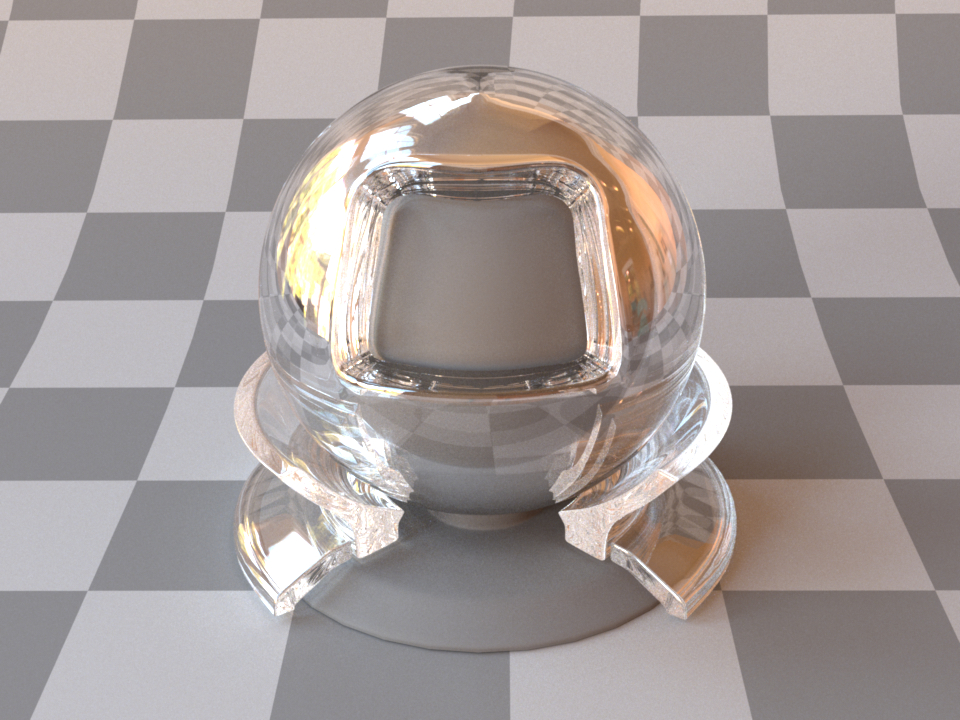
\includegraphics[width=.4\linewidth]{img/dielectric_diamond.jpg}
		&
		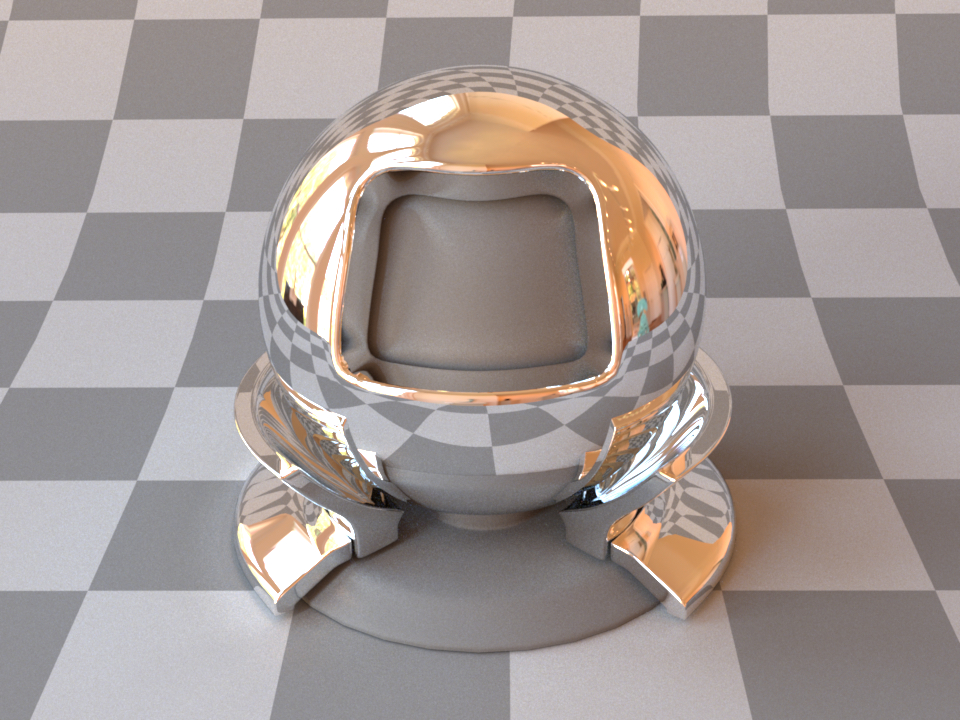
\includegraphics[width=.4\linewidth]{img/conductor_aluminium.jpg}
	\end{tabular}
	\caption{A preview of a dielectric (diamond, left) a  conductor (aluminium, right) rendered in Mitsuba2~\cite{mitsubaWeb}}
	\label{fig:compare_dielectric_conductor}
\end{figure}

While this is a matter of simply computing the Fresnel equations, the practice is more complicated as most of the commonly seen materials are not perfectly smooth. They may be created rough on purpose or slight imperfections due to the manufacturing errors cause that the surfaces are generally rough.

\subsection{Microfacet theory}
With that in mind, the \emph{microfacet theory} was developed by \citet{cook1982reflectance} to address this aspect and provide a theoretical representation of the rough surfaces.

The main idea is that a rough surface consists of the \emph{microfacets} -- a collection of very small surfaces distributed statistically throughout the whole underlying \emph{macrosurface}. The aggregate behavior of the computed values for each of these microfacets determines the final scattering. An example of such distribution is shown in \autoref{fig:microfacets}.

\begin{figure}[h]
	\centering
	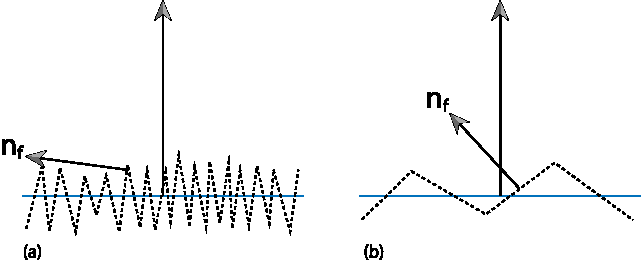
\includegraphics[width=.8\linewidth]{img/microfacets.pdf}
	\caption{A demonstration of a very rough (left) and a relatively smooth (right) microfacet distribution~\cite{pharr2016physically}}
	\label{fig:microfacets}
\end{figure}

As these microfacet computations are local, we need to consider the possibility that they might obscure each other. Three main aspects are accounted for:
\begin{description}
	\item[Masking] Microfacet is not visible from the viewer
	\item[Shadowing] Microfacet is not reachable from the light source
	\item[Interrecflection] Bounces between the microfacets
\end{description}

Many variations to the Cook-Torrance model have been developed, such as its predecessor Torrance-Sparrow~\cite{Torrance1967TheoryFO} or Oren-Nayar~\cite{oren1994generalization} for diffuse reflectance.

In this thesis, we focus on the distribution functions of the microfacets as they are ultimately the deciding factor of the rough surface look. A nice comparison of the three commonly used microfacet distributions --- \emph{Phong}, \emph{Beckmann} and \emph{GGX} -- along with their distribution functions, masking functions and sampling equations can be found in the \citet{walter2007microfacet}. As the exact formulations of those three methods are not a necessity for this thesis, we provide only a brief overview for each of them and an illustrative comparison between the GGX and the Beckmann of the same roughness in 
\autoref{fig:ggx_beckmann}.

\paragraph{Phong}

Even though the Phong distribution is purely empirical (not physically based), it is still quite popular choice for the microfacet distribution as it is simple to implement and provides sufficient results.

\paragraph{Beckmann}

The Beckmann distribution~\cite{beckmann1987scattering} is already physically based and for a long time has been considered the best solution to the rough surfaces as it is based on the Gaussian roughness. However, with the parameters set appropriately, it still provides the results very similar to the Phong distribution.

\paragraph{GGX}

The GGX distribution~\cite{walter2007microfacet} was introduced as an improvement over the Beckmann's solution for some cases. It maintains stronger tails, thus better shadowing and is based on the measured data of the real rough materials.

\begin{figure}[h]
	\centering
	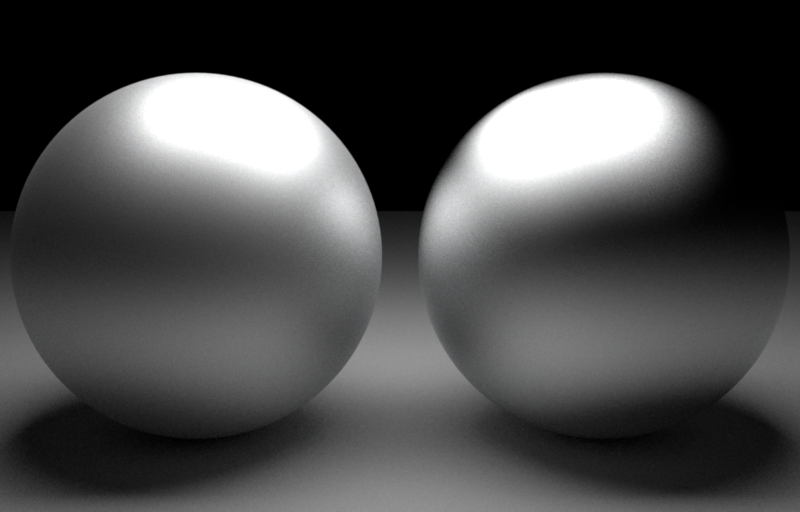
\includegraphics[width=.8\linewidth]{img/ggx_beckmann.png}
	\caption{A rough aluminium sphere with the GGX distribution (left) compared to its Beckmann equivalent (right) rendered  in Mitsuba2}
	\label{fig:ggx_beckmann}
\end{figure}

\section{Polarization}
\label{sec:polarization}

Similarly to all kinds of the electromagnetic radiation, the light also propagates through space as a wave. The oscillation direction of this wave neither defines nor modifies the color of the light but it makes the light behave differently upon an interaction with certain materials. \autoref{fig:oscillation} explains the different directions of a wave.

\begin{figure}[h]
	\centering
	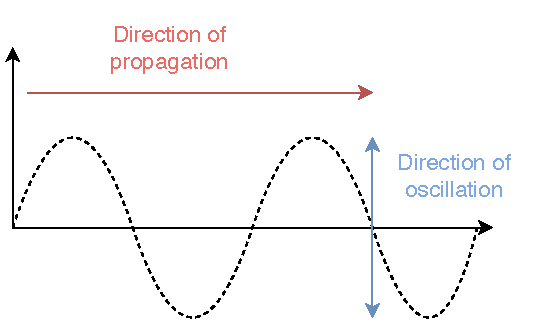
\includegraphics[width=.6\linewidth]{img/oscillation.pdf}
	\caption{Demonstration of the direction of oscillation and the direction propagation}
	\label{fig:oscillation}
\end{figure}

In the light's natural state (sun, common light bulb), the directions of its oscillation are arbitrary --- such light is called \emph{unpolarized}. The \emph{polarized} light maintains a restricted direction of oscillation and it is a result of a \emph{polarization} process. Note that the light is often only partially polarized as the restriction of the direction does not have to be perfect and allows some variations.

Depending on the shape of their electric fields, we distinguish three types of polarization which are demonstrated in \autoref{fig:polar_types}.

\begin{figure}[h]
	\centering
	
\includegraphics[width=.7\linewidth]{img/polar_types.png}
	\caption[polar types]{An illustrative demonstration of the different types of polarization \footnotemark}
	\label{fig:polar_types}
\end{figure}
\footnotetext{\url{http://hyperphysics.phy-astr.gsu.edu/hbase/phyopt/polclas.html}}

To create a linearly polarized light, one may put a dielectric object in the direction of propagation of an unpolarized light. Due to the optical properties of the dielectrics, the reflected and the transmitted light will be polarized proportionally to the angle of the incidence. The angle at which the reflected light is perfectly polarized is called the \emph{Brewster's angle}~\cite{brewster1815laws}. It is computed by the following formula:

\begin{equation}
\theta=arctan(\frac{n_2}{n_1})
\end{equation}
, where $n_1$ is the IOR of the incident medium and $n_2$ of the transmitted medium.

In this case, we distinguish two types of the linearly polarized light depending on their relative orientation to the incident plane. The reflected light is called \emph{p-polarized} as its oscillation is parallel to the plane of incidence. The transmitted light is called \emph{s-polarized} as its oscillation is perpendicular (from the German word) to the plane of incidence. Both are shown in \autoref{fig:brewster}.

\begin{figure}[h]
	\centering
	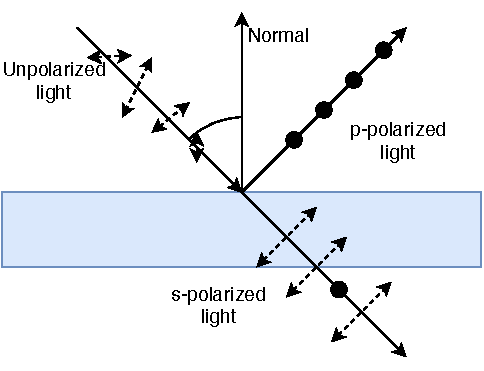
\includegraphics[width=.7\linewidth]{img/brewster.pdf}
	\caption{Prefectly p-polarized reflected and partially s-polarized light refracted from a dielectric interface at the Brewster's angle}
	\label{fig:brewster}
\end{figure}


The principle of Brewster's angle is used in a material called the \emph{polarizer}. As the name suggests, it polarizes the light, restricting its direction of oscillation accordingly to the specifics of the polarizer. If the light that passes through the polarizer is of the opposite (perpendicular) direction to the polarizer's transmission orientation, it won't let it through and no light is visible. \autoref{fig:polarizer} illustrates the effects of a polarizer.

\begin{figure}[h]
	\centering
	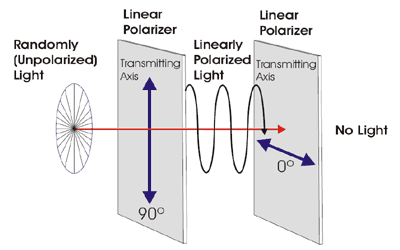
\includegraphics[width=.6\linewidth]{img/polarizer.png}
	\caption[nikon]{Unpolarized light passes through a vertical polarizer $\rightarrow$ linearly vertically polarized light passes through a horizontal polarizer $\rightarrow$ no light\footnotemark}
	\label{fig:polarizer}
\end{figure}
\footnotetext{\url{https://www.apioptics.com/about-api/resources/visible-light-linear-polarizer/}}

This property is frequently incorporated in the sunglasses or camera filters to reduce the glare of the sun reflected from a horizontal surface. The reflected p-polarized light goes through a polarizer with a perpendicularly oriented transmission axis which consequently eliminates the incoming light. The effect of a polarizing filter is shown in \autoref{fig:polarizer_nikon}.

\begin{figure}[h]
	\centering
	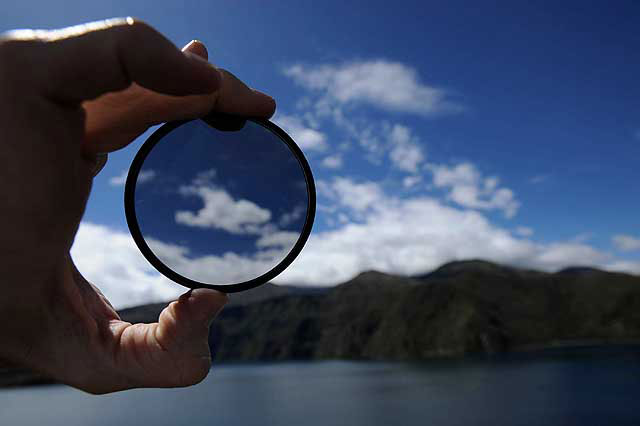
\includegraphics[width=.7\linewidth]{img/polarizer_nikon.jpg}
	\caption[nikon]{Polarizing filter by Nikon\footnotemark}
	\label{fig:polarizer_nikon}
\end{figure}
\footnotetext{\url{https://www.nikonusa.com/en/learn-and-explore/a/tips-and-techniques/polarizing-filters-add-pow-to-pictures.html}}

As the polarization is a vast topic, we do not need to go into further detail for the purposes of this thesis. If the reader wishes to learn more, please refer to a scientific literature, for example \citet{kliger2012polarized}

\subsection{Polarization in rendering}
The integration of the polarization in the rendering process is quite rare as only a few scenarios display the effects of the polarization and one must implement quite complex behavior of the radiation waves to the spectral rendering. However, renderers such as Mitsuba2 or ART fully track the polarization state of light when needed. The implementation covered by this section is already in Mitsuba2~\cite{mitsubaWeb}.

The polarization state is represented by \emph{Stokes vector} --- a 4-dimensional quantity that fully parameterizes the elliptical shape of the light's electric field for each wavelength separately. The information stored in the Stokes vectors is explained in \autoref{fig:stokes}.

\renewcommand\thesubfigure{\arabic{subfigure}}
\begin{figure}
	\centering
	\begin{tabular}{cc}
		\begin{subfigure}
			{0.4\textwidth}\centering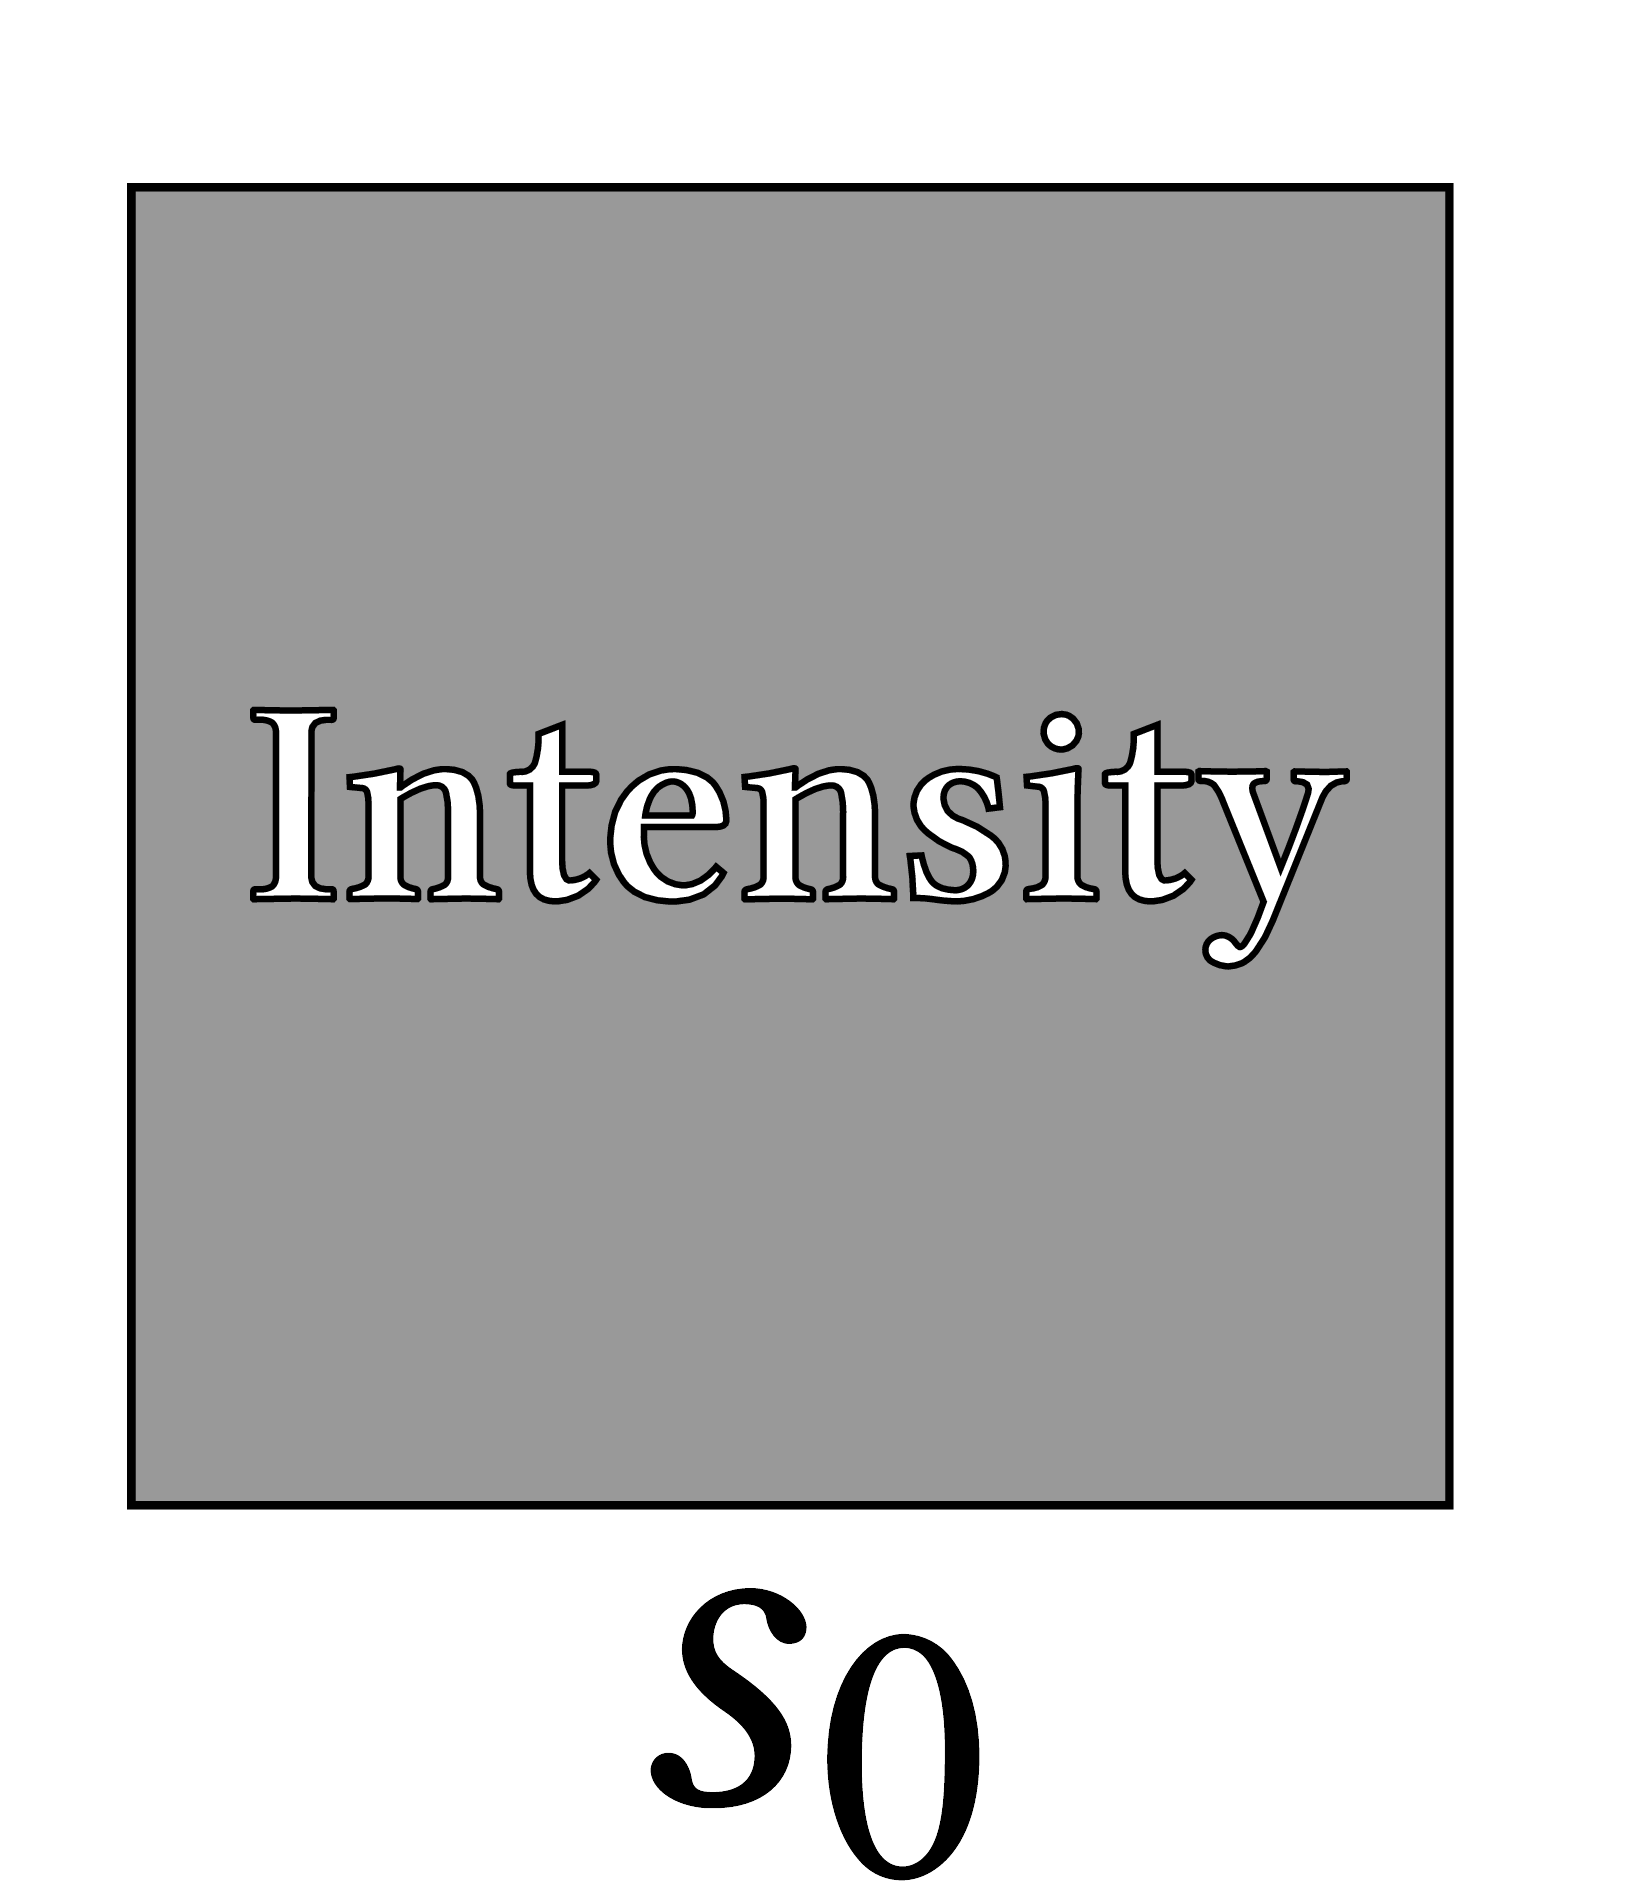
\includegraphics[width=\linewidth]{img/stokes1.png}
			\caption{Radiance - no polarization}
		\end{subfigure}
		&
		\begin{subfigure}
			{0.4\textwidth}\centering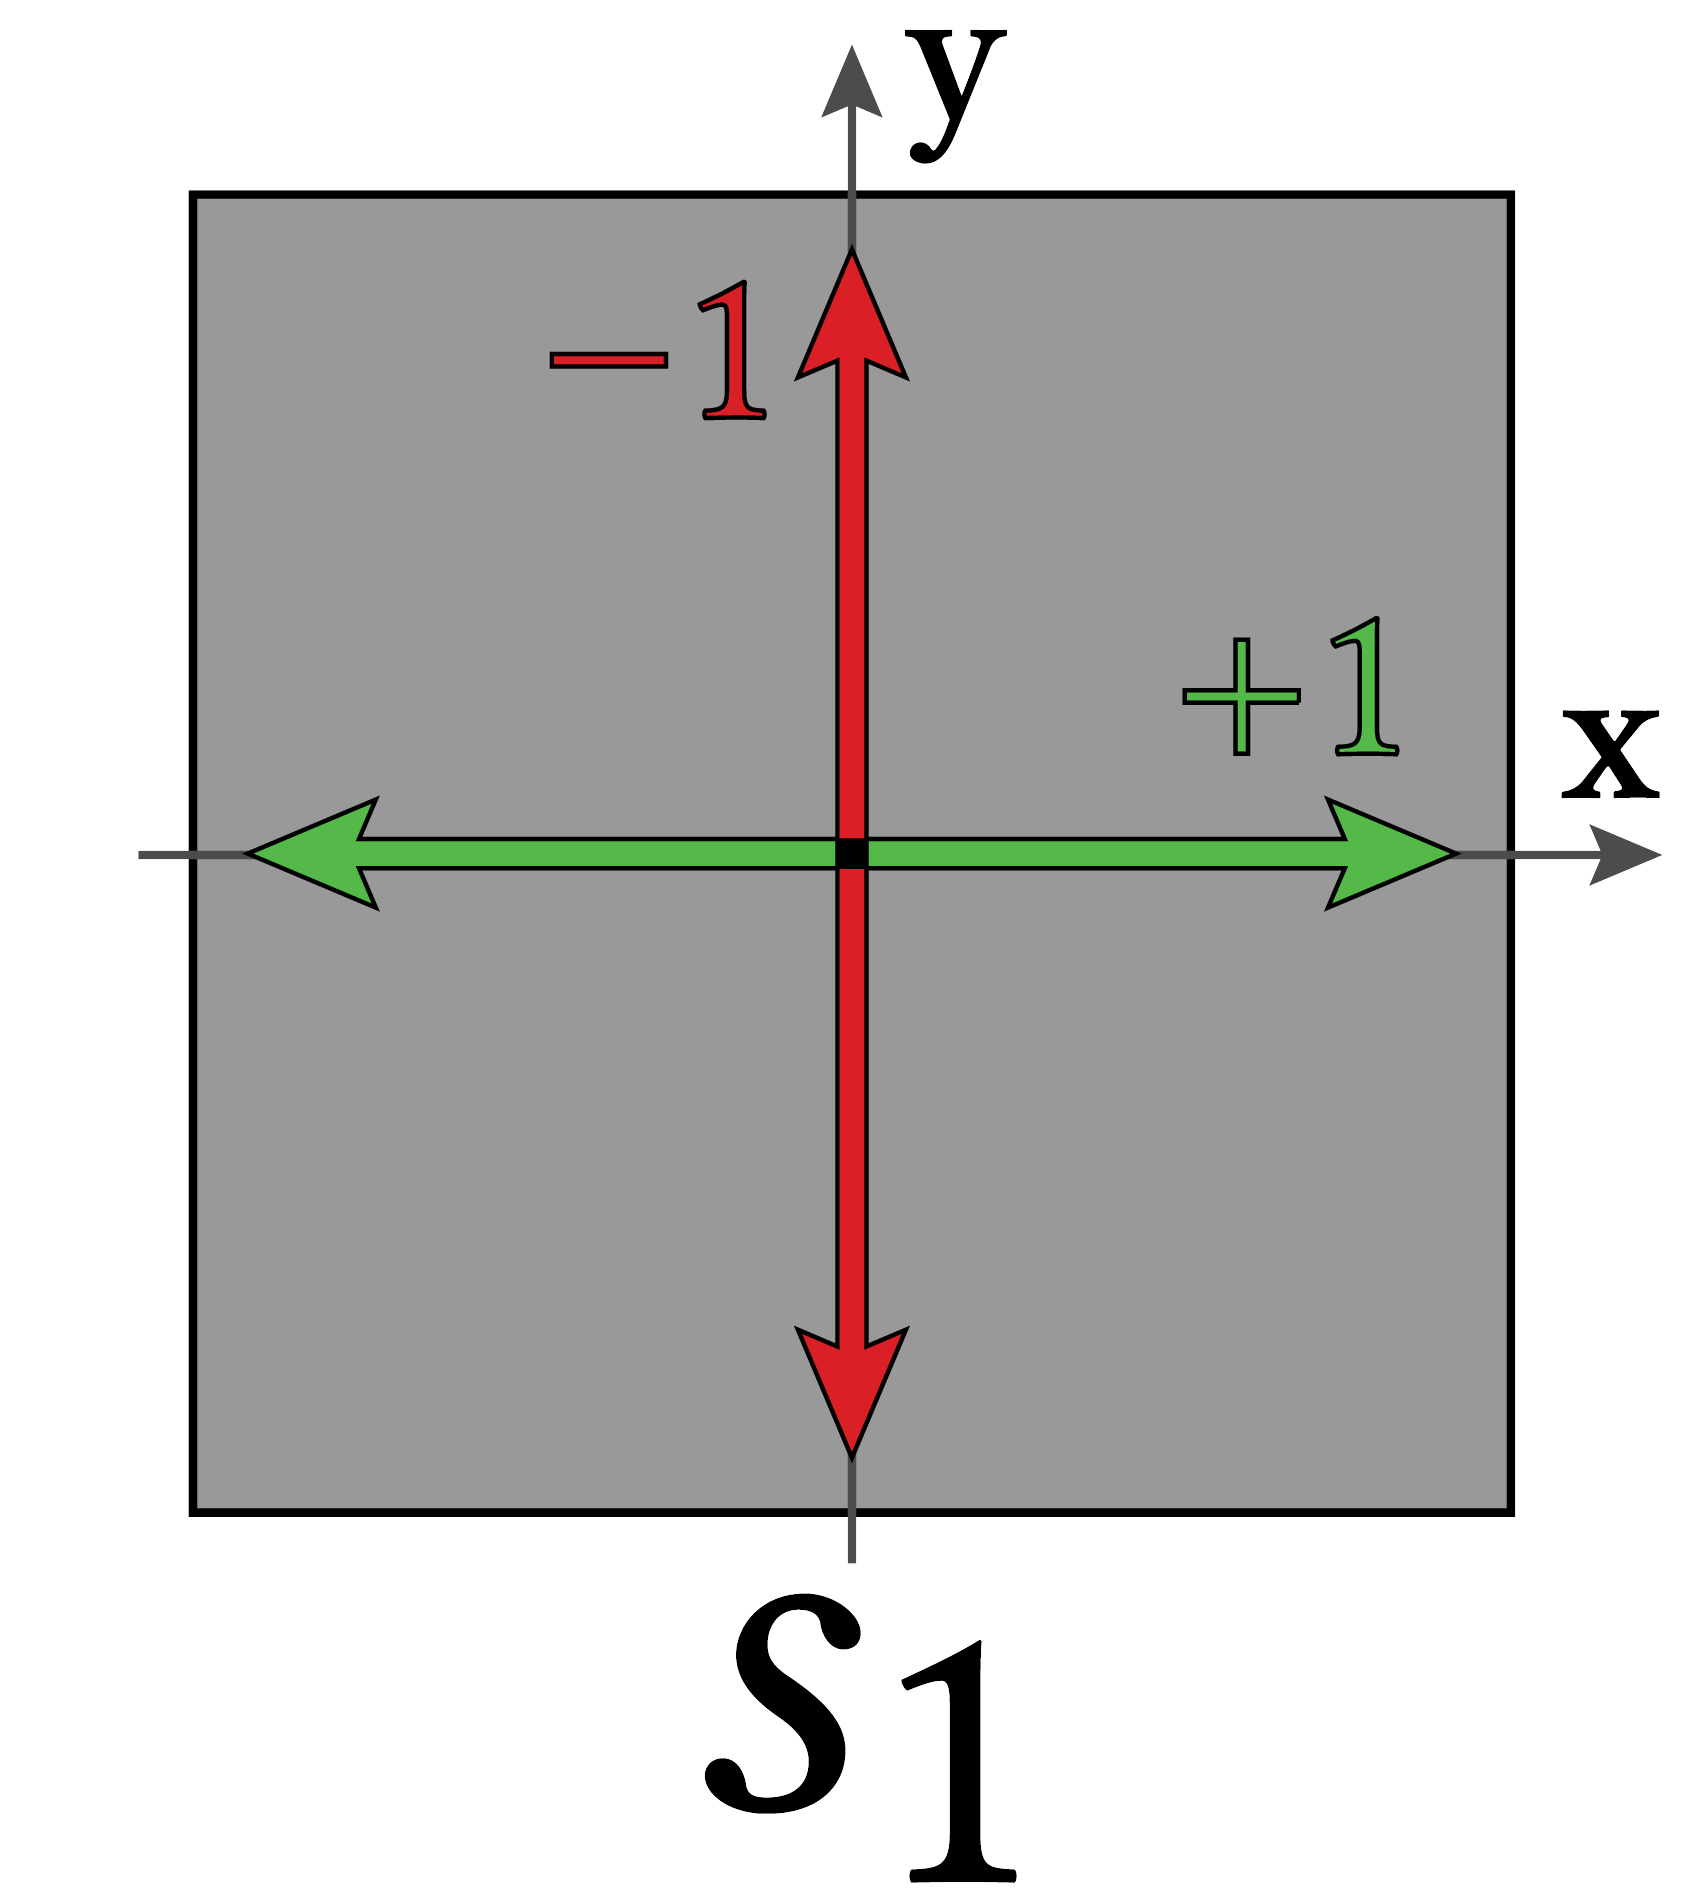
\includegraphics[width=\linewidth]{img/stokes2.png}
			\caption{Horizontal vs. vertical polarization}
		\end{subfigure} \\
		\begin{subfigure}
			{0.4\textwidth}\centering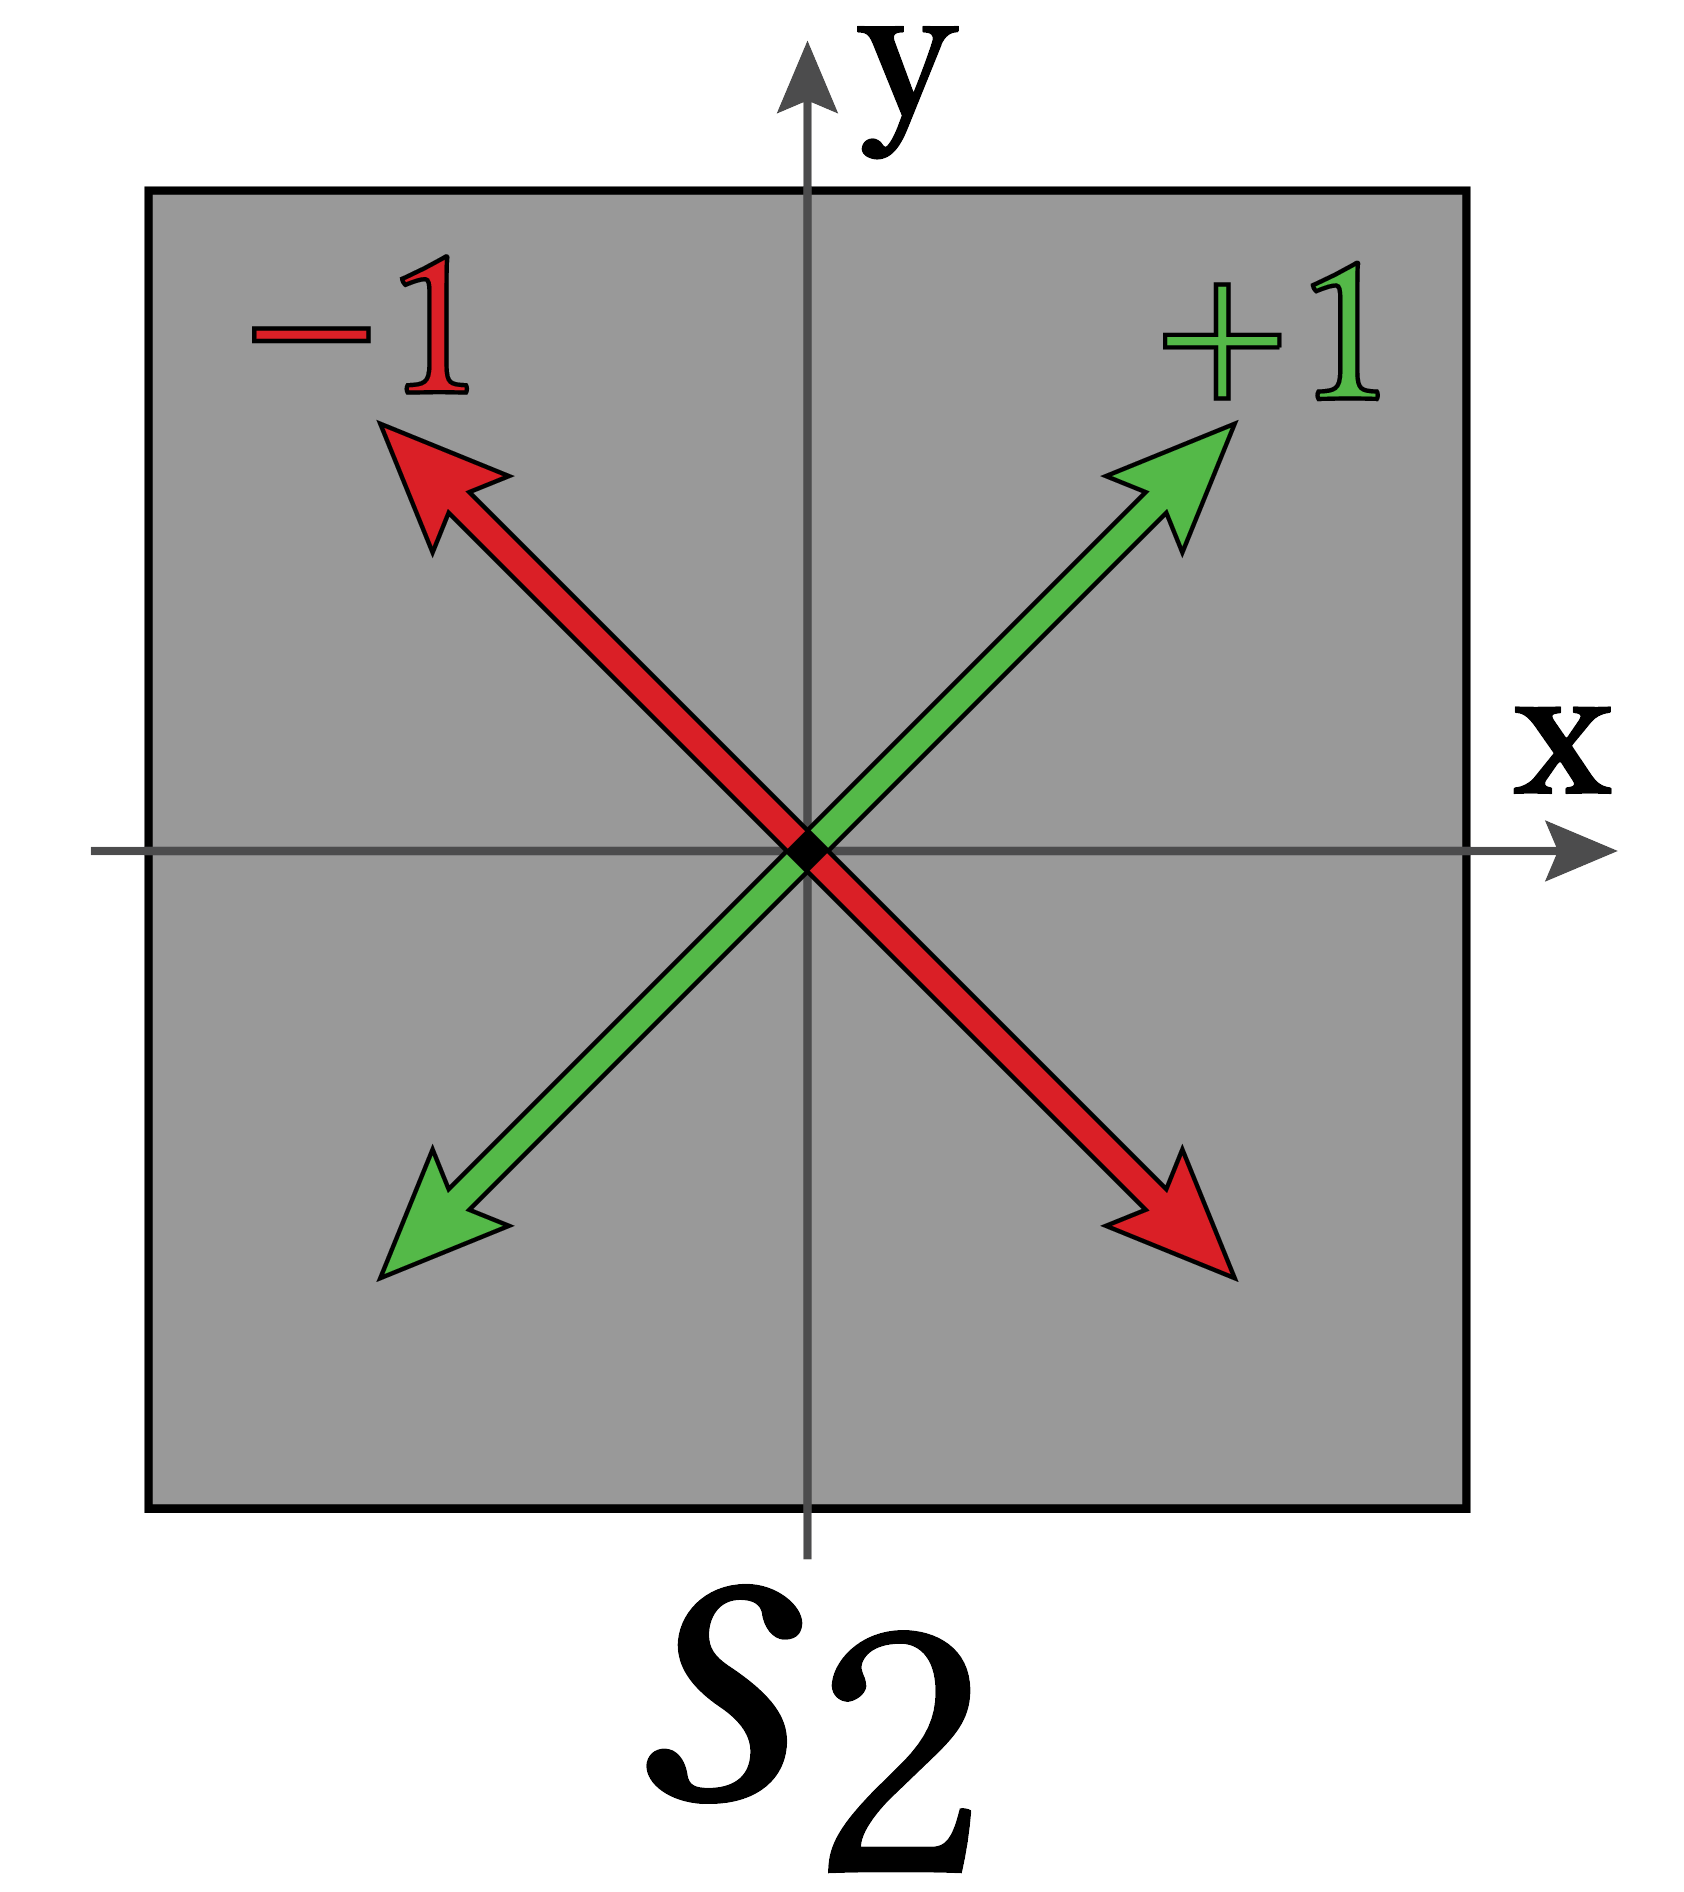
\includegraphics[width=\linewidth]{img/stokes3.png}
			\caption{Diagonal polarization}
		\end{subfigure} 
		&
		\begin{subfigure}
			{0.4\textwidth}\centering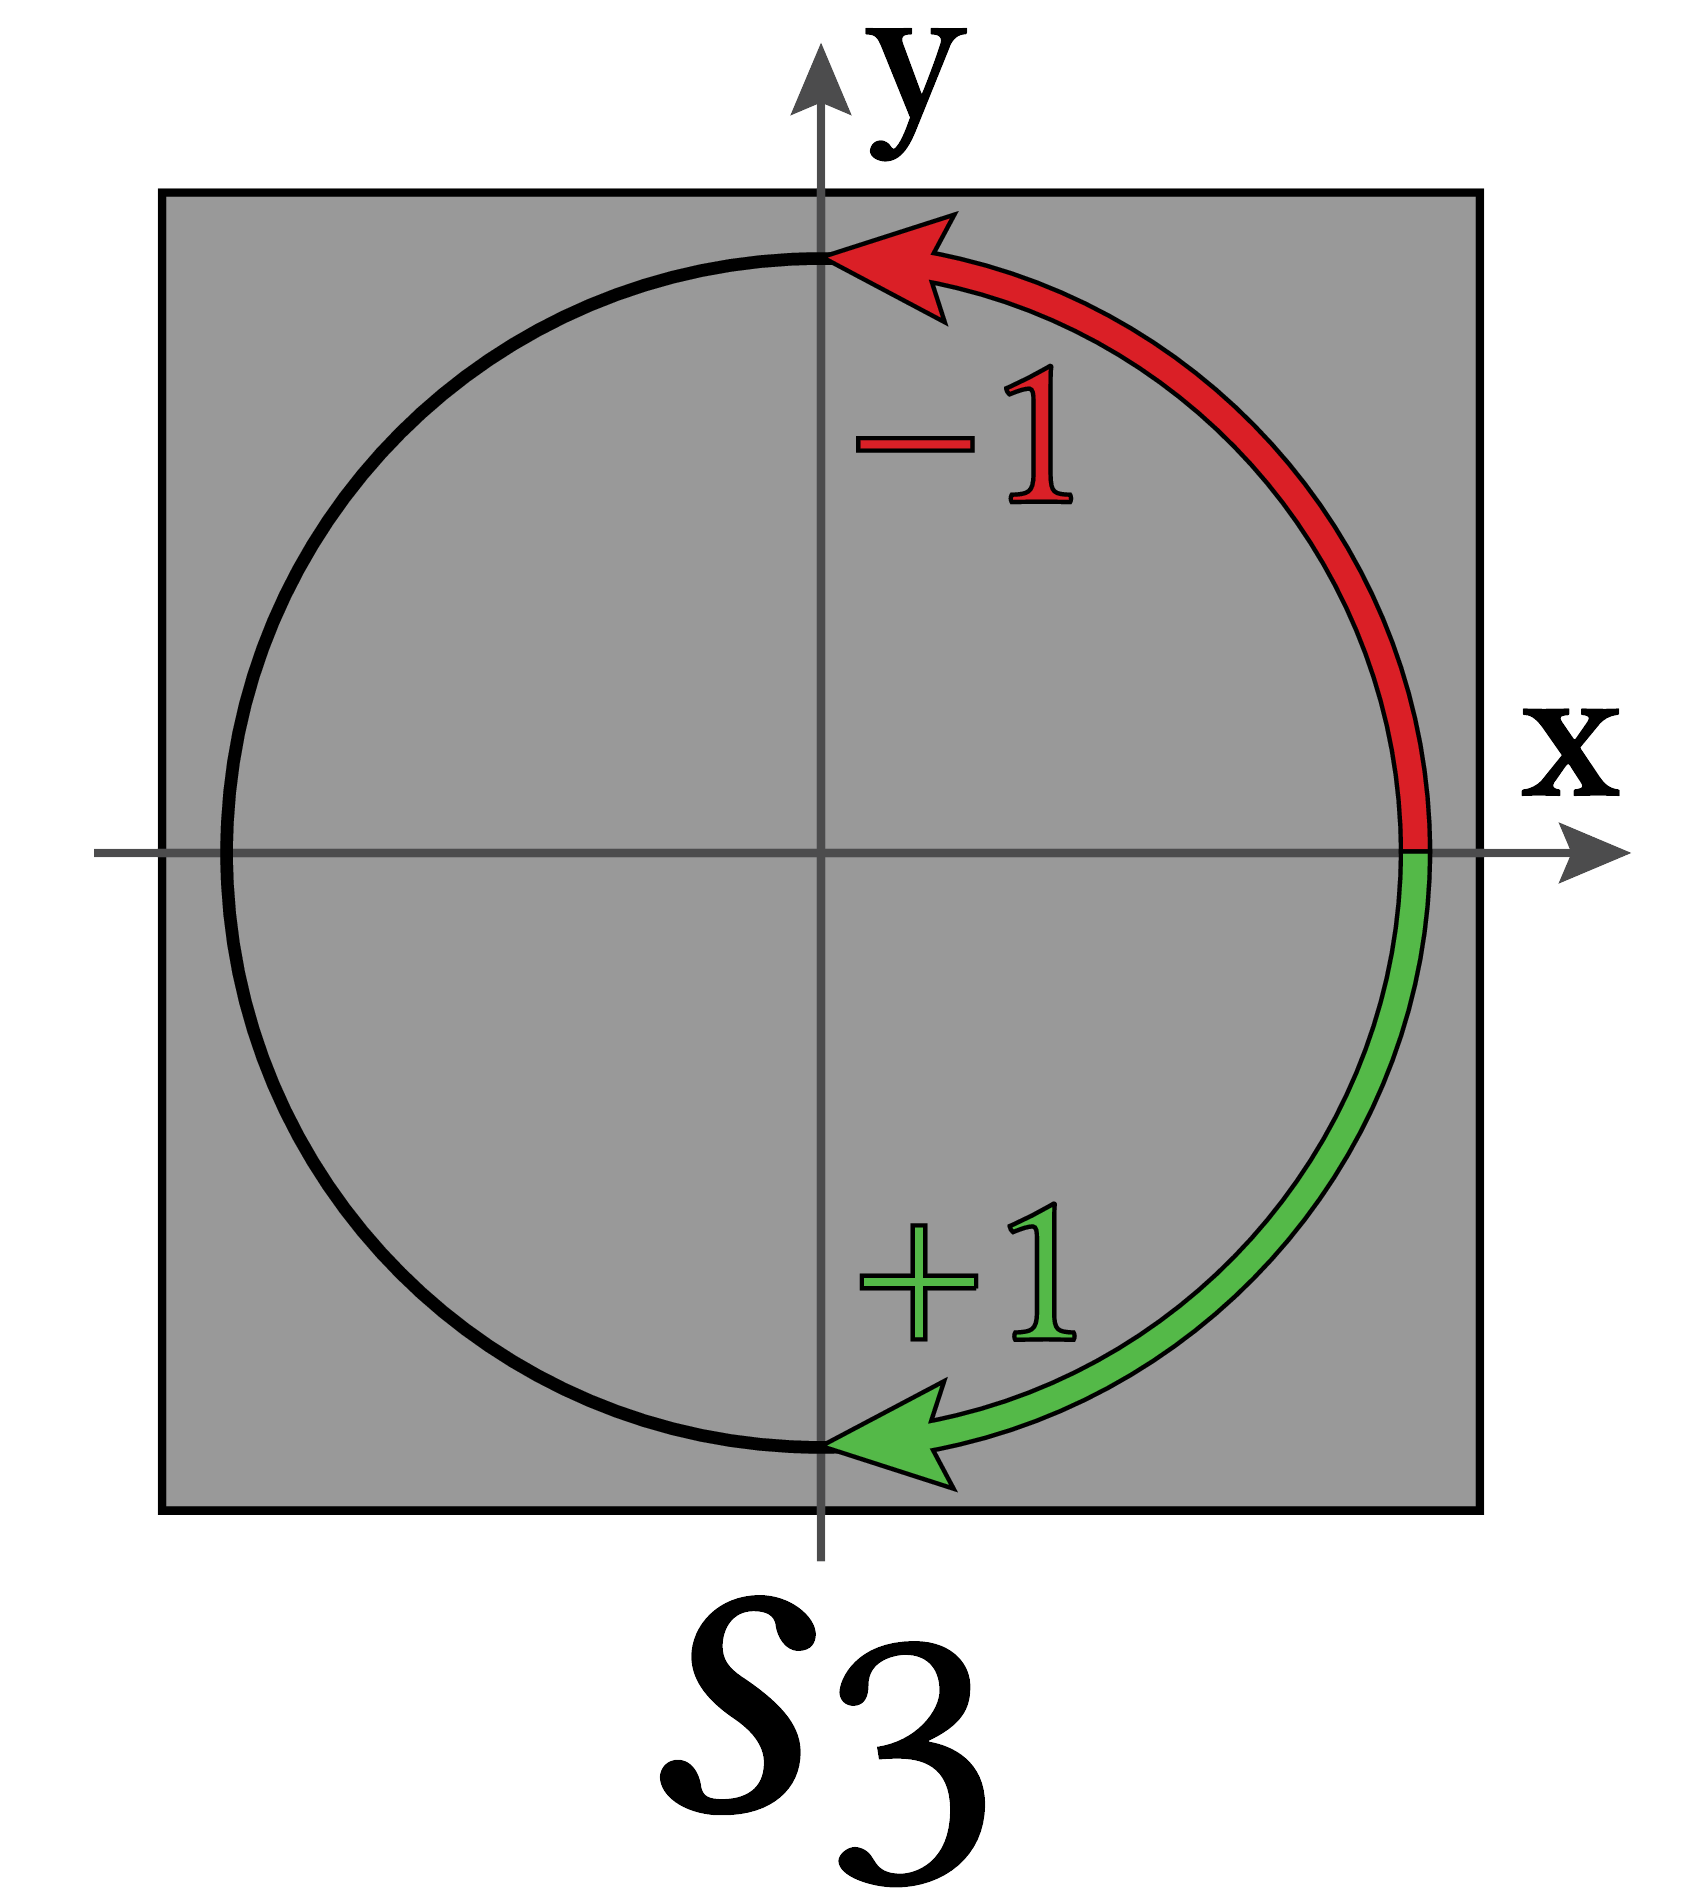
\includegraphics[width=\linewidth]{img/stokes4.png}
			\caption{Left vs. right circular polarization}
		\end{subfigure}
	\end{tabular}
	\caption{Different information carried by the Stokes vector}
	\label{fig:stokes}
\end{figure}

As we have the polarization states properly represented and we can track them throughout the rendering process, the next step is to determine the affects to these states upon a surface interaction. A transformation between the incoming state and the outgoing state is represented by the \emph{Mueller matrix} $M \in \R^{4x4}$. Due to the adjustments to all interactions in the light transport, we also generalize the BSDF $f_r(\lambda,\omega_i,\omega_o)$ to the polarized pBSDF $M(\lambda,\omega_i,\omega_o)$.

If the  reader is curious about the complications this implementation brings and their solutions, he may want to look into the details of Mitsuba2 in \citet{nimier2019mitsuba}. Nevertheless, they are not crucial for the purposes of this thesis and we purposely skip them.

\section{Dispersion}

Generally, the IOR of a dielectric at least slightly varies for different wavelengths (e.g. glass has IOR between 1.5 and 1.6). This causes that the polychromatic light is split into its spectral components upon an intersection with such materials. As each wavelength is slightly shifted, a rainbow effect can be perceived --- this phenomenon is called the \emph{dispersion}. In the nature, it can be frequently seen when light passes through liquids (sun through rain). For the scientific purposes, several variations of a device called the dispersive prism~\ref{fig:dispersion} have been created for this purpose. 

\begin{figure}[h]
	\centering
	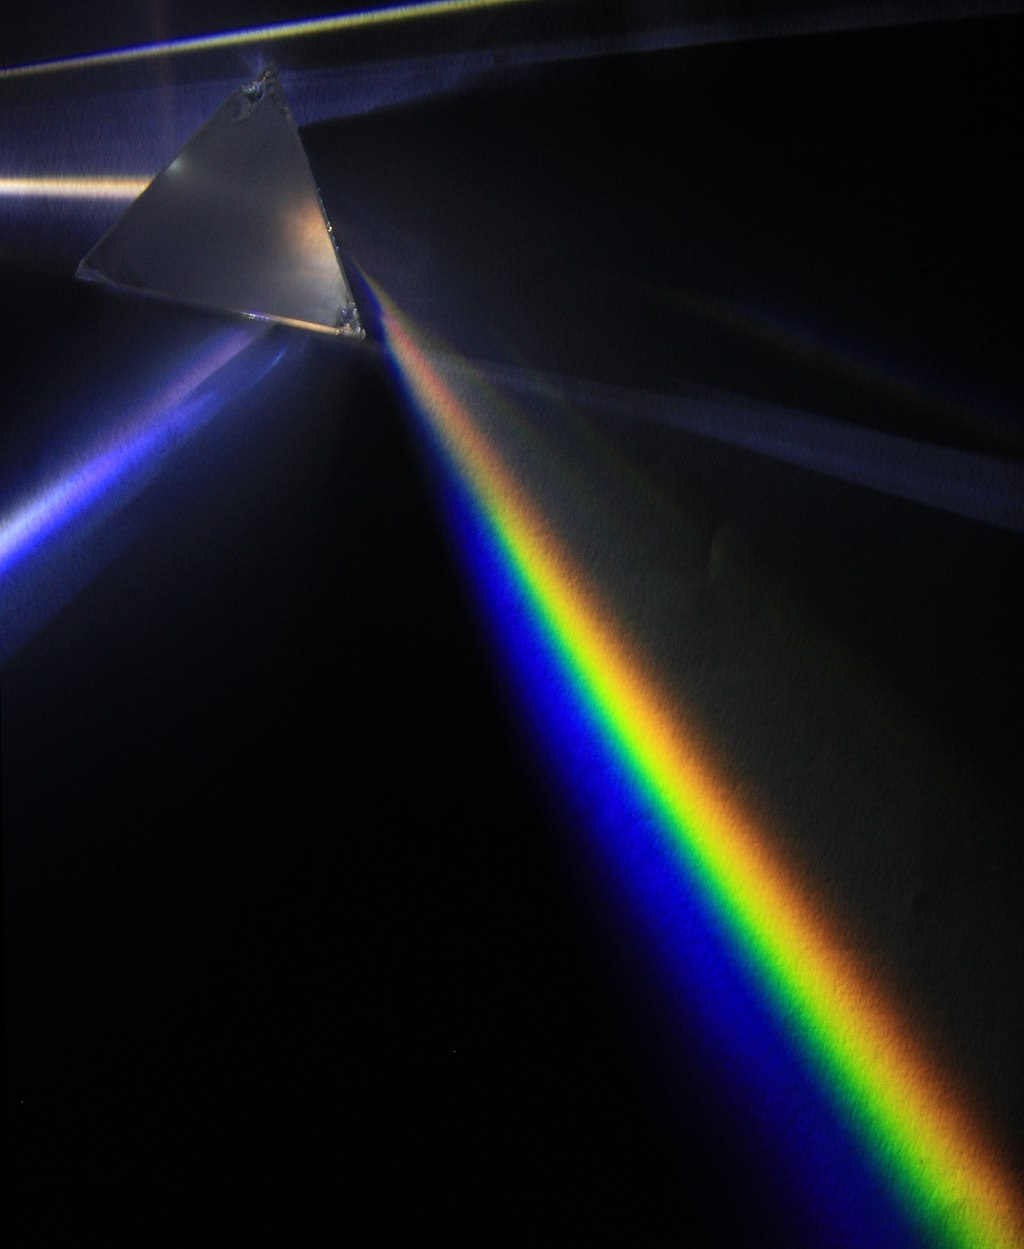
\includegraphics[width=.6\linewidth]{img/dispersion.jpg}
	\caption[nikon]{Photograph of a dispersive prism\footnotemark}
	\label{fig:dispersion}
\end{figure}
\footnotetext{\url{https://en.wikipedia.org/wiki/Dispersive_prism}}

In the computer graphics, even though it is possible to simulate the dispersion in the tristimulus rendering, it is insufficient and the obvious choice would be to use the spectral rendering as it already contains most of the information about the tracking of the wavelengths. 

The missing part is the representation of the varying IOR --- currently, the widely used method is called \emph{Sellmeier approximation}~\cite{wilkie2002tone}. Then, we have to add the ability to track the possibly dispersed monochromatic rays upon a surface interaction of a single polychromatic ray, i.e. create extra samples that were unnecessary before.

\section{Iridescence}
\label{sec:irid}

It is quite common that some objects in the nature exhibit an interesting behavior where the hue of their surface graudally changes with the viewing angle and the illumination angle, such as butterfly wings, soap bubbles, oil etc. This phenomenon is called \emph{iridescence} or \emph{goniochromism} and is caused by a large amount of interferences between the light waves and their consequent scattering depending on their wavelength which produces a rapid change in colors~\cite{belcour2017practical}.

We distinguish two main types of the iridescence:

\begin{description}
	\item[Microscopic structures] Reflections from structures of a size similar to the wavelength (e.g. peacock feathers)
	\item[Thin film] Light interaction with a thin film of a size similar to the wavelength (e.g. soap bubble)
\end{description}

An example of both can be seen in \autoref{fig:iridescent_example}.

\begin{figure}
	\centering
	\begin{tabular}{cc}
		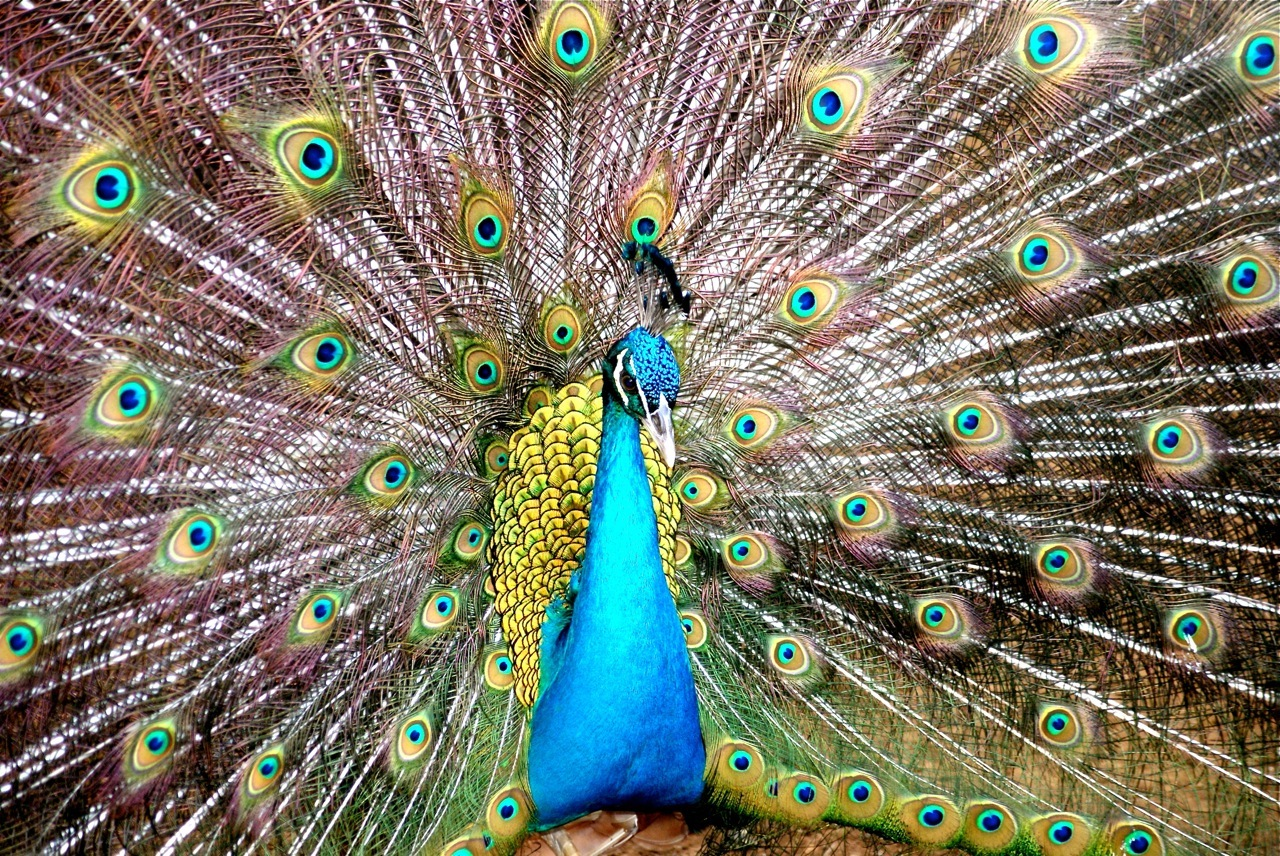
\includegraphics[width=0.4\linewidth]{img/iridescent_peacock.jpg}
		&
		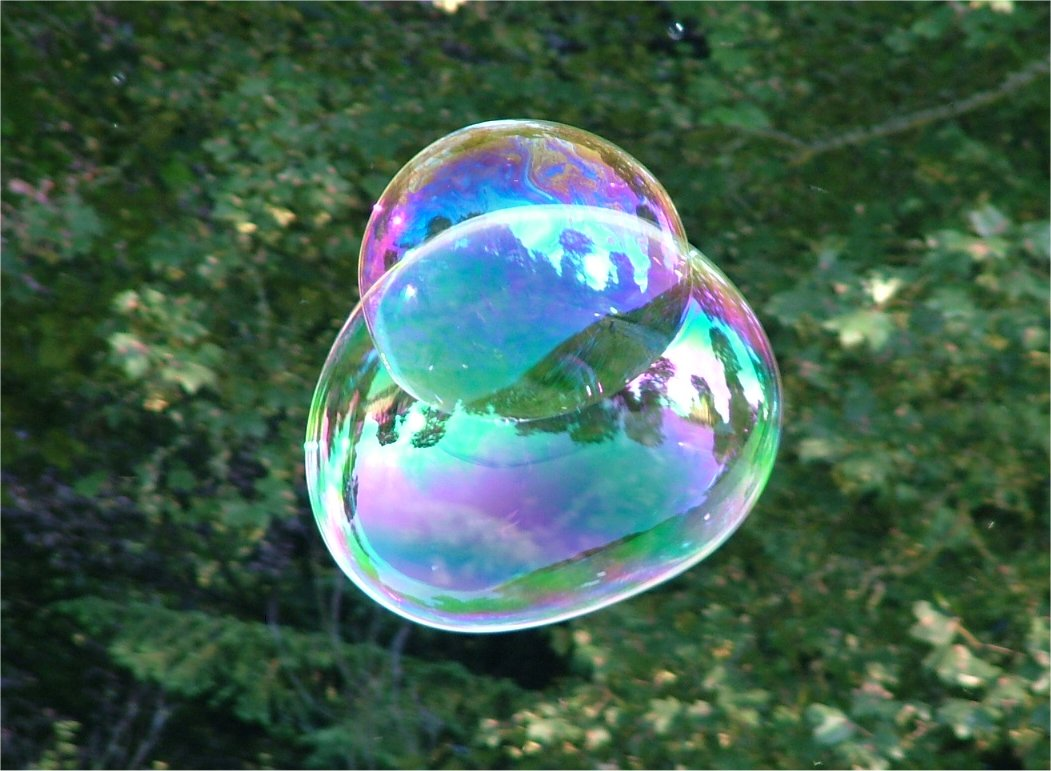
\includegraphics[width=0.4\linewidth]{img/iridescent_soap.jpg}
	\end{tabular}
	\caption[Irid example]{Structural iridescence of the peacock feathers (left) and the thin-film light interference in a soap bubble (right)\footnotemark}
	\label{fig:iridescent_example}
\end{figure}
\footnotetext{\url{https://en.wikipedia.org/wiki/Iridescence}}

In this thesis, we focus on the thin-film interference as it is nicely described as a physical process and it is already incorporated in Mitsuba~\cite{belcour2017practical}. From now on, by iridescence we mean the thin-film interference until told otherwise.

First, look at the light interactions inside the membrane of a soap bubble in \autoref{fig:soap}. The light strikes at the surface of the film, based on the angle it can be either reflected or transmitted. The transmitted light very quickly strikes the bottom boundary of the soap bubble (as it is very thin) and again can be reflected and/or refracted. As the film is a few hundreds of nanometers thick, this repeats with a great frequency and, as you can see, the light transmitted from the upper boundary can easily interfere with the light reflected from the lower boundary.

\begin{figure}[h]
	\centering
	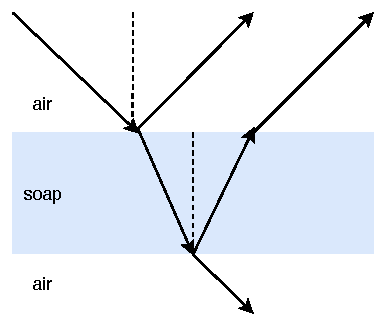
\includegraphics[width=.6\linewidth]{img/soap.pdf}
	\caption{A cross-section of a light interaction with a soap bubble}
	\label{fig:soap}
\end{figure}

An obvious observation is that the iridescence is also dependent on the thickness of the interacting layer - as the thickness increases, the transmission of the light takes longer time which consequently causes a lot less interferences. The difference between two variously thick films is displayed in \autoref{fig:irid_heights}.

\begin{figure}[h]
	\centering
	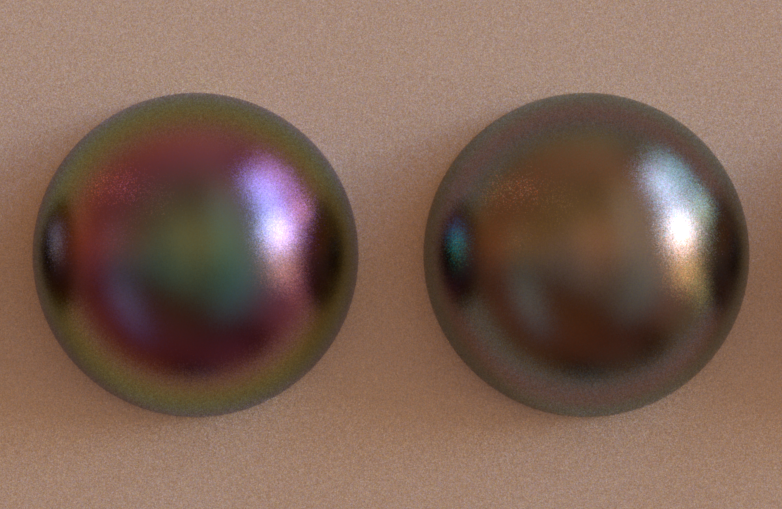
\includegraphics[width=.6\linewidth]{img/irid_heights.png}
	\caption{Two identical rough conductors with differently thick film layers on top of them: 550nm (left) vs. 1500nm (right) rendered in Mitsuba2}
	\label{fig:irid_heights}
\end{figure}

\subsection{Iridescence in rendering}

Based on the \citet{belcour2017practical}, we overview the computational process of the iridescence caused by a thin film on top of a rough material. We purposely avoid the exact formulations of the equations as these would be unnecessarily complicated to explain and it is sufficient to comprehend the basics in order to evaluate the correctness of the computation. For more details, the interested reader is referred to the \citet{belcour2017practical}.

Essentially, this procedure computes an iridescence term of the thin film layer that is plugged into the BSDF of the rough base surface:

\begin{enumerate}
	\item Compute the reflected and the transmitted values of the Fresnel equations for the IOR of the film and the IOR of the exterior
	\item Compute the optical paths differences between the primary and the secondary light paths
	\item Evaluate the Fresnel phase shift
	\item Determine the term by using the Airy summation for the parallel and perpendicular polarization
\end{enumerate}

\section{Fluorescence}

Curiously, certain materials or substances change their colors with no apparent respect to the illumination color. This behavior is called \emph{fluorescence} and it can be quite commonly observed in the nature, for example in various minerals but also in the living organisms such as fish or arachnids.

The explanation behind this phenomenon is that the molecules of such substances absorb electromagnetic radiation of specific wavelengths and emit back different, usually larger wavelengths. The most eye-catching fluorescence is caused by the absorption of the ultraviolet light which is invisible to the human eye and therefore the fluorescent material might seem to change its color for no reason. An example of a fluorescent calcite is shown in \autoref{fig:calcite}

\begin{figure}
	\centering
	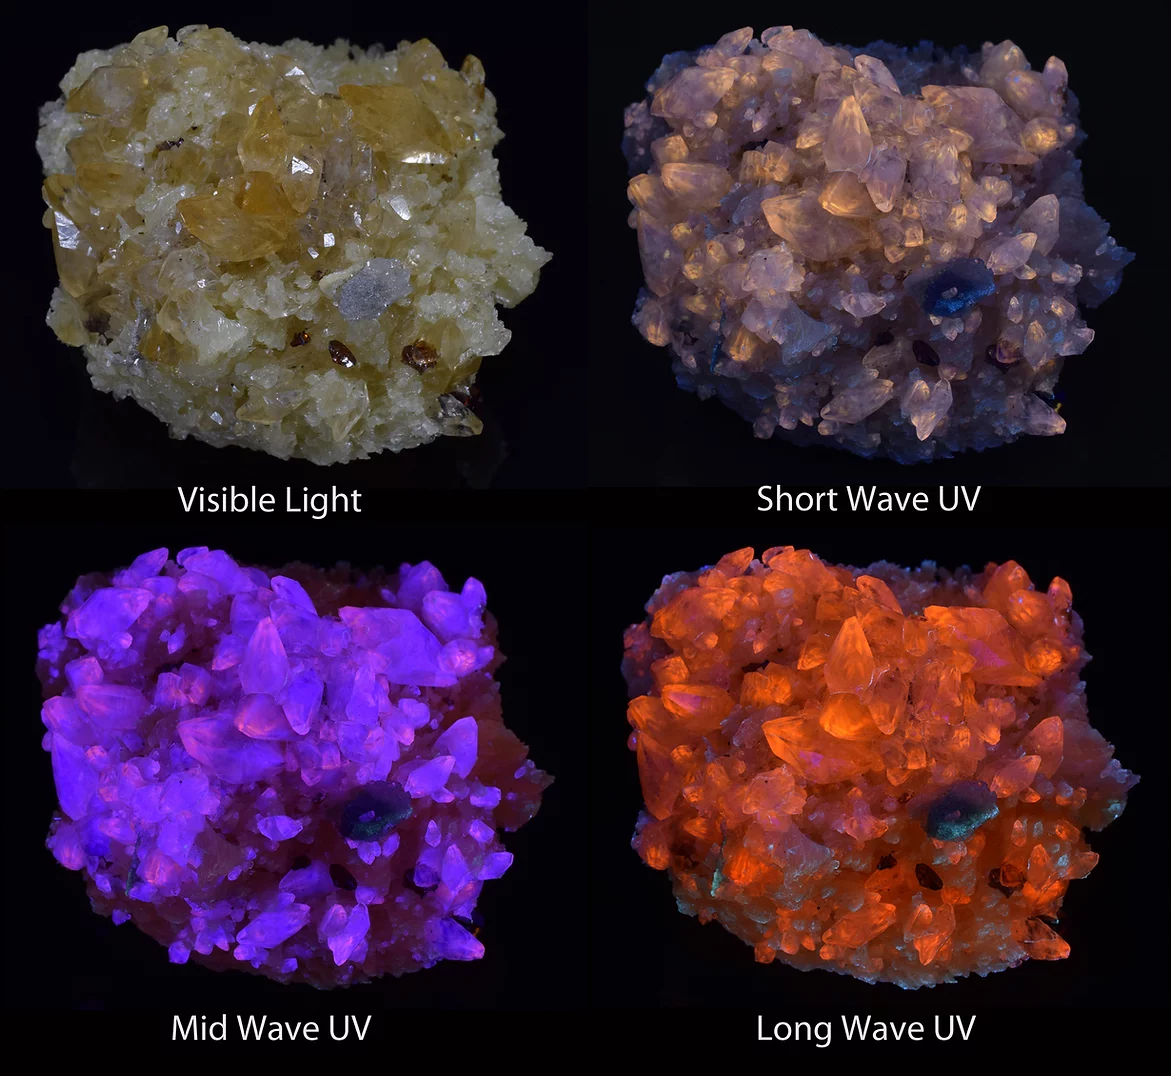
\includegraphics[width=0.8\linewidth]{img/calcite.png}
	\caption[calcite]{Calcite under different lights\footnotemark}
	\label{fig:calcite}
\end{figure}
\footnotetext{\url{https://www.naturesrainbows.com/single-post/2017/11/01/Fluorescent-Multi-Wave-Calcite-from-the-Elmwood-Mine}}

Please note that there is a difference between fluorescence, luminescence and phosphorescence:

\begin{description}
	\item[Luminescence] Natural production of light caused by chemical reactions (no absorption)
	\item[Phosphorescence] Similar to fluorescence but emits light even after the light source is gone
	\item[Fluorescence] The emission stops almost instantaneously after the light source is gone
\end{description}

\subsection{Fluorescence in rendering}
As we are dealing with the wavelengths of a spectrum, the appropriate decision is to extend the spectral rendering to include the fluorescence. Once again, we refer the interested reader to \citet{mojzik2018handling} for the implementation details as we are only covering the fundamental ideas for the purposes of this thesis.

As we've mentioned before, we are in fact shifting the wavelengths of the absorbed spectrum to emit a new one --- this is called \emph{Stokes shift} (shown in \autoref{fig:stokes_shift}) and can be described by \emph{fluorescence response} $\Phi(\lambda_i,\lambda_o)$.

\begin{figure}
	\centering
	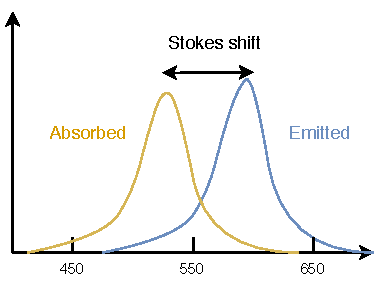
\includegraphics[width=0.7\linewidth]{img/stokes_shift.pdf}
	\caption{Illustration of the Stokes shift}
	\label{fig:stokes_shift}
\end{figure}

The discrete form of a fluorescence response can be represented by \emph{re-radiation matrix} which contains incoming wavelengths on its vertical axis and their corresponding outgoing wavelengths on its horizontal axis. The probability of the shift follows Kasha's rule --- the spectrum distribution of the emitted light should not change, only the intensity of emission spectrum does.

A generalization of the BRDF that includes re-radiation was introduced by \citet{hullin2010acquisition} called \emph{Bi-spectral Bidirectional Reflectance and Re-radiation distribution function (bi-spectral BRRDF)}:
\begin{equation}
f_r((\omega_i,\lambda_i),(\omega_o,\lambda_o))=\frac{d^2L(\omega_o,\lambda_o)}{L(\omega_i,\lambda_i)d\omega_i d\lambda_i}
\end{equation}
and the corresponding \emph{bi-spectral rendering equation}:
\begin{equation}
L(\omega_o,\lambda_o)=\int_{\Lambda}\int_{\Omega}L(\omega_i,\lambda_i)f_r((\omega_i,\lambda_i),(\omega_o,\lambda_o))d\omega_i d\lambda_i
\end{equation}

The topics of this chapter properly explained the appearance phenomena that we are investigating in this thesis. As we covered the basics of their computations as well, we may now proceed with the evaluation process to determine their accuracy.
\chapter{Benchmark}
\label{chap:benchmark}

The main aim of this thesis is to methodically examine the appearance phenomena that are frequently appearing in our day-to-day life but for some reason are still rarely implemented in the modern renderers. However, in the past decade, the interest in the physically realistic renders has grown significantly and the implementations for these phenomena have been introduced. As they are still being consistently improved and integrated into the conventional rendering systems, it is absolutely necessary to have a testing suite which would properly evaluate their accuracy.

We propose a testing suite that contains a minimum number of test scenes which maximally exercise these implementations and an equivalent number of the reference images that we consider to be the ground truth, to our best knowledge. These are encapsulated in an automated workflow, which runs the tests with a single command and shows the results in form of a website. The suite also contains data such as code snippets that should simplify the replication process of these implementations and they can be easily integrated into any standard renderer.

The benchmark follows a few basic principles:

\begin{description}
	\item[Easy to use] The benchmark should provide a user-friendly environment that is comprehensible for an average developer or tester of the rendering features. Therefore, the whole suite is written in Python3 as it is currently one of the most popular scripting languages, it does not need to be compiled and is cross-platform. It also provides CLI command options that are invoke-able via python command.
	\item[Modularity] Each part of the benchmark should be adjustable without the need to heavily modify the other parts. For example, if a new CLI option is to be added, you only need to change the \texttt{/src/arg\_parser.py} file.
	\item[Extensibility] It should be simple enough to extend the capabilities of the benchmark, such as adding new scenes, test case scenarios or even renderers. For example, you don't have to modify any code if you want to add a new scene --- there are structures prepared for this scenario which simply need to be filled.
	\item[Simplicity] The scenes are straightforward, containing only basic and portable geometry, light sources and cameras. This brings two large advantages --- it is fairly easy to replicate them for different renderers and they are simple enough to understand the purpose of each element they contain. Along with the thorough comments, anyone with the basic knowledge acquired in the previous chapters of this thesis should comprehend their meaning.
	\item[Standalone] The benchmark should contain all the data that the potential user would need to properly run or generally use the testing suite. For example, the geometry that is included in the scenes can be found in the \texttt{/data/common/} folder.
\end{description}

\section{Framework}

First of all, we take a look into the framework of the benchmark suite and its structure. The file organization is demonstrated in \autoref{fig:framework} and the following sections describe each major subsection of it.

\begin{figure}
	\centering
	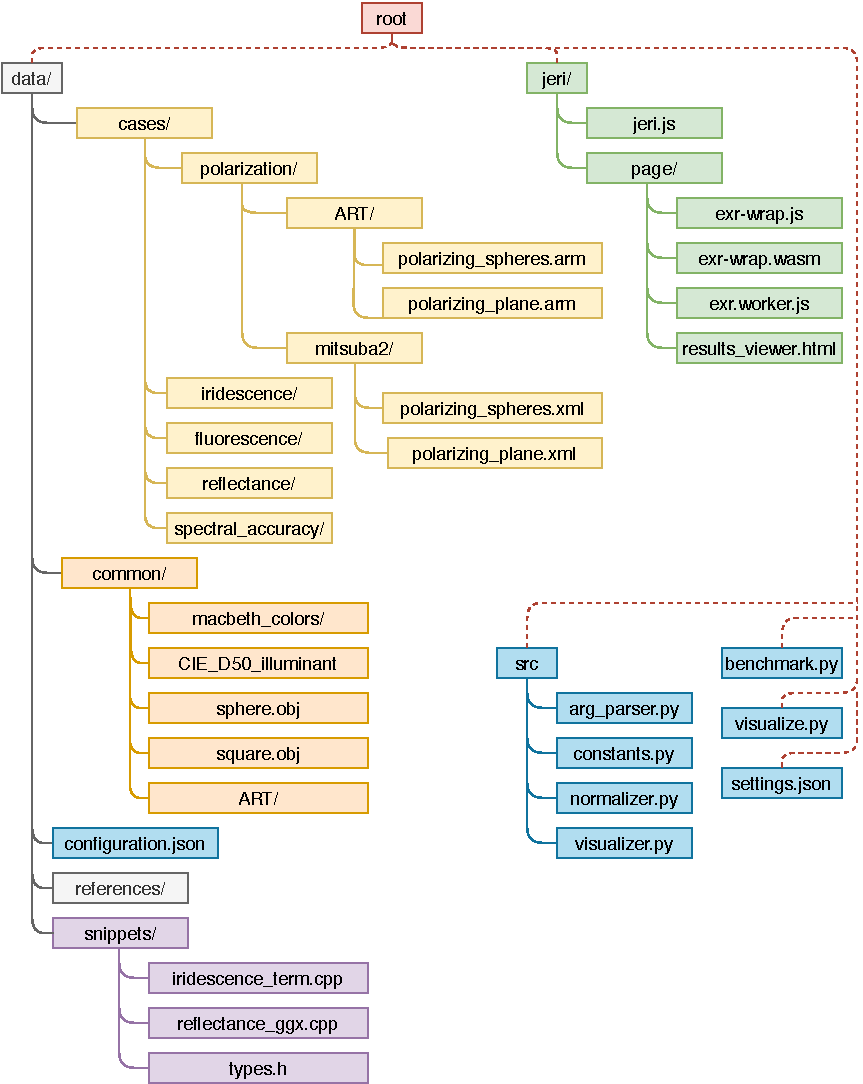
\includegraphics[width=\linewidth]{img/framework.pdf}
	\caption{File organization of the benchmark}
	\label{fig:framework}
\end{figure}

\subsection{Code}

An automated workflow simplifies the benchmark process and ensures that the user is working with the benchmark correctly. The suite consists of several files to accommodate the principle of modularity:

\begin{description}
	\item[src/arg\_parser.py] Parses the CLI arguments and the \texttt{settings.json} file and fills its variables accordingly.
	\item[src/constants.py] Simply contains the constants that are used in other scripts.
	\item[src/normalizer.py] Normalizes the names of the resulting images after the benchmark ends, as each renderer might have unique naming conventions. It is used only in corner cases.
	\item[src/visualizer.py] Runs a HTTP server which is required by jeri.io to upload EXR images and opens the website with the results.
	\item[benchmark.py] A script that is intended to be directly invoked by the user. Runs other helper scripts mentioned above, his purpose is to actually call the rendering executable for each of the scenes found in \texttt{/data/cases/} accordingly to their \texttt{configuration.json}.
	\item[visualize.py] A script that is intended to be directly invoked by the user. It serves as a wrapper around \texttt{src/visualizer.py}.
\end{description}

The choice for Python3 is therefore obvious --- it is a modern, fast, well-known scripting language that is perfectly suitable for our purposes as there is no need for high performance or structurally complicated solutions. Thanks to that, we don't have to force the user to compile the project and the benchmark is immediately ready to use.

\subsection{Cases}

The folder \texttt{/data/cases/} contains the actual scene descriptions along with their configurations. They follow the structure:

\begin{lstlisting}
/data/cases/<case name>/<renderer>/scenes+configuration
\end{lstlisting}

The benchmark script browses this sctructure to find the \texttt{configuration.json} file. These configurations contain the names of the scenes, their description files and specific parameters that are to be passed to the renderer. The purpose of these configurations is that different scenes might need to be rendered differently, e.g. in a spectral or polarized modes or with various variable definitions.

Each scene is explained in great detail in \autoref{sec:scenes}.

\subsection{Common data}

The folder \texttt{/data/common/} contains the information and values that are used in the renderer process. The built-in definitions of the geometry or the illumination might be unique for each renderer so it is convenient to have such information in a unified form. The folder contains:

\begin{description}
	\item[macbeth\_colors/] Spectral values for all Macbeth colors --- 24 patch version\footnote{\url{https://xritephoto.com/ph_product_overview.aspx/?id=1192&catid=28}} as defined in ART
	\item[CIE\_D50\_illuminant] Spectral values for CIE D50 illuminant~\cite{cieData} rescaled for Mitsuba2
	\item[sphere.obj/rectangle.obj] Unit sphere object and square object with the length of the side equal to 2
\end{description}

\subsection{Reference images}

The folder \texttt{/data/references/} provides the reference ground-truth images for each tested scene. Most of these are rendered in Mitsuba2 except for the fluorescent ones which are rendered in ART as the fluorescence is not yet supported by Mitsuba2.

We decided to create the references in the EXR format mostly because we wanted to grant the user as much information as possible for which the typical image formats such as PNG are insufficient. With that in mind, EXR can be considered a standard for the HDR image viewing.

\subsection{Code snippets}

Some of the evaluated computations at least partially contribute to the material BSDF, hence it is possible to express them in a generalized form that is easily integrable into any conventional renderer. We decided to provide the code snippets written in C++ (stored in the folder \texttt{/data/snippets/}) so that any future user might implement them into his own renderer. The folder contains:

\begin{description}
	\item[iridescence\_term.cpp] Computation of the iridescence term along with the helper functions, inspired by the code created by \citet{belcour2017practical}
	\item[reflectance\_ggx.cpp] Contains the methods for sampling, evaluating and masking according to the GGX reflectance definition~\cite{walter2007microfacet}
	\item[types.h] Structures used in the snippets mentioned above 
\end{description}

\subsection{JERI}

For the user's convenience, we decided to integrate an EXR visualizer. As it is an extra addition, we use an existing one instead of creating our own.

\emph{JERI} (Javascript Extended-Range Image) is an EXR viewer written in JavaScript developed by~\citet{jeriWeb}. It is simple to use and to integrate and provides many features over the images such as zoom, change of exposure and automatic error maps.

We use JERI to display the results of the whole benchmark on a single website. The user may look at the results, the reference images and even at their differences (compared by L1 and SSIM error maps). A screenshot of the results website is shown in \autoref{fig:screenshot}.

Please note that the difference images are supposed to be a helper tool for the user rather than an absolute metric of the correctness. The user is encouraged to use his own difference images or to asses their inconsistencies in a different way.

\begin{figure}
	\centering
	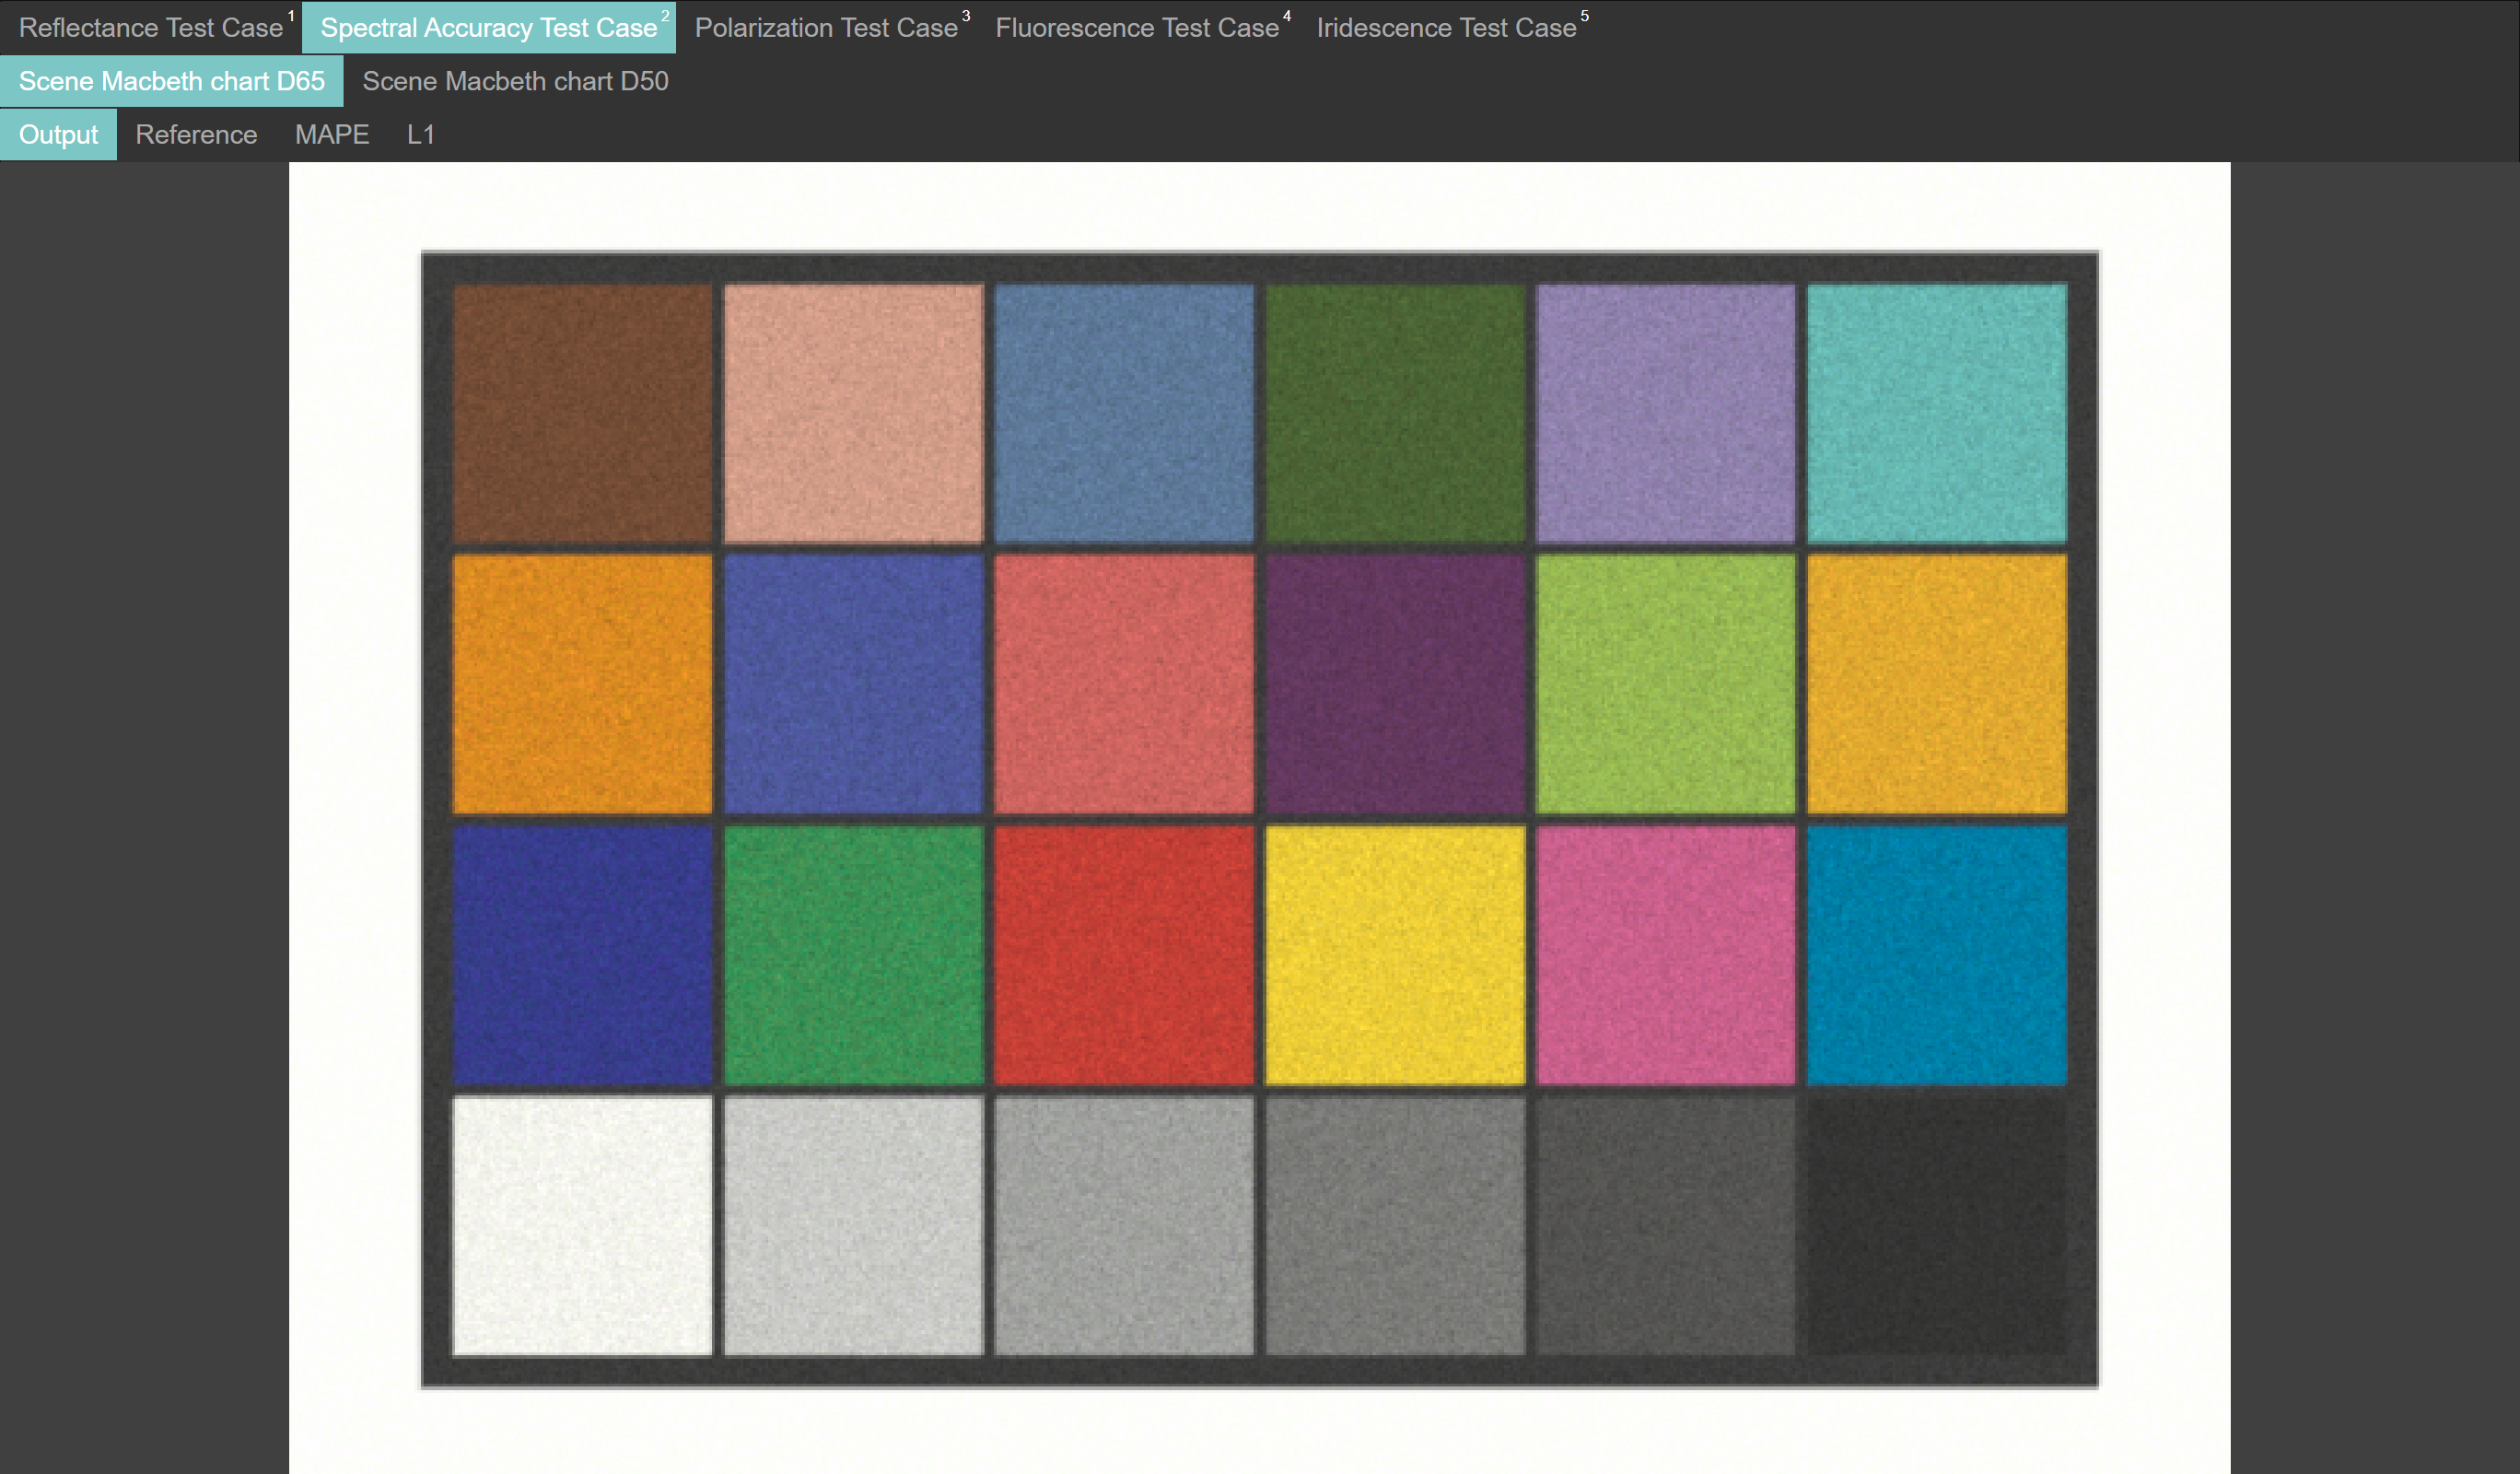
\includegraphics[width=\linewidth]{img/screenshot.png}
	\caption{Results website}
	\label{fig:screenshot}
\end{figure}

\section{Supported Spectral Renderers}

In the current state, the benchmark supports two renderers --- \emph{Mitsuba2} and \emph{ART}. Both are physically-based, research-oriented, they are capable of representing the light in the spectral domain and tracking the polarization states. These features make them suitable candidates for our purposes as we are evaluating the visual correctness of the physically-described appearance phenomena, including spectral accuracy and polarization. The two following sections contain an overview of these renderers.

\subsection{Mitsuba2}

Mitsuba2 has been released only recently (paper was published in November 2019) as a successor to a well-known, research oriented renderer Mitsuba 0.6. Rather than an upgrade, Mitsuba2 is a complete overhaul of its predecessor, incorporating the latest trends in programming. It is very well documented by citet{mitsubaWeb} and \citet{nimier2019mitsuba} and can be downloaded/cloned from \url{https://github.com/mitsuba-renderer/mitsuba2}.

It is written in C++17 and designed to be modular --- it contains a large number of various plugins where each adds a new functionality to the Mitsuba2 rendering process, such as:

\begin{description}
	\item[Materials] BSDFs for rough/smooth dielectrics, conductors, plastic, etc.
	\item[Light sources] Uniform, spot, point, area, environment
	\item[Shapes] Imported obj, ply but also built-in such as sphere
	\item[Integrators] Direct illumination, path tracer, stokes integrator, etc.
\end{description}

and many more.

Mitsuba2 is capable of running in several modes --- from RGB CPU rendering to differentiable GPU spectral rendering that tracks polarization. These options are shown in \autoref{fig:mitsuba_variations}. The important part is that the renderer is retargatable which means that the user may specify the rendering mode without recompiling the project and Mitsuba2 uses the appropriate internal representation of its data. For example, for RGB rendering, the color is obviously represented by an array of 3 floats. For spectral rendering, the array contains 4 floats which represent the spectral wavelengths and a stochastic approach is used to sample these wavelengths. This is possible thanks to the template metaprogramming that C++ offers.

\begin{figure}
	\centering
	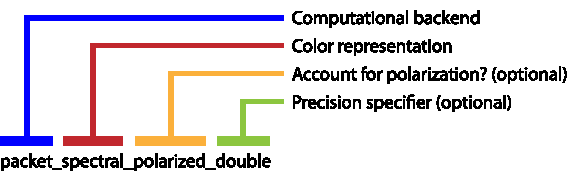
\includegraphics[width=0.8\linewidth]{img/mitsuba_variants.pdf}
	\caption{Different variants of Mitsuba2}
	\label{fig:mitsuba_variations}
\end{figure}

Mitsuba2 also provides an extensive API for Python so that almost all functions may be used from within a code. 

Anyone can contribute to the project via pull request as it is open source.

\subsection{ART}

Advanced Rendering Toolking, or shortly ART, is physically-based, research oriented rendering framework that has been developed by the Computer Graphics Group on Charles University in Prague, Faculty of Mathematics and Physics. In the past, there have been important contributions by people at the Institute of Computer Graphics in Vienna. However, as ART is currently at version 2.0.3, most of their work has not been ported from versions 0.x/1.x. ART can be download/cloned from \url{git://cgg.mff.cuni.cz/ART.git} and this section is largely based on its documentation~\cite{artDoc}.

ART is written in Objective-C and therefore compilable on the majority of the modern operating systems. The scenes are written in a custom language that supports procedural modeling of the scene objects, such as loops and conditions. Also, the immediate results of the rendering process are custom spectral images which contain a lot more information about the wavelengths and the polarization states than standard EXRs. These, however, are not displayable and need to be tonemapped (included in the project) afterwards.

On top of the standard features that most conventional renderers offer, such BSDFs, light sources, camera, path tracing, etc., ART implements several rare, or even unique ones, such as:

\begin{description}
	\item[Spectral rendering] Uses Hero wavelengths spectral sampling
	\item[Fluorescence] Supports fluorescent materials, volumes and even illuminants
	\item[Polarization] Capable of tracking the full polarization state
\end{description}

The whole project includes multiple tools such as polarization visualizer or tonemapper which offers several options for adjusting and converting the spectral images.

As ART is an open source project under GNU v3.0 license therefore anyone can download and use it.

\section{Scenes}
\label{sec:scenes}

This section documents all the test case scenarios and the test scenes that we use in our evaluation process. We look into the specific objects in the scenes, their meaning and we provide justifications for our decisions. Furthermore, each scene follows the same basic principle --- the geometry is supposed to be as simple as possible. The reference images might not be conventionally eye-pleasing because we are aiming for the exact aspects of the features that should confirm the correctness of their computations. Also, the numbers of samples are generally low, as more samples simply make the picture prettier but do not change (after certain threshold) the final color which is what we ultimately want to achieve.

\subsection{GGX Reflectance}

While we mostly focus on the appearance phenomena caused by the spectral rendering, we include the reflectance of rough surfaces to our benchmark, purely because it is still a largely discussed topic. Specifically, we look into the implementations of the GGX microfacet distribution as in most cases, it can be considered the state of the art for rough surfaces. The whole evaluation is based on \citet{walter2007microfacet}.

This test case scenario consists of five scenes:

The first four are done accordingly to the measured data shown in \citet{walter2007microfacet}. Appropriately, we created a scene that contains a single rough copper square under an area light illumination. Depending on the rotation of the plane, we can clearly see the various reflectance distributions, from the visibly illuminated tails at the bottom of the plane to the more sparsely distributed direct illumination at the top. We provide four different rotations --- by 50, 60, 70 and 80 degrees rotated aroud the x-axis. We believe that such granularity is necessary to be completely sure that none of the viewing angles break the implementations. The copper material provides a visible contrast to the dark background as it is more colorful than other metals such as aluminum or silver. This makes the differences clearly visible even to the naked eye. The roughness is set to 0.2 which can be expressed as considerably rough --- less roughness is meaningless as the differences may not be that visible and more roughness could create unrealistically rough surface that could be hard to differentiate from a diffuse. The scenes are separated as we wanted to make sure that only one light illuminates one plane at a time to properly visualize the reflectance distribution. All four scenes are shown in \autoref{fig:ggx_copper}

\begin{figure}[h]
	\begin{tabular}{cc}
		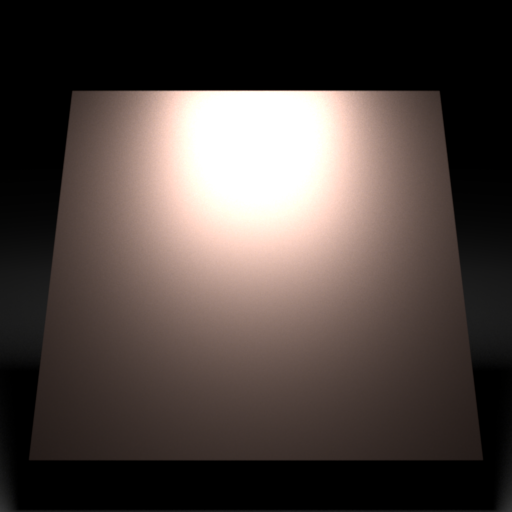
\includegraphics[width=.45\linewidth]{img/ggx_copper_50.png}
		&
		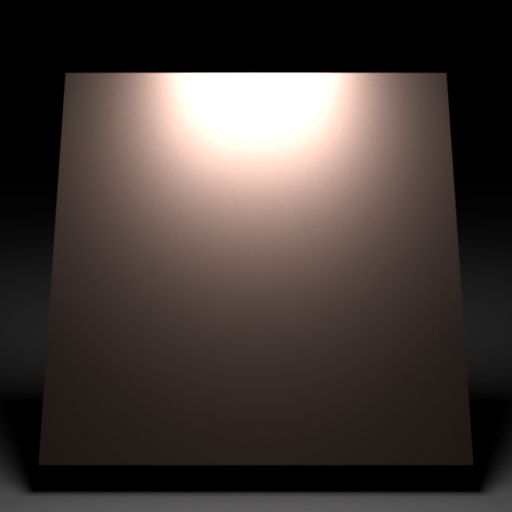
\includegraphics[width=.45\linewidth]{img/ggx_copper_60.png} \\ 
		\includegraphics[width=.45\linewidth]{img/ggx_copper_70.png}
		&
		\includegraphics[width=.45\linewidth]{img/ggx_copper_80.png}
	\end{tabular}
	\caption{Four test scenes consisting of a copper plane with GGX distribution}
	\label{fig:ggx_copper}
\end{figure}

While the previous four scenes tested rough conducting surfaces, the fifth scene demonstrates a rough dielectric --- it consists of a single equally rough dielectric sphere under an area light illumination. We decided to go for a volumetric object instead of the plane for the dielectrics because a dielectric is at least partially transparent and the colors of a plane would predominantly merge with the background. A sphere, however, has its own volume, forming a thick layer in front of the background. Furthermore, testing the very same cases for the dielectrics does not make much sense as we are not really testing the material but the microfacet distribution. A sphere also provides various illumination angles where we can potentially spot the inconsistencies between them. This scene converges pretty slowly for such simple geometry. It is due to the fact that the original GGX needed a quite larger number of samples (256 in our case) to render a plausible result. An improvement has been introduced~\cite{heitz2018sampling} that does not change the distribution but greatly decreases variance. As the article~\cite{walter2007microfacet} mostly compares their GGX approach to the Beckmann distribution, we demonstrate our scene rendered for both distributions in \autoref{fig:ggx_glass}

\begin{figure}[h]
	\begin{tabular}{cc}
		\includegraphics[width=.45\linewidth]{img/ggx_glass.png}
		&
		\includegraphics[width=.45\linewidth]{img/beckmann_glass.png}
	\end{tabular}
	\caption{The test scene consisting of a dielectric sphere with GGX distribution (left) compared to its Beckmann equivalent (right)}
	\label{fig:ggx_glass}
\end{figure}

\subsection{Spectral accuracy}

As the direct representation of the spectral colors is not possible on our screens, we need to make sure that the final image contains colors that actually correspond to the measured data. Distinct renderers may internally represent their color values in a very different manner which might effect the ultimate color that we see.

For these purposes, we use a well-defined set of colors introduced by \citet{mccamy1976color} called \emph{Macbeth chart} or simply \emph{Macbeth colors}. Its basic variant consists of 24 color patches divided in a 4x6 grid, each representing a color that can be normally found in nature --- human skin, flowers, greyscale range, etc. It is primarly used for color calibration therefore it is designed to be stable and invariant under different lighting conditions.

We introduce two scenes that evaluate the correctness of the spectral colors --- both contain a Macbeth chart illuminated by two different standard CIE illuminants, D50 and D65~\cite{cieIlluminants}. As both illuminants and Macbeth colors have exact definitions, they are easily integrated into any renderer that supports spectral color representation. Another advantage is that we know their corresponding RGB values so the results can be easily checked against them.

Note that we assume that the white point of the renderer is indeed D65 (whitepoint of sRGB) for both scenes. Thus, the scene illuminated by the D50 illuminant should have an orange-ish overlay and the scene illuminated by the D65 illuminant should have completely white background.

Both scenes are shown in \autoref{fig:macbeth}. Once the renderer passes this test, we can assume that the representation of the spectral colors is indeed correct. Even though this may seem trivial, testing multiple different materials, colors or even illuminants is simply a variation of our tests with the only difference that we need to evaluate the correctness manually as we do not have the color definitions beforehand.

\begin{figure}[h]
	\begin{tabular}{cc}
		\includegraphics[width=.45\linewidth]{img/macbeth_chart_D50.png}
		&
		\includegraphics[width=.45\linewidth]{img/macbeth_chart_D65.png}
	\end{tabular}
	\caption{The test scenes containing a Macbeth chart under CIE D50 illuminant (left) and under CIE D65 illuminant (right)}
	\label{fig:macbeth}
\end{figure}

\subsection{Polarization}

The polarization cannot be described by a BSDF as GGX or iridescence. It requires a full tracking of the polarization states during the rendering process and ideally a tool that would display these states. Fortunately for us, both ART and Mitsuba2 provide a way to display the results of the Stokes vector as well as polarization filters that are ideal for these kinds of experiments.

The first two scenes use the Brewster's angle (explained in \autoref{sec:polarization}) --- they contain a perfectly reflective dielectric plane (IOR of glass = 1.52) that is illuminated by a single area light under the Brewster's angle. By the definition, the light reflected from the plane is perfectly p-polarized. The difference between the two scenes is in the linear polarizer situated in front of the camera --- in case the transmission axis is horizontally oriented (parallel to the reflected light), the reflection of the light source is clearly visible without any attenuation. However, if the transmission axis is vertically oriented (perpendicurar to the reflected light), there is no reflection of the light source on the plane as the polarizer won't simply let it through. Both scenes are shown in \autoref{fig:polar_planes}.

\begin{figure}[h]
	\begin{tabular}{cc}
		\includegraphics[width=.45\linewidth]{img/polarizing_plane_90.png}
		&
		\includegraphics[width=.45\linewidth]{img/polarizing_plane_0.png}
	\end{tabular}
	\caption{The test scenes with a visible polarized (left) and without a visible polarized light (right)}
	\label{fig:polar_planes}
\end{figure}

The third scene is a lot more specific as it heavily depends on the renderer to be capable of representing the polarization via Stokes vector and visualizing them. This scene contains two smaller dielectric spheres which are in front of a larger smooth conducting sphere illuminated by a constant daylight. The two dielectric spheres create a lot of light polarization which can then be seen on their reflections on the conducting sphere behind them. Note that to ensure the physical plausability, the scenes are monochrome, tracking only the 550nm wavelength. In ART, it is possible to extract the single wavelength information image from its custom spectral image format. In Mitsuba2, we used a workaround by specifying only the 550nm values of all colors inside the scene (light and floor) and by running the rendering process in the monochrome mode. Then, both Mitsuba2 and ART output their results as four distinct images, each representing a different element of the Stokes vector (the complication with the compatibility of the outputs and its solution is explained in \autoref{sec:jeri}). All four images are shown in \autoref{fig:polar_spheres}. Pay attention to the fourth image, which demonstrates that a circular polarization also happened during one of the reflections.

\begin{figure}[h]
	\begin{tabular}{cc}
		\includegraphics[width=.45\linewidth]{img/polarizing_spheres.s0.png}
		&
		\includegraphics[width=.45\linewidth]{img/polarizing_spheres.s1.png} \\
		\includegraphics[width=.45\linewidth]{img/polarizing_spheres.s2.png}
		&
		\includegraphics[width=.45\linewidth]{img/polarizing_spheres.s3.png}
	\end{tabular}
	\caption{The four Stokes vector outputs of a test scence containing polarizing spheres}
	\label{fig:polar_spheres}
\end{figure}

\subsection{Fluorescence}

Fluorescence is one of the four phenomena that are possible thanks to the spectral rendering. As it is not seen on a daily basis, its implementation has been purposely avoided in the vast majority of the renderers. However, as the physical realism begins to be a must-have in the commercial world, its presence is becoming a necessity.

We provide four different test scenes that exercice the fluorescent materials and illuminants and their properties accordingly to their natural behavior. In this case, only ART scenes are provided as Mitsuba2 does not support the feature. 

The test scenes are inspired by \citet{mojzik2018handling}. They all consist of a single yellow-based sphere whereas its properties are essentially various combinations of the absorption spectrum, emission spectrum and the surrounding constant illumination.

\begin{description}
	\item[Daylight, 370nm absorbtion, 650nm emission~\ref{fig:fluorescence_d50_red}] The sphere absorbs 370nm wavelengths and re-emits 650nm while it is placed under the CIE D50 horizon light illuminant. As you can see, the sphere displays a yellow to orange color which is a combination of the yellow base and the emitting red color --- 650nm wavelength is perceived as red. The reason that the sphere is not completely red is due to the lower spectral distribution of the D50 illuminant at 370 nanometers.
	\begin{figure}[H]
		\centering
		\includegraphics[width=.6\linewidth]{img/fluorescent_sphere_D50_red.png}
		\caption{}
		\label{fig:fluorescence_d50_red}
	\end{figure}
	\item[450nm illuminant, 450nm absorbtion, 650 emission~\ref{fig:fluorescent_sphere_mono_red}] The sphere absorbs 450nm wavelengths and re-emits 650nm while it is placed under a monochrome light emitting 450nm wavelengths only (perceived as blue). Intuitively, as the absorbing spectrum and the illuminating spectrum collide, the sphere should emit a brightly red color. This is however slightly attenuated by the yellow base and seems pinkish.
	\begin{figure}[H]
		\centering
		\includegraphics[width=.6\linewidth]{img/fluorescent_sphere_mono_red.png}
		\caption{}
		\label{fig:fluorescent_sphere_mono_red}
	\end{figure}
	\item[450nm illuminant, 370nm absorption, 650 emission~\ref{fig:fluorescent_sphere_mono_invisible}] The sphere absorbs 370nm wavelengths and re-emits 650nm while it is placed under a monochrome light emitting 450nm wavelengths only (perceived as blue). In this case, the two spectral domains do not collide at all. Therefore, the sphere appears to be black due to the missing emission and its opaque surface as there is simply no light to absorb and consquetively nothing to emit. Note that a dielectric would be completely transparent but we do not test this case as it does not concern fluorescence directly but rather the material itself.
	\begin{figure}[H]
		\centering
		\includegraphics[width=.6\linewidth]{img/fluorescent_sphere_mono_invisible.png}
		\caption{}
		\label{fig:fluorescent_sphere_mono_invisible}
	\end{figure}
	\item[Fluo illuminant, non fluo sphere~\ref{fig:fluorescent_sphere_fluoD50_nonfluo}] The sphere has a non-fluorescent yellow material and it is placed under a F8 fluorescent light. As the light directly simulates daylight, the sphere appears to be yellow accordingly to its basis but the backgroung is not purely white due to the inconsistencies between the D50 fluorescent simulator and the actual D50 illuminant.
	\begin{figure}[H]
		\centering
		\includegraphics[width=.6\linewidth]{img/fluorescent_sphere_fluoD50_nonfluo.png}
		\caption{}
		\label{fig:fluorescent_sphere_fluoD50_nonfluo}
	\end{figure}
\end{description}

Many more combinations testing different emitting/absorbing spectral domains and illuminants are possible, however, we believe that they would only be variations of the four test case scenarios mentioned above --- normal light with a fluorescent sphere, monochrome light with the a sphere absorbing different wavelengths, monochrome light with a compatible sphere and fluorescent light with a non-fluorescent sphere.

\subsection{Iridescence}

The evaluation of the iridescence showed some complications as neither Mitsuba2 nor ART natively support the iriderescent effects. The only implementation we found was for Mitsuba version 0.6 introduced by \citet{belcour2017practical}.

We've reimplemented the plugin to Mitsuba2 and used the Mitsuba 0.6 implementation as a reference. The results of the tested scenes have been identical so we consider the Mitsuba2 images as the ground truth.

The implementation simulates the iridescence caused by the light interference in a very thin dielectric film on top of a rough conducting base. There are three parameters that can be set for this iridescent BSDF --- the IOR of the exterior, the IOR of the film and the height of the film. Unfortunately, the final colors of the iridescent effects change rapidly with every even slight variation of the parameters of both the conducting base and the dielectric film. Despite that, there are some consistent changes with the gradual increase of the film height and the film IOR which we are exposing in our test scences. 

Each scene consists of four spheres surrounded by a constant daylight to see the colors as brightly as possible. These spheres have a very low roughness coefficient ($\alpha=0.1$) so that the rough surface does not distort the effect.

\begin{description}
	\item[Film height~\ref{fig:irid_height}] As we've explained in \autoref{sec:irid}, the increasing thickness of the film reduces the visibility of the iridescent effect as there is less light interference. All spheres in this scene have identical base and film IOR --- $\eta_{base}=1.9, \kappa_{base}=1.5, \eta_{film}=1.33$. The first two spheres with the film height equal to 300nm and 550nm are displaying equally visible iridescent effects. The difference is, of course, in their colors as the light interference is largely varying. The film height of the third sphere is quite high, 1500nm, which clearly diminishes the iridescent effect, dominantly displaying the colors of the base. For the reference, the fourth sphere has no film layer on top of it, displaying only the base.
	\begin{figure}[H]
		\centering
		\includegraphics[width=.9\linewidth]{img/iridescent_spheres_height.png}
		\caption{}
		\label{fig:irid_height}
	\end{figure}
	\item[Film IOR~\ref{fig:irid_ior}] Another apparent reaction happens upon the adjustments to the film IOR. With the decreasing IOR of the film, more color fringes can be spotted on the spheres. From the definition of IOR (essentially, how much faster light travels in the vacuum than in the current medium), we can deduce that the faster the light travels through the medium, the interferences happen at higher rate and therefore we can see more colors. The spheres in this scene have identical base and the film height --- $\eta_{base}=1.9, \kappa_{base}=1.5, film\_height=550nm$. The film IORs $\eta_{film}$ are equal to 1.2, 1.5, 1.8 and 2.8, where each consecutive sphere displays one less color fringe that the previous one (from 5 to 2). Please note that the counted amount of the color fringes is not an absolute measure but rather a rough approximation done by a naked eye --- there are a lot more colors in between gradiently transitioning between the fringes and the user may have counted them differently.
	\begin{figure}[H]
		\centering
		\includegraphics[width=.9\linewidth]{img/iridescent_spheres_film.png}
		\caption{}
		\label{fig:irid_ior}
	\end{figure}
	\item[Materials~\ref{fig:irid_mat}] The last scene demonstrates a direct comparison between two well-defined materials (their properties, $\eta_{base}$ and $\kappa_{base}$ provided by Mitsuba) --- copper and mercury --- and their iridescenent equivalents with $\eta_{film}=1.33,film_{height}=550nm$. Both materials emit the same iridescent effect simply put on a  different color base.
	\begin{figure}[H]
		\centering
		\includegraphics[width=.9\linewidth]{img/iridescent_spheres_materials.png}
		\caption{}
		\label{fig:irid_mat}
	\end{figure}
\end{description}

Due to the custom implementation of this plugin for Mitsuba2, we do not evaluate ART is it does not support iridescence at all.

\subsection{Dispersion}

Unfortunately, we do not provide any test scences for dispersion. Mitsuba2 simply does not support the feature which is also explicitly stated in their documentations. ART supports dispersion but we've encountered some issues with the darker colors of the dispersive materials and so we cannot declare the images displaying dispersion generated by ART as the ground truth.

\section{Use cases}

In the following sections, we demonstrate the basic uses cases of our testing suite using a fictional persona called Frodo.

\subsection{Use case Regress test}

Frodo is a mitsuba2 developer who recently changed the sampling strategies of the spectral rendering. However, he is not sure whether he broke some of the functionalities. He sets the benchmark to \texttt{mitsuba2} and provides his latest executable. He runs all test case scenarios and compares the results with the reference images.
 
\subsection{Use case New feature}
\label{sec:frodo}
Frodo is an ART developer who would like to add the GGX microfacet distribution to ART as it is not currently supported in the latest version. He finds the code snippets that are attached to the benchmark suite and integrates them to ART.

Then, he looks up the scenes prepared for Mitsuba2 that test the GGX reflectance and, as these contain only a straightforward geometry, he duplicates them. He saves them in a folder \texttt{/data/cases/reflectance/ART/} and creates \texttt{configuration.json} file in the same folder that only specificies the name of the resulting image, the filename of the test scene and the parameters that are to be passed to the renderer (examples can be seen in different ART scenarios).

Next, he sets the benchmark suite to \texttt{ART} and runs it. The benchmark automatically detects the new configuration for ART. Either from the reference images or from the difference images, he may determine some irregularities that are caused by his incorrect implementation of the masking function. As soon as he corrects it, he sees that the results are coherent.

\subsection{Use case New scenario}

Frodo is a Mitsuba2 developer and he just added support for dispersion. As the dispersion has never been tested before, he simply adds a new folder to the benchmark suite \texttt{/data/cases/dispersion/mitsuba2} and, as in the previous cases, he creates the \texttt{configuration.json} for it.

Now, he must add the keyword \texttt{dispersion} to the string array \texttt{TEXT\_CASES} that can be found in the file \texttt{/src/constants.py}.

From now on, the benchmark contains the dispersion tests as well. If he wants to provide the reference images as well, he may simply store them in the \texttt{/data/references} folder.

In case he also wants to add the new scenario to the visualizer, he needs to extend the file \texttt{/jeri/page/results\_viewer.html}. But, as the HTML page only consists of a simple JSON containing the elements to be displayed, it is fairly easy to do so.

\subsection{Use case Improved feature}

Frodo is an ART developer who reworked the fluorescent materials and would like to see if the new implementation improved them.

The test scenes may be considered as templates, used to create the reference images. Frodo simply adjusts the test scenes in the fluorescence test case scenario to his needs. If he finds out that the results indeed improved, he may replace the existing reference images for the better, adjusted ones.

\subsection{Use case New renderer}

Frodo has created his own spectral renderer the Ring that supports all the test case scenarios in the benchmark suite and he wants to evaluate the correctness of his implementations.

Therefore, he duplicates the template scenes from other renderers accordingly to his own scene format. He creates a new folder for each test case scenario in the \texttt{/data/cases/}, puts his scenes inside accordingly and creates the \texttt{configuration.json} for each of them.

Then, he adds the support for his renderer to the benchmark --- in the \texttt{/src/constants.py} file, he includes the \texttt{ring} keyword to the string array \texttt{RENDERERS}.

Now, he can set the benchmark to evaluate the new Ring renderer. The benchmark pipeline as well as the visualization is done for it automatically.

\section{Open source contributions}

During our work on the benchmark, we have done several noteworthy contributions to three open source projects. Note that these extensions can be considered as byproducts and definitely not the main aim of this thesis --- therefore, they are not yet in a state that can be used for a pull request as this process requires a significant amount of time.

\subsection{GGX for ART}

The use case described in \autoref{sec:frodo} actually happened to us (not to Frodo). As a part of the work on the benchmark, we've decided to add the GGX distribution to the ART renderer and, coincidentally, it nicely correlated with the mentioned scenario. We had the scenes and the reference images prepared for Mitsuba2, we simply replicated them for ART and implemented the GGX. Then, as mentioned in the use, we iterated the benchmark and the adjustments in the code over and over until the results were satisfactory.

The implementation can be found in the attachments of the thesis in \autoref{sec:ggx_art}.

\subsection{Iridescence for Mitsuba2}

Mitsuba does not have a native support for the iridescence but an external plugin has been developed to simulate the iridescent effects of a thin film dielectric layer on top of a rough conductor base. Unfortunately, it was created for Mitsuba version 0.6 and, as Mitsuba2 is fairly new, there has not been an effort to rework the plugin, thus we took the initiative and re-implemented it.

Along with the publication done by \citet{belcour2017practical}, they released a supplementary plugin for Mitsuba 0.6 to demonstrate their results.

There were some major changes to the spectral sampling strategy and the overall object structure done in Mitsuba2 that had to be adapted in the new, re-implemented version of the plugin.

The correctness of the rework has been confirmed in a similar manner to the normal benchmark workflow. We prepared the test case scenerio scenes for the iridescence, rendered them for both Mitsuba2 and Mitsuba 0.6 and considered the latter version to be the ground truth. The implementation can be found on \url{https://github.com/marcel1hruska/mitsuba2} or in the attachments of this thesis~\ref{sec:mitsuba2_irid}.

\subsection{Multi-channel EXR support for jeri.io}
\label{sec:jeri}

While designing the polarization test scenes, we've encountered a compatibility issue between the Stokes vector output format of Mitsuba2 and ART. While ART stores the Stokes vector values into distinct EXR images, Mitsuba2 creates a single multi-channel EXR where each channel contains the Stokes vector information. As you can imagine, such visualization of the rendering results requires a custom solution --- it consists of two parts. First of all, we've added a support for multi-channel EXR images to the JERI framework as there is currently no way to visualize them. It works as follows:

\begin{enumerate}
	\item If the EXR image contains multiple channels, store them in a structure called\texttt{otherChannels} which maps the channel name with its contents.
	\item The user may specify the channel to display in the viewer data.
	\item If the specified channel is in the map, display the wanted contents.
\end{enumerate}

Secondly, we created a highly custom wrapper over the first addition to resolve the incompatibility between the outputs. By default, we assume that the results are stored in four distinct images (similarly to ART), e.g. the file named \texttt{sphere.s0.exr} means that it is the output of the first element in the Stokes vector (the radiance). We test whether such file really exists --- if not, we assume from the name of the file that the user actually wants the channel \texttt{S0} of the file named \texttt{sphere.exr} so we attempt to find it instead of the former one.

This behavior is transparent to the user. If no version of the file exists, the JERI simply displays nothing.

This addition is only a part of the compiled JavaScript code of the JERI. It can be found in the benchmark's file \texttt{/jeri/exr-worker.js} and \texttt{/jeri/jeri.js} between the lines commented as \texttt{multichannel custom support}.
\chapter{Results}
\label{chap:results}

This chapter overviews the results of the evaluation of ART via direct comparison with Mitsuba2. As we've noted before, the fluorescence is exclusive to ART, iridescence to Mitsuba2 and therefore we are not evaluating these as there is no other renderer to compare them with.

Unfortunately, we do not provide any measures that would asses the accuracy of the techniques in an absolute manner, such as accuracy percentage or correctness threshold. Such metric would require an extensive research in the image validation which is out of scope of this thesis. For anyone interested, the verification of the rendering algorithms is discussed in the article by \citet{ulbricht2006verification}.

\section{Error maps}

The only assessment we provide is via difference images. Even though these do not exactly state whether the computation is correct or not, they might help to expose some inaccuracies.

The difference images shown in the following sections are created by L1 and SSIM error maps, both integrated in the JERI framework and consequently in our benchmark. 

\subsection{L1}

\emph{Least absolute deviations}, also known as L1 loss function, computes the absolute difference between the given data and the predicted function:

\begin{equation}
L1=\sum_{i=1}^{n}\mid y_i - f(x_i) \mid
\end{equation}

Generally, it is largely used in the statistical optimizations to find a function that behaves similarly to the given data, minimizing their differences.

In our case, the error map is actually an image that shows the direct differences between the color values for each pixel. This is considered by us to be the absolute basic as it might expose the color inaccuracies that are barely visible to the naked eye.

\subsection{SSIM}
\emph{Structural similarity index measure} (SSIM) is a lot more advanced method, specifically developed by \citet{wang2004image} to measure the loss of data between a reference image and its processed (usually compressed) equivalent. As it is a perceptual metric comparing two images capturing the same scene, we include it in our benchmark.

However, this technique cannot be considered as an absolute metric of correctness either as we often do not let the images to converge completely because of the performance reasons. It is only useful to look at the artifacts exposed by SSIM or to manually increase the number of samples for each scene. 

\section{GGX}

As the GGX implementation for ART was developed by us, it was necessary that we evaluate its correctness. In this section, we discuss the copper plane scene (rotated by 60 degrees) and the glass sphere scene, their implementations in Mitsuba2 and ART and their difference images. All of these images are displayed in \autoref{fig:compare_ggx_copper} and \autoref{fig:compare_ggx_glass}.

\renewcommand\thesubfigure{\arabic{subfigure}}
\begin{figure}[h]
	\centering
	\begin{tabular}{cc}
		\begin{subfigure}
			{0.4\textwidth}\centering\includegraphics[width=\linewidth]{img/ggx_copper_60.png}
			\caption{Mitsuba2 - reference}
		\end{subfigure}
		&
		\begin{subfigure}
			{0.4\textwidth}\centering\includegraphics[width=\linewidth]{img/ggx_copper_60_ART.png}
			\caption{ART - our implementation}
		\end{subfigure} \\
		\begin{subfigure}
			{0.4\textwidth}\centering\includegraphics[width=\linewidth]{img/ggx_copper_60_SSIM.png}
			\caption{SSIM}
		\end{subfigure} 
		&
		\begin{subfigure}
			{0.4\textwidth}\centering\includegraphics[width=\linewidth]{img/ggx_copper_60_L1.png}
			\caption{L1}
		\end{subfigure}
	\end{tabular}
	\caption{Comparisons between the reference image and the ART implementation of the GGX copper plane (rotated by 60 degrees) scene}
	\label{fig:compare_ggx_copper}
\end{figure}

\renewcommand\thesubfigure{\arabic{subfigure}}
\begin{figure}[h]
	\centering
	\begin{tabular}{cc}
		\begin{subfigure}
			{0.4\textwidth}\centering\includegraphics[width=\linewidth]{img/ggx_glass.png}
			\caption{Mitsuba2 - reference}
		\end{subfigure}
		&
		\begin{subfigure}
			{0.4\textwidth}\centering\includegraphics[width=\linewidth]{img/ggx_glass_ART.png}
			\caption{ART - our implementation}
		\end{subfigure} \\
		\begin{subfigure}
			{0.4\textwidth}\centering\includegraphics[width=\linewidth]{img/ggx_glass_SSIM.png}
			\caption{SSIM}
		\end{subfigure} 
		&
		\begin{subfigure}
			{0.4\textwidth}\centering\includegraphics[width=\linewidth]{img/ggx_glass_L1.png}
			\caption{L1}
		\end{subfigure}
	\end{tabular}
	\caption{Comparisons between the reference image and the ART implementation of the GGX glass scene}
	\label{fig:compare_ggx_glass}
\end{figure}

We should note that Mitsuba2 actually implements the improved variant of GGX developed by \citet{heitz2018sampling} which significantly reduces variance. We implemented the original, basic variant~\cite{walter2007microfacet} which logically creates lots of noise for the same amount of samples. Consequently, this diminishes the usability of the SSIM method as the result simply could not converge to the correct state. This is true especially for the glass sphere as there are lot more reflections under various angles than on a simple plane.

However, the L1 function nicely shows that our implementation should be correct. In case of the plane, we see only few dots, signaling that some samples might have brighter colors. In case of the sphere, we can see a larger groups of the dots at the bottom, which is probably caused by the general rough surface model and not the microfacet distribution, as the colors match.

\section{Spectral Accuracy}

The spectral accuracy is significantly harder to quantify and measure as there are lots of mechanisms inside a rendering system that might influence the final colors. Both testing scenes for the spectral accuracy are compared in \autoref{fig:compare_macbeth_d65} and \autoref{fig:compare_macbeth_d50}.

\renewcommand\thesubfigure{\arabic{subfigure}}
\begin{figure}[h]
	\centering
	\begin{tabular}{cc}
		\begin{subfigure}
			{0.4\textwidth}\centering\includegraphics[width=\linewidth]{img/macbeth_chart_D65.png}
			\caption{Mitsuba2 - reference}
		\end{subfigure}
		&
		\begin{subfigure}
			{0.4\textwidth}\centering\includegraphics[width=\linewidth]{img/macbeth_chart_D65_ART.png}
			\caption{ART}
		\end{subfigure} \\
		\begin{subfigure}
			{0.4\textwidth}\centering\includegraphics[width=\linewidth]{img/macbeth_chart_D65_SSIM.png}
			\caption{SSIM}
		\end{subfigure} 
		&
		\begin{subfigure}
			{0.4\textwidth}\centering\includegraphics[width=\linewidth]{img/macbeth_chart_D65_L1.png}
			\caption{L1}
		\end{subfigure}
	\end{tabular}
	\caption{Comparisons between the reference image and the ART implementation of the Macbeth chart D65 scene}
	\label{fig:compare_macbeth_d65}
\end{figure}

\renewcommand\thesubfigure{\arabic{subfigure}}
\begin{figure}[h]
	\centering
	\begin{tabular}{cc}
		\begin{subfigure}
			{0.4\textwidth}\centering\includegraphics[width=\linewidth]{img/macbeth_chart_D50.png}
			\caption{Mitsuba2 - reference}
		\end{subfigure}
		&
		\begin{subfigure}
			{0.4\textwidth}\centering\includegraphics[width=\linewidth]{img/macbeth_chart_D50_ART.png}
			\caption{ART}
		\end{subfigure} \\
		\begin{subfigure}
			{0.4\textwidth}\centering\includegraphics[width=\linewidth]{img/macbeth_chart_D50_SSIM.png}
			\caption{SSIM}
		\end{subfigure} 
		&
		\begin{subfigure}
			{0.4\textwidth}\centering\includegraphics[width=\linewidth]{img/macbeth_chart_D50_L1.png}
			\caption{L1}
		\end{subfigure}
	\end{tabular}
	\caption{Comparisons between the reference image and the ART implementation of the Macbeth chart D50 scene}
	\label{fig:compare_macbeth_d50}
\end{figure}

On the first sight, the two images are extremely similar --- the spectral definitions for the Macbeth colors and the illuminants are the very same for both renderers which is backed by the L1 comparisons. But as we look on the SSIM, there are slight variations in different color patches. The Macbeth blue and black are accurate but for some reason the others, especially yellow and yellow-green are slightly more saturated in the reference images. This might indicate a potential flow in the stochastic approach of spectral sampling in Mitsuba2 but as the differences are barely there, we do not consider the results to be incorrect. Note that the two SSIM images are almost identical which shows that the relative comparison under the same lighting conditions matches.  

\section{Polarization}

Unfortunately for us, it is quite complicated to directly compare the outputs of the Stokes vectors as the final format heavily depends on the renderer. To make the matters as simple as possible, the scene is monochrome and tracks a single-wavelength light only. We compare the visualization of the horizontal/vertical polarization stored in the Stokes vector in \autoref{fig:compare_polar_s1}. 

The second discussed scene is shown in \autoref{fig:compare_polar_angle} and demonstrates the polarizing plane scene with a visible reflection.

\renewcommand\thesubfigure{\arabic{subfigure}}
\begin{figure}[h]
	\centering
	\begin{tabular}{cc}
		\begin{subfigure}
			{0.4\textwidth}\centering\includegraphics[width=\linewidth]{img/polarizing_spheres.s1.png}
			\caption{Mitsuba2 - reference}
		\end{subfigure}
		&
		\begin{subfigure}
			{0.4\textwidth}\centering\includegraphics[width=\linewidth]{img/polarizing_spheres.s1_ART.png}
			\caption{ART}
		\end{subfigure} \\
		\begin{subfigure}
			{0.4\textwidth}\centering\includegraphics[width=\linewidth]{img/polarizing_spheres.s1_SSIM.png}
			\caption{SSIM}
		\end{subfigure} 
		&
		\begin{subfigure}
			{0.4\textwidth}\centering\includegraphics[width=\linewidth]{img/polarizing_spheres.s1_L1.png}
			\caption{L1}
		\end{subfigure}
	\end{tabular}
	\caption{Comparisons between the reference image and the ART implementation of the second Stokes vector element of the polarizing spheres scene}
	\label{fig:compare_polar_s1}
\end{figure}

\renewcommand\thesubfigure{\arabic{subfigure}}
\begin{figure}[h]
	\centering
	\begin{tabular}{cc}
		\begin{subfigure}
			{0.4\textwidth}\centering\includegraphics[width=\linewidth]{img/polarizing_plane_90.png}
			\caption{Mitsuba2 - reference}
		\end{subfigure}
		&
		\begin{subfigure}
			{0.4\textwidth}\centering\includegraphics[width=\linewidth]{img/polarizing_plane_90_ART.png}
			\caption{ART}
		\end{subfigure} \\
		\begin{subfigure}
			{0.4\textwidth}\centering\includegraphics[width=\linewidth]{img/polarizing_plane_90_SSIM.png}
			\caption{SSIM}
		\end{subfigure} 
		&
		\begin{subfigure}
			{0.4\textwidth}\centering\includegraphics[width=\linewidth]{img/polarizing_plane_90_L1.png}
			\caption{L1}
		\end{subfigure}
	\end{tabular}
	\caption{Comparisons between the reference image and the ART implementation of the polarizing plane (filter rotated by 90 degrees) scene}
	\label{fig:compare_polar_angle}
\end{figure}

The polarizing plane scene might seem to be more attenuated in case of ART, especially under the plane. However, this does not concern us as the purpose of the scene is to expose the behavior of the unpolarized light upon the interaction with a surface under a Brewster's angle rather than the material's transmission properties. Neither of the difference images show obvious inconsistencies but both are suggesting that the reflection of the light on the plane is at least partially off.

After the simplifications done to the polarizing spheres scene, we can see that the results are almost identical. But, there is  a visible difference in the vertical polarization on the spheres (properly exposed by SSIM) and we could conclude that Mitsuba2 does not track completely unpolarized light properly. However, bear in mind that the images we compare are not airect results of the rendering process but rather a byproduct of a specific structure inside it so it might simply be a color output inconsistency rather than a polarization tracking flaw.

\chapter*{Conclusion}
\addcontentsline{toc}{chapter}{Conclusion}


%%% Bibliography
%%% Bibliography (literature used as a source)
%%%
%%% We employ bibTeX to construct the bibliography. It processes
%%% citations in the text (e.g., the \cite{...} macro) and looks up
%%% relevant entries in the bibliography.bib file.
%%%
%%% The \bibliographystyle command selects, which style will be used
%%% for references from the text. The argument in curly brackets is
%%% the name of the corresponding style file (*.bst). Both styles
%%% mentioned in this template are included in LaTeX distributions.

\bibliographystyle{plainnat}    %% Author (year)
% \bibliographystyle{unsrt}     %% [number]

\renewcommand{\bibname}{Bibliography}

%%% Generate the bibliography. Beware that if you cited no works,
%%% the empty list will be omitted completely.

\bibliography{bibliography}

%%% If case you prefer to write the bibliography manually (without bibTeX),
%%% you can use the following. Please follow the ISO 690 standard and
%%% citation conventions of your field of research.

% \begin{thebibliography}{99}
%
% \bibitem{lamport94}
%   {\sc Lamport,} Leslie.
%   \emph{\LaTeX: A Document Preparation System}.
%   2nd edition.
%   Massachusetts: Addison Wesley, 1994.
%   ISBN 0-201-52983-1.
%
% \end{thebibliography}


%%% Figures used in the thesis (consider if this is needed)
%%%\listoffigures

%%% Tables used in the thesis (consider if this is needed)
%%% In mathematical theses, it could be better to move the list of tables to the beginning of the thesis.
%%%\listoftables

%%% Abbreviations used in the thesis, if any, including their explanation
%%% In mathematical theses, it could be better to move the list of abbreviations to the beginning of the thesis.
%%%\chapwithtoc{List of Abbreviations}

%%% Attachments to the master thesis, if any. Each attachment must be
%%% referred to at least once from the text of the thesis. Attachments
%%% are numbered.
%%%
%%% The printed version should preferably contain attachments, which can be
%%% read (additional tables and charts, supplementary text, examples of
%%% program output, etc.). The electronic version is more suited for attachments
%%% which will likely be used in an electronic form rather than read (program
%%% source code, data files, interactive charts, etc.). Electronic attachments
%%% should be uploaded to SIS and optionally also included in the thesis on a~CD/DVD.
%%% Allowed file formats are specified in provision of the rector no. 72/2017.
\appendix
\chapter{User Guide}

The user may clone/download the benchmark from the github repository \url{https://github.com/marcel1hruska/render_benchmark} or he can find it in the attachments of thesis~\ref{sec:benchmark}. As the whole benchmark is written in Python3, there is no need to compile the project. 

Firstly, it is necessary to modify \texttt{settings.json} file in the root directory of the benchmark suite --- the user must specify the path to the renderer executable and the name of the renderer (currently, the only viable options are \texttt{mitsuba2} and \texttt{ART}).

After that, the benchmark can be run with a simple invocation of the \\ \texttt{benchmark.py} python file. Note that the script must be invoked from within the root directory of the benchmark suite! For example, you can do so by issuing the following commands inside Ubuntu bash:

\begin{lstlisting}
cd /render_benchmark
python3 ./benchmark.py
\end{lstlisting}

The benchmark accepts several parameters:
\begin{description}
	\item[-{}-help (-h)] Prints the help message
	\item[-{}-scene (-s) \textless scene\_name\textgreater] Test only the scene called scene\_name
	\item[-{}-case (-c) \textless test\_case\_name\textgreater] Test only the test case called test\_case\_name
	\item[-{}-renderer (-r) [ART/mitsuba2]] Specify the name of the renderer 
	\item[-{}-exec (-e) \textless path\textgreater] Specify the path to the renderer executable
	\item[-{}-log (-l)] Write all outputs to the log file (in the outputs folder) instead of the console
	\item[-{}-visualize (-v)] Visualize the outputs immediately after the benchmark ends
\end{description}

For the user's convenience, all of these options may be specified in the \\ \texttt{settings.json} file but the ones issued in the CLI take higher priority and override them.

As soon as the benchmark ends, the user may find the rendered EXR images in a folder named \texttt{outputs-yyymmdd-hhmmss} where the \texttt{yyymmdd-hhmmss} is substituted for the date and then time when the command was issued.

Then, the user may invoke a second script, \texttt{visualize.py}, that opens a website with the results of the last benchmark run along with the reference images and their difference images. This script must also be run from within the root directory of the benchmark suite. It accepts only two parameters:

\begin{description}
	\item[-{}-help (-h)] Prints the help message
	\item[-{}-outputs (-o) \textless output\_folder\_name\textgreater] Specify the name of the\\ \texttt{outputs-yyymmdd-hhmmss} folder that is to be visualized. If omitted, the latest folder is picked.
\end{description}


\chapter{Attachments}

All attachments are listed below and can be found in the \texttt{attachments} folder. 

\section{Benchmark}
\label{sec:benchmark}

Contains the whole testing suite, can also be downloaded from \url{https://github.com/marcel1hruska/render_benchmark}. If the user downloaded the thesis from github, he needs to do so recursively as the \texttt{render\_benchmark} is a submodule.

\section{Iridescence for Mitsuba2}
\label{sec:mitsuba2_irid}

Contains the iridescence implementation for Mitsuba2. The folder can be simply copied over the Mitsuba2 code version 2.1.0. Note that only the \texttt{iridescence.h} and \texttt{iridescence.cpp} files contain our code --- the rest of the code mostly belongs to Mitsuba2 and only small parts that activate the iridescent effects were created by us. 

To make matters more simple, we created a forked repository on \url{https://github.com/marcel1hruska/mitsuba2}. The user needs to checkout the \\ \texttt{iridescence} branch and compile it accordingly to the Mitsuba2 documentation~\cite{mitsubaWeb}.

\section{GGX for ART}
\label{sec:ggx_art}

Contains the GGX implementation for ART. The folder can be simply copied over the ART code version 2.0.3. Note that the files also include the implementation of the Blinn microfacet distribution which belongs to ART and is not a part of this thesis. 

Unfortunately, we do not have a fork of the repository as the origin is not on github.

\openright
\end{document}
